% ******************************* PhD Thesis Template **************************
% Please have a look at the README.md file for info on how to use the template

\documentclass[a4paper, 12pt, custombib, customfont, print]{Classes/PhDThesisPSnPDF}

% ******************************************************************************
% ******************************* Class Options ********************************
% *********************** See README for more details **************************
% ******************************************************************************

% `a4paper'(The University of Cambridge PhD thesis guidelines recommends a page
% size a4 - default option) or `a5paper': A5 Paper size is also allowed as per
% the Cambridge University Engineering Deparment guidelines for PhD thesis
%
% `11pt' or `12pt'(default): Font Size 10pt is NOT recommended by the University
% guidelines
%
% `oneside' or `twoside'(default): Printing double side (twoside) or single
% side.
%
% `print': Use `print' for print version with appropriate margins and page
% layout. Leaving the options field blank will activate Online version.
%
% `index': For index at the end of the thesis
%
% `draftclassic': For draft mode without loading any images (same as draft in book)
%
% `draft': Special draft mode with line numbers, images, and water mark with
% timestamp and custom text. Position of the text can also be modified.
%
% `abstract': To generate only the title page and abstract page with
% dissertation title and name, to submit to the Student Registry
%
% `chapter`: This option enables only the specified chapter and it's references
%  Useful for review and corrections.
%
% ************************* Custom Page Margins ********************************
%
% `custommargin`: Use `custommargin' in options to activate custom page margins,
% which can be defined in the preamble.tex. Custom margin will override
% print/online margin setup.
%
% *********************** Choosing the Fonts in Class Options ******************
%
% `times' : Times font with math support. (The Cambridge University guidelines
% recommend using times)
%
% `fourier': Utopia Font with Fourier Math font (Font has to be installed)
%            It's a free font.
%
% `customfont': Use `customfont' option in the document class and load the
% package in the preamble.tex
%
% default or leave empty: `Latin Modern' font will be loaded.
%
% ********************** Choosing the Bibliography style ***********************
%
% `authoryear': For author-year citation eg., Krishna (2013)
%
% `numbered': (Default Option) For numbered and sorted citation e.g., [1,5,2]
%
% `custombib': Define your own bibliography style in the `preamble.tex' file.
%              `\RequirePackage[square, sort, numbers, authoryear]{natbib}'.
%              This can be also used to load biblatex instead of natbib
%              (See Preamble)
%
% **************************** Choosing the Page Style *************************
%
% `default (leave empty)': For Page Numbers in Header (Left Even, Right Odd) and
% Chapter Name in Header (Right Even) and Section Name (Left Odd). Blank Footer.
%
% `PageStyleI': Chapter Name next & Page Number on Even Side (Left Even).
% Section Name & Page Number in Header on Odd Side (Right Odd). Footer is empty.
%
% `PageStyleII': Chapter Name on Even Side (Left Even) in Header. Section Number
% and Section Name in Header on Odd Side (Right Odd). Page numbering in footer

% Uncomment to change page style
%\pagestyle{PageStyleII}

% ********************************** Preamble **********************************
% Preamble: Contains packages and user-defined commands and settings
% ******************************************************************************
% ****************************** Custom Margin *********************************

% Add `custommargin' in the document class options to use this section
% Set {innerside margin / outerside margin / topmargin / bottom margin}  and
% other page dimensions
\ifsetCustomMargin
  \RequirePackage[left=37mm,right=30mm,top=35mm,bottom=30mm]{geometry}
  \setFancyHdr % To apply fancy header after geometry package is loaded
\fi

% Add spaces between paragraphs
%\setlength{\parskip}{0.5em}
% Ragged bottom avoids extra whitespaces between paragraphs
\raggedbottom
% To remove the excess top spacing for enumeration, list and description
%\usepackage{enumitem}
%\setlist[enumerate,itemize,description]{topsep=0em}

% *****************************************************************************
% ******************* Fonts (like different typewriter fonts etc.)*************

% Add `customfont' in the document class option to use this section

\ifsetCustomFont
  % Set your custom font here and use `customfont' in options. Leave empty to
  % load computer modern font (default LaTeX font).
  %\RequirePackage{helvet}

\usepackage{polyglossia}
\usepackage[autostyle=true]{csquotes}

\setmainlanguage[variant=mono]{greek}
\setotherlanguage{english}

\usepackage{amsmath}
\usepackage[]{unicode-math}
\setmainfont{XITS}
[    Extension = .otf,
   UprightFont = *-Regular,
      BoldFont = *-Bold,
    ItalicFont = *-Italic,
BoldItalicFont = *-BoldItalic,
]

\setmathfont{XITSMath-Regular}
[    Extension = .otf,
     BoldFont = XITSMath-Bold,
]

\newfontfamily\greekfont[Script=Greek]{XITS}
\newfontfamily\greekfontsf[Script=Greek]{XITS}
\newfontfamily\greekmathfont{XITSMath-Regular}


  % For use with XeLaTeX
  %  \setmainfont[
  %    Path              = ./libertine/opentype/,
  %    Extension         = .otf,
  %    UprightFont = LinLibertine_R,
  %    BoldFont = LinLibertine_RZ, % Linux Libertine O Regular Semibold
  %    ItalicFont = LinLibertine_RI,
  %    BoldItalicFont = LinLibertine_RZI, % Linux Libertine O Regular Semibold Italic
  %  ]
  %  {libertine}
  %  % load font from system font
  %  \newfontfamily\libertinesystemfont{Linux Libertine O}
\fi

% *****************************************************************************
% **************************** Custom Packages ********************************
% ************************* Algorithms and Pseudocode **************************

%\usepackage{algpseudocode}


% ********************Captions and Hyperreferencing / URL **********************

% Captions: This makes captions of figures use a boldfaced small font.
%\RequirePackage[small,bf]{caption}

\RequirePackage[labelsep=space, tableposition=top, textfont=it]{caption}
\renewcommand{\thefigure}{\thechapter.\arabic{figure}}
\renewcommand{\thetable}{\thechapter.\arabic{table}}
\renewcommand{\figurename}{Figure} %to support older versions of captions.sty

\usepackage{prettyref}
\newrefformat{ch}{Κεφάλαιο~\ref{#1}}
\newrefformat{app}{Παράρτημα~\ref{#1}}
\newrefformat{fig}{Σχήμα~\ref{#1}}
\newrefformat{tab}{Πίνακας~\ref{#1}}
\newrefformat{plt}{Γράφημα~\ref{#1}}
\newrefformat{eq}{σχέση~\ref{#1}}
\newrefformat{code}{Αλγόριθμο~\ref{#1}}

% *************************** Graphics and figures *****************************

%\usepackage{rotating}
%\usepackage{wrapfig}

% Uncomment the following two lines to force Latex to place the figure.
% Use [H] when including graphics. Note 'H' instead of 'h'0
%\usepackage{float}
%\restylefloat{figure}

% Subcaption package is also available in the sty folder you can use that by
% uncommenting the following line
% This is for people stuck with older versions of texlive
%\usepackage{sty/caption/subcaption}
\usepackage{subcaption}

% ********************************** Tables ************************************
\usepackage{booktabs} % For professional looking tables
\usepackage{multirow}
\usepackage{multicol}
\usepackage{longtable}
\usepackage{tabularx}

% ********************************** Plotting within LaTeX **********************
\usepackage{pgfplots}
\pgfplotsset{compat=1.8}
\usepackage{pgfplotstable}
\usepackage{filecontents}

\usepackage{tikz}
\usetikzlibrary{shapes, arrows, shapes.multipart}


% *********************************** SI Units *********************************
\usepackage[detect-all]{siunitx} % use this package module for SI units


% ******************************* Line Spacing *********************************
\usepackage{float}
% Choose linespacing as appropriate. Default is one-half line spacing as per the
% University guidelines

% \doublespacing
% \onehalfspacing
% \singlespacing


% ************************ Formatting / Footnote *******************************

% Don't break enumeration (etc.) across pages in an ugly manner (default 10000)
%\clubpenalty=500
%\widowpenalty=500

%\usepackage[perpage]{footmisc} %Range of footnote options


% *****************************************************************************
% *************************** Bibliography  and References ********************

%\usepackage{cleveref} %Referencing without need to explicitly state fig /table

% Add `custombib' in the document class option to use this section
\ifuseCustomBib
%   \RequirePackage[square, sort, numbers, authoryear]{natbib} % CustomBib

% If you would like to use biblatex for your reference management, as opposed to the default `natbibpackage` pass the option `custombib` in the document class. Comment out the previous line to make sure you don't load the natbib package. Uncomment the following lines and specify the location of references.bib file

\RequirePackage[backend=biber, style=numeric-comp,
				citestyle=numeric, sorting=nty,
				isbn=false, doi=true,
				url = false, natbib=false,
				defernumbers=true]{biblatex}
\addbibresource{References/references.bib} %Location of references.bib only for biblatex, Do not omit the .bib extension from the filename.

\fi

% changes the default name `Bibliography` -> `References'
%\renewcommand{\bibname}{References}


% ******************************************************************************
% ************************* User Defined Commands ******************************
% ******************************************************************************

% *********** To change the name of Table of Contents / LOF and LOT ************


%\renewcommand{\contentsname}{My List of Contents}
%\renewcommand{\listfigurename}{My List of Figures}
%\renewcommand{\listtablename}{Λίστα πινάκων}


% ********************** TOC depth and numbering depth *************************

\setcounter{secnumdepth}{2}
\setcounter{tocdepth}{2}


% ******************************* nomenclature *********************************

% Increase spacing between notation and text
\setlength{\nomlabelwidth}{1.5cm}

% To decrease the spacing between two consecutive notations
%\setlength{\nomitemsep}{-\parsep}

% To change the name of the Nomenclature section, uncomment the following line
\renewcommand{\nomname}{Αποδόσεις όρων}


% ********************************* Appendix ***********************************

% The default value of both \appendixtocname and \appendixpagename is `Appendices'. These names can all be changed via:

%\renewcommand{\appendixtocname}{List of appendices}
%\renewcommand{\appendixname}{Appndx}

% *********************** Configure Draft Mode **********************************

% Uncomment to disable figures in `draft'
%\setkeys{Gin}{draft=true}  % set draft to false to enable figures in `draft'

% These options are active only during the draft mode
% Default text is "Draft"
%\SetDraftText{DRAFT}

% Default Watermark location is top. Location (top/bottom)
%\SetDraftWMPosition{bottom}

% Draft Version - default is v1.0
%\SetDraftVersion{v1.1}

% Draft Text grayscale value (should be between 0-black and 1-white)
% Default value is 0.75
%\SetDraftGrayScale{0.8}


% ******************************** Todo Notes **********************************
%% Uncomment the following lines to have todonotes.

%\ifsetDraft
%	\usepackage[colorinlistoftodos]{todonotes}
%	\newcommand{\mynote}[1]{\todo[author=kks32,size=\small,inline,color=green!40]{#1}}
%\else
%	\newcommand{\mynote}[1]{}
%	\newcommand{\listoftodos}{}
%\fi

% Example todo: \mynote{Hey! I have a note}

% *****************************************************************************
% ******************* Better enumeration my MB*************
\usepackage{enumitem}


% ******************************** Typesetting Matlab Code **********************

\usepackage{bigfoot, textcomp, listings, xspace, fancyvrb}
\usepackage[numbered, framed, final]{matlab-prettifier}

\lstset{
  style              = Matlab-editor,
  basicstyle         = \mlttfamily,
  mlshowsectionrules = true,
  texcl=true,
  escapebegin=\begin{english},
  escapeend=\end{english},
  extendedchars =\true,
  aboveskip=20pt,
  belowskip=20pt
}


\usepackage[breakable]{tcolorbox}
\tcbuselibrary{listings}
\usepackage{algorithm2e, setspace, courier}
\tcbset{
  noparskip/.style={before={\par\smallskip\pagebreak[0]\parindent=0pt },
                    after={\par\smallskip}}
}

% redefine \VerbatimInput
\RecustomVerbatimCommand{\VerbatimInput}{VerbatimInput}%
{fontsize=\footnotesize,
 %
 frame=lines,  % top and bottom rule only
 framesep=2em, % separation between frame and text
 rulecolor=\color{Gray},
 %
 label=\fbox{\color{Black}results.txt},
 labelposition=topline
 %
% commandchars=\|\(\), % escape character and argument delimiters for
                      % commands within the verbatim
% commentchar=*        % comment character
}


\renewcommand{\lstlistingname}{Αλγόριθμος}
\renewcommand{\lstlistlistingname}{Λίστα αλγορίθμων}

\newcommand{\matlab}{\textsc{MATLAB}\textsuperscript{\textregistered}\xspace}
\newcommand{\inkscape}{\textit{Inkscape}\textsuperscript{\textcopyright}\xspace}

% ******************************** Macros used **********************************

\newcommand{\volume}{\ooalign{$V$\cr\raisebox{0.15em}{\kern0.08em\textendash}\cr}}

\makeatletter
\renewcommand{\@chapapp}{}% Not necessary...
\newenvironment{chapquote}[2][2em]
  {\setlength{\@tempdima}{#1}%
   \def\chapquote@author{#2}%
   \parshape 1 \@tempdima \dimexpr\textwidth-2\@tempdima\relax%
   \itshape}
  {\par\normalfont\hfill\textendash\ \chapquote@author\hspace*{\@tempdima}\par\bigskip}
\makeatother

\newcommand{\ITU}{İTÜ}
\newcommand{\TikZ}{Ti\textit{k}Z\xspace}

\newcommand{\ra}[1]{\renewcommand{\arraystretch}{#1}}

% ******************************** Miscellany ************************************
\definecolor{SchoolColor}{RGB}{11, 66, 104}
\usepackage{lettrine, adjustbox, threeparttable}
%\usepackage{pdflscape} %adds the attribute /Rotate in a landscape

%\addto\captionsenglish{\renewcommand{\chaptername}{Lecture}}
\makeatletter
\renewcommand{\@chapapp}{Κεφάλαιο}
\makeatother

\usepackage{cancel} % cancel terms out it math equations

\hyphenation{ρευ-στο-μη-χα-νι-κής}
\hyphenation{Ü-ni-ve-rsi-te-si}
\hyphenation{Μη-χα-νο-λό-γων}
\hyphenation{Πα-νε-πι-στή-μιο}
\hyphenation{Ε-κδό-σεις}

% ************************ Thesis Information & Meta-data **********************
% Thesis title and author information, refernce file for biblatex
% ************************ Thesis Information & Meta-data **********************
%% The title of the thesis
\title{Πειραματική μελέτη περιδινούμενης ροής και μετάδοσης θερμότητας σε ομόκεντρους κυλίνδρους με εφαπτομενική
ροή εισόδου}
%\texorpdfstring is used for PDF metadata. Usage:
%\texorpdfstring{LaTeX_Version}{PDF Version (non-latex)} eg.,
%\texorpdfstring{$sigma$}{sigma}

%% Subtitle (Optional)
% \subtitle{Using the CUED template}

%% The full name of the author
\author{Δαρμάνης Μιχαήλ}

%% Department (eg. Department of Engineering, Maths, Physics)
\dept{Τμήμα Μηχανολόγων Μηχανικών}

%% University and Crest
\university{Πανεπιστήμιο Δυτικής Αττικής}
% Crest minimum should be 30mm.
\crest{
\includegraphics[width=0.35\textwidth]{uniwa_crest}}
%% Use this crest, if you are using the college crest
%% Crest long miminum should be 65mm
%\crest{
\includegraphics[width=0.45\textwidth]{uniwa_crest_long}}

%% College shield [optional] 
% Crest minimum should be 30mm.
%\collegeshield{
\includegraphics[width=0.2\textwidth]{CollegeShields/Kings}}


%% Supervisor (optional)
%% for multiple supervisors, append each supervisor with the \newline command
%\supervisor{Καθ. Κωνσταντίνος-Στέφανος Νίκας}
%\supervisor{Prof. A.B. Supervisor\newline
%Prof. C.D. Supervisor}

%% Supervisor Role (optional) - Supervisor (default) or advisor
%\supervisorrole{\textbf{Επιβλέπων: }}
% \supervisorrole{\textbf{Supervisors: }}
%% if no title is desired:
% \supervisorrole{}

%% Supervisor line width: required to align supervisors
%\supervisorlinewidth{0.35\textwidth}

%% Advisor (optional)
%% for multiple advisors, append each advisor with the \newline command
%\advisor{Dr. A. Advisor\newline
%Dr. B. Advisor}
     
%% Advisor Role (optional) - Advisor (default) or leave empty
% \advisorrole{Advisors: }
%% if no title is required
% \advisorrole{}

%% Advisor line width: required to align supervisors
%\advisorlinewidth{0.25\textwidth}


%% You can redefine the submission text:
% Default as per the University guidelines:
% ``This dissertation is submitted for the degree of''
\renewcommand{\submissiontext}{Η παρούσα εργασία υποβάλλεται προς έγκριση τίτλου}

%% Full title of the Degree
\degreetitle{Μηχανολόγου Μηχανικού Τ.Ε.}

%% College affiliation (optional)
\college{Πειραιάς, Αιγάλεω}

%% Submission date
% Default is set as {\monthname[\the\month]\space\the\year}
\degreedate{Φεβρουάριος\space\the\year} 

%% Meta information
\subject{LaTeX} \keywords{{LaTeX} {Bsc Thesis} {Engineering} {University of 
West Attica}}


% ***************************** Abstract Separate ******************************
% To printout only the titlepage and the abstract with the PhD title and the
% author name for submission to the Student Registry, use the `abstract' option in
% the document class.

\ifdefineAbstract
 \pagestyle{empty}
 \includeonly{Declaration/declaration, Abstract/abstract}
\fi

% ***************************** Chapter Mode ***********************************
% The chapter mode allows user to only print particular chapters with references
% Title, Contents, Frontmatter are disabled by default
% Useful option to review a particular chapter or to send it to supervisior.
% To use choose `chapter' option in the document class

\ifdefineChapter
 \includeonly{Chapter3/chapter3}
\fi

% ******************************** Front Matter ********************************
\begin{document}

\frontmatter

\maketitle

{\cleardoublepage
\setsinglecolumn
\thispagestyle{empty}

\null\vfill
\begin{center}
  Η πτυχιακή του Δαρμάνη Μιχαήλ εγκρίθηκε από την επιτροπή: \\

  \vspace{.25in} \vspace{.75in}
  $\:\overline{~~~~ \mbox{\rule{0in}{0.16in} \hspace{3.5in}}}\:$ \\
  \textbf{Κωνσταντίνος-Στέφανος Νίκας} \\
  Καθηγητής ΠΑ.Δ.Α. \\
  (επιβλέπων) \\

  \vspace{.75in}
  $\:\overline{~~~~ \mbox{\rule{0in}{0.16in} \hspace{3.5in}}}\:$ \\
  \textbf{Κωνσταντίνος Μουστρής} \\
  Αναπληρωτής Καθηγητής ΠΑ.Δ.Α. \\

  \vspace{.75in}
  $\:\overline{~~~~ \mbox{\rule{0in}{0.16in} \hspace{3.15in}}}\:$ \\
  \vspace{.3pt} \textbf{Ιωάννης Σιγάλας} \\
  Εργαστηριακό Διδακτικό Προσωπικό ΠΑ.Δ.Α. \\
  \vspace{.75in}
  \vspace{-.25in}
  \vspace{.75in}
  Φεβρουάριος\space\the\year
\end{center}
\vfill\null}
% ******************************* Thesis Declaration ***************************

\begin{declaration}

\noindent Ο κάτωθι υπογεγραμμένος \textbf{Δαρμάνης Μιχαήλ} του \textbf{Παναγιώτη}, με αριθμό μητρώου \textit{36093}, φοιτητής του Πανεπιστημίου Δυτικής Αττικής της Σχολής Μηχανικών, του Τμήματος Μηχανολόγων Μηχανικών, δηλώνω υπεύθυνα ότι: 

\enquote{Είμαι συγγραφέας αυτής της πτυχιακής εργασίας και ότι κάθε βοήθεια την οποία είχα για την προετοιμασία της είναι πλήρως αναγνωρισμένη και αναφέρεται στην εργασία. Επίσης, οι όποιες πηγές από τις οποίες έκανα χρήση δεδομένων, ιδεών ή λέξεων, είτε ακριβώς είτε παραφρασμένες, αναφέρονται στο σύνολό τους, με πλήρη αναφορά στους συγγραφείς, τον εκδοτικό οίκο ή το περιοδικό, συμπεριλαμβανομένων και των πηγών που ενδεχομένως χρησιμοποιήθηκαν από το διαδίκτυο. Επίσης, βεβαιώνω ότι αυτή η εργασία έχει συγγραφεί από μένα αποκλειστικά και αποτελεί προϊόν πνευματικής ιδιοκτησίας τόσο δικής μου, όσο και του Ιδρύματος.  

Παράβαση της ανωτέρω ακαδημαϊκής μου ευθύνης αποτελεί ουσιώδη λόγο για την ανάκληση του πτυχίου μου.}

% Author and date will be inserted automatically from thesis.tex \author \degreedate

\end{declaration}
% ************************** Thesis Abstract *****************************
% Use `abstract' as an option in the document class to print only the titlepage and the abstract in greek.

%new command for greek 
\newcommand*{\keywordsgr}[1]{\vspace{1cm}\noindent\textbf{Λέξεις Κλειδιά:} #1}

\begin{abstract-greek}

\noindent Η παρούσα πτυχιακή εργασία ασχολείται με την ενίσχυση μετάδοσης θερμότητας κάνοντας χρήση περιδίνησης, η οποία φθίνει κατά μήκος της ροής, σε διάταξη δακτυλιοειδούς διατομής. Η περιδίνηση δημιουργείτο από κατάλληλα διαμορφωμένες βάσεις, τοποθετημένες ανάντη της ροής, οι οποίες έφεραν συμμετρικά τέσσερις βρόγχους στην περιφέρειά τους, με εργαζόμενο μέσο αέρα. Τα πειράματα έλαβαν χώρα για εύρη αριθμού Reynolds 1100 με 2000, για διάφορες συνθήκες περιδίνησης, μεταβάλλοντας τον αριθμό και την γωνία βρόγχων. Στο πλαίσιο της ποσοτικοποίησης της μετάδοσης θερμότητας, ιδιαίτερη έμφαση δόθηκε στον ενδελεχή προσδιορισμό αλλά και διάδοση σχετικών σφαλμάτων. Τα αποτελέσματα που προέκυψαν ήταν ενθαρρυντικά όσον αφορά την ομοιόμορφη ψύξη και τη μετάδοση θερμότητας - σε ορισμένες περιπτώσεις, η συνολική ενίσχυση μετάδοσης θερμότητας έφτανε το \qty{24}{\percent}. Ωστόσο, οι διατάξεις περιδίνησης, ήταν αισθητά πιο ενεργοβόρες συγκρινόμενες με τις αντίστοιχες αξονικής ροής. Μολονότι τα σφάλματα των υπολογισθέντων μεγεθών βρίσκονταν σε ανεκτά όρια, στα τελικά αποτελέσματα, οι αβεβαιότητες ήταν ιδιαίτερα υψηλές - της τάξεως του \qty{300}{\percent} - καθιστώντας την όποια αξιολόγηση, και πόσο μάλλον σύγκρισή τους, αναξιόπιστη.

\keywordsgr{ροή περιδίνησης; ενίσχυση μετάδοσης θερμότητας; ανάλυση αβεβαιότητας}

\end{abstract-greek}

% ************************** Thesis Abstract *****************************
% Use `abstract' as an option in the document class to print only the titlepage and the abstract.

%new command for english keywords
\newcommand*{\keywordsen}[1]{\vspace{1cm}\noindent\textbf{Keywords:} #1}

\begin{abstract}
\begin{english}

\noindent The purpose of this thesis is to draw attention to the potential usefulness of swirling decaying flows in heat transfer enhancement. Swirling motion of air was produced by means of tangential inlet slots, through which the air was introduced. The number of slots and the angle of tangency were varied while the resultant flow field inside the annulus was kept below 2000 Reynolds. Careful consideration was given in keeping track of errors from both their collection of sources and through their propagation in the final results. On the matter of heat transfer enhancement, swirling flow showed real promise (augmentation upto \qty{24}{\percent} could be achieved), while on the matter of power consumption, swirling flow was considerably more demanding than the fully developed nonswirling laminar flow. Notwithstanding the acceptable accuracy of the experimental measurements, the data reduction yielded unusually large errors - upto \qty{300}{\percent} of the calculated value - thereby undermining the results', and the assumptions' made herein, credibility.

\keywordsen{swirling flow; heat transfer enhancement; uncertainty analysis}
\end{english}
\end{abstract}

% ************************** Thesis Acknowledgements **************************
\definecolor{buff}{rgb}{0.94, 0.86, 0.51}
\nomenclature[z-TAÜ]{TAÜ}{Türk-Alman Üniversitesi}
\nomenclature[z-ΠΑ.Δ.Α.]{ΠΑ.Δ.Α.}{Πανεπιστήμιο Δυτικής Αττικής}
\nomenclature[z-Ε.ΔΙ.Π.]{Ε.ΔΙ.Π.}{Εργαστηριακό Διδακτικό Προσωπικό}

\begin{preface}

\noindent Η ένταξή μου στο Εργαστήριο Θερμοδυναμικής του \ITU\,το 2019, με σκοπό την πραγματοποίηση πρακτικής άσκησης, επέδρασε πολύ περισσότερο στη ζωή μου από το αρχικά αναμενόμενο. Οι δώδεκα αυτοί μήνες ήταν μήνες δημιουργικής έρευνας, η οποία τελικά οδήγησε, μεταξύ άλλων, στην παρούσα πτυχιακή εργασία. Στους μήνες αυτούς προσπάθησα να αποκομίσω όσο το δυνατόν περισσότερα - και να οικειοποιηθώ της περιοχής των θερμορευστών, ειδικότερα του τομέα των περιδινούμενων ροών - και θέλω να ελπίζω ότι η δουλειά που προέκυψε από την έρευνα αυτή, καθώς και η παρούσα εργασία έπεται να εξελιχθούν σε βαθμό τέτοιο ώστε να συμβάλλουν στην πρόοδο του τομέα που πραγματεύονται.

Ξεκινώντας θα ήθελα να ευχαριστήσω τον επιβλέποντα της πρακτικής μου άσκησης, καθηγητή του \ITU\,κ. Murat Çakan. Με τη δική του προτροπή άρχισε η ενασχόληση με το συγκεκριμένο θέμα, το οποίο αποδείχτηκε εξαιρετικά ενδιαφέρον για εμένα. Οι γνώσεις, οι εμπειρίες, οι μπακλαβάδες (δεν κρατήθηκα), η διάθεση και το ενδιαφέρον του οδήγησαν τη συγκεκριμένη δουλειά σε αυτό το σημείο, ενώ οποιαδήποτε στιγμή ήταν έτοιμος να προσφέρει ό,τι ήταν δυνατό ώστε να ξεπεραστεί κάθε δυσκολία.

Επίσης, στη μέχρι τώρα πορεία μου, αξιοσημείωτα είναι η προσοχή και το ενδιαφέρον που επέδειξε ο επιβλέπων της πτυχιακής μου εργασίας, και εισηγητής της πρακτικής μου άσκησης, καθηγητής του ΠΑ.Δ.Α. κ. Κωνσταντίνος-Στέφανος Νίκας, καθώς και το γεγονός ότι παραστάθηκε με εξαιρετική διάθεση, όποτε του το ζήτησα, σε οποιοδήποτε πρόβλημά μου. Τον ευχαριστώ ιδιαίτερα. Θερμές ευχαριστίες οφείλω και στα άλλα μέλη της τριμελούς επιτροπής, αναπληρωτή καθηγητή του ΠΑ.Δ.Α. κ. Κωνσταντίνο Μουστρή και Ε.ΔΙ.Π. του ΠΑ.Δ.Α. κ. Ιωάννη Σιγάλα.

Ευχαριστίες οφείλω και στον αγαπημένο φίλο και διδάκτορα του TAÜ, κ. Sefer Arda Serbes για την πολύτιμη συνεργασία του στην έρευνά μου, αλλά και στα μέλη του Εργαστηρίου Θερμοδυναμικής και ειδικότερα σε αυτούς που συνεργαστήκαμε στενότερα, συνδυάζοντας την έρευνά μας, με σκοπό να επιτευχθούν τα καλύτερα δυνατά αποτελέσματα. Για τη συνεργασία σε επιστημονική εργασία συναφούς αντικειμένου, θα ήθελα να ευχαριστήσω τον Anil Berk Atalar. \newpage
\thispagestyle{plain}

Ιδιαίτερη μνεία θα ήθελα να κάνω στον πρώην καθηγητή του ΠΑ.Δ.Α. κ. Κωνσταντίνο Γιαννακόπουλο, που χάθηκε πρόωρα. Ήταν από εκείνους τους ανθρώπους που στάθηκαν εμπνευστές στο δρόμο της ουσιαστικής γνώσης.

Τέλος θα ήθελα να ευχαριστήσω την οικογένειά μου, καθώς και τους φίλους μου για τη συμμετοχή και τη συμβολή τους σε όλες τις στιγμές της ζωής μου.

%\noindent Το παρόν έγγραφο συντάχθηκε με
%\begin{tcolorbox}[colback=buff]
%This is XeTeX, Version 3.141592653-2.6-0.999993 (MiKTeX 21.12.10) (preloaded format=xelatex 2021.12.18)  21 DEC 2021 15:00
%\end{tcolorbox}

\end{preface}

% *********************** Adding TOC and List of Figures ***********************

\tableofcontents

\renewcommand*\listfigurename{Λίστα σχημάτων}
\listoffigures

\renewcommand*\listtablename{Λίστα πινάκων}
\listoftables

% Adding TOC for listings
\cleardoublepage
\phantomsection
\addcontentsline{toc}{chapter}{Λίστα αλγορίθμων}
\lstlistoflistings

% \printnomenclature[space] space can be set as 2em between symbol and description
%\printnomenclature[3em]

\printnomenclature

% ******************************** Main Matter *********************************
\mainmatter

%!TEX root = ../thesis.tex
%*******************************************************************************
%*********************************** First Chapter *****************************
%*******************************************************************************

\chapter{Εισαγωγή}  %Title of the First Chapter

\ifpdf
    \graphicspath{{Chapter1/Figs/Raster/}{Chapter1/Figs/PDF/}{Chapter1/Figs/}}
\else
    \graphicspath{{Chapter1/Figs/Vector/}{Chapter1/Figs/}}
\fi

% ******************************* Nomenclature ****************************************


\begin{chapquote}{Lewis Carroll, \textit{Alice in Wonderland}}
“Begin at the beginning,'' the King said, gravely, "and go on till you
come to an end; then stop.”
\end{chapquote}


%********************************** %First Section  **************************************

\noindent Σήμερα, περισσότερο από ποτέ, η αποτελεσματική αξιοποίηση της ενέργειας αποτελεί προς εξέταση θέμα για ένα ευρύ φάσμα επιστημών. H εξοικονόμηση της ενέργειας, και δει της θερμότητας, μπορεί όχι μόνο να συμβάλλει σημαντικά στην ανάπτυξη και τη βιωσιμότητα των βιομηχανιών, αλλά και στη μείωση λειτουργικών δαπανών. Ο οικονομικός σχεδιασμός καθώς επίσης και η λειτουργία βιομηχανικών μονάδων καθορίζονται από την αποτελεσματική χρήση της θερμότητας εξάλλου.

Η πλειονότητα των εναλλακτών θερμότητας που χρησιμοποιούνται σε χημικές, πετροχημικές και βιοϊατρικές εγκαταστάσεις θερμαίνουν/ψύχουν ρευστά υψηλού ιξώδους. Αυτές οι δραστηριότητες αποτελούν επενδύσεις πολλών εκατομμυρίων ετησίως - τόσο για το κόστος λειτουργίας όσο και τη συντήρησή τους.

Εν τω μεταξύ, τα ιξώδη ρευστά δημιουργούν στρωτές ροές με χαμηλούς αριθμούς Reynolds με αποτέλεσμα χαμηλούς συντελεστές συναγωγής. Συνεπώς, οι χαμηλοί συντελεστές συναγωγής (και μεταφοράς εν γένει) είναι ένα από τα προβλήματα που πρέπει να αντιμετωπιστούν στην βελτιστοποίηση των εναλλακτών στη βιομηχανία.

Τις τελευταίες δεκαετίες έχουν αναπτυχθεί μια πληθώρα μεθόδων που αποσκοπούν στην ενίσχυση των φαινομένων μεταφοράς. Μια εκτεταμένη ανασκόπηση των μεθόδων αυτών γίνεται από τους \citeauthor{1991_Bergles_BOOK_CHAPTER} \cite{1991_Bergles_BOOK_CHAPTER} και \citeauthor{2005_Webb_BOOK} \cite{2005_Webb_BOOK}, οι οποίοι τις διακρίνουν σε ενεργητικές και παθητικές.

Οι ενεργητικές τεχνικές βελτίωσης απαιτούν εξωγενή χρήση ισχύος για τη βελτίωση μεταφοράς θερμότητας. Οι παθητικές τεχνικές, εν αντιθέσει, δεν απαιτούν εξωτερική χρήση ενέργειας, εκτός από αυτήν της αντλίας ή του φυσητήρα για τη μετακίνηση του ρευστού, και περιλαμβάνουν τη χρήση τραχειών επιφανειών, συσκευών στροβιλώδους ροής κλπ.

Κατά συνέπεια, οι παθητικές τεχνικές έχουν περισσότερη απήχηση. Οι δύο πιο κοινές μέθοδοι είναι η εισαγωγή ρευστού διαμέσου καθορισμένης γωνίας οδηγών πτερυγίων, είτε αεροδυναμικά μέσω εφαπτομενικών ρευμάτων αέρα, και έχει διαπιστωθεί ότι αμφότερες είναι εξαιρετικά αποτελεσματικές. Σημαντική βελτίωση μεταφοράς μπορεί να επιτευχθεί, ιδιαίτερα σε στρωτές ροές αγωγών, οι οποίες όταν αναπτυχθούν πλήρως, η μετάδοση θερμότητας παραμένει σταθερή\footnote{οι τοπικοί αριθμοί Nusselt ανεξαρτητοποιούνται των αριθμών Reynolds και Prandtl, λαμβάνοντας τιμές 4.36 και 3.66 για οριακές συνθήκες σταθερής ροής θερμότητας και σταθερής θερμοκρασίας αντίστοιχα \parencites{2011_Bergman_BOOK}{2011_Lienhard_BOOK}}.

Το θέμα αυτό αποτελεί και το θέμα αυτής της πτυχιακής εργασίας. Συγκεκριμένα την παραγωγή περιδινούμενης ροής, η οποία φθίνει ελεύθερα κατά μήκος της διαδρομής του ρευστού, με σκοπό την ενίσχυση της μεταφοράς θερμότητας. Η περιδίνηση δημιουργείται μέσω εφαπτομενικών εισόδων ροής (ή βρόγχους) σε διάταξη δακτυλίου (ή ομόκεντρων κυλίνδρων).

Η παρούσα πτυχιακή εργασία ακολουθεί την εξής δομή: το \textbf{\prettyref{ch:swirlflows}} κάνει μια γενική εισαγωγή στις ροές στροβιλισμού, συγκεκριμένα στις ροές εκείνες όπου ο στροβιλισμός εξασθενεί κατά μήκος της ροής ενός αγωγού (swirl decaying flows), και τη μετάδοση θερμότητας που δύναται αυτές να πετύχουν. Γίνεται επίσης, εν μέρει, βιβλιογραφική ανασκόπηση σε παρόμοιες πειραματικές μελέτες και τις εμπειρικές συσχετίσεις που έχουν αυτές εξάγει. Το \textbf{\prettyref{ch:experiment}} παρουσιάζει την πειραματική διάταξη που κατασκευάστηκε προς διερεύνηση της περιδινούμενης ροής, καθώς επίσης και όλα τα περιφερειακά όργανα μετρήσεων και το σύστημα ανάκτησης δεδομένων. Επίσης συζητιέται η μεθοδολογία εκτέλεσης των πειραμάτων. Το \textbf{\prettyref{ch:uncertaintyanalysis}} δίνει μια λεπτομερή ανάλυση των υπολογισμών που χρησιμοποιήθηκαν, συζητιέται η ανάλυση αβεβαιότητας των μετρήσεων, προσδιορίζεται το σφάλμα των μετρητικών οργάνων και παρουσιάζεται η αυτοματοποιημένη διαδικασία (βλ. \prettyref{code:uncertaintyprop}) μετάδοσής τους στους επακόλουθους υπολογισμούς. Το \textbf{\prettyref{ch:results}} παρουσιάζει τα αποτελέσματα των αναλυτικών υπολογισμών, σχολιάζει τη βελτίωση στη μετάδοση θερμότητας που παρουσιάζουν οι περιδινούμενες ροές και αποσαφηνίζει το κατά πόσον η χρησιμοποιηθείσα ανάλυση ήταν ορθή βάσει των σφαλμάτων στα τελικά αποτελέσματα. Τέλος, το \textbf{\prettyref{ch:suggestions}} κλείνει την πτυχιακή σχολιάζοντας τα τελικά συμπεράσματα που εξήχθησαν και προτείνοντας μελλοντικά βήματα για περαιτέρω διερεύνηση. Ακολουθούν η Βιβλιογραφία και πέντε παραρτήματα τα οποία συμπληρώνουν το βασικό σκέλος της πτυχιακής.
%!TEX root = ../thesis.tex
%*******************************************************************************
%****************************** Second Chapter *********************************
%*******************************************************************************

\chapter{Περιδινούμενες ροές σε αγωγούς}\label{ch:swirlflows}

\begin{chapquote}{H. Melville, \textit{Moby Dick}}
“The bed was soft enought to suit me\dots But I soon found that there came such a draught of cold air over me from the sill of the window that this plan would never do at all, especially as another current from the rickety door met the one from the window and both together formed a series of small whirlwinds in the immediate vicinity of the spot where I had thought to spend the night.”
\end{chapquote}

\ifpdf
    \graphicspath{{Chapter2/Figs/Vector/}{Chapter2/Figs/PDF/}{Chapter2/Figs/}}
\else
    \graphicspath{{Chapter2/Figs/Raster/}{Chapter2/Figs/}}
\fi


% ******************************* Nomenclature ****************************************
\nomenclature[a-S]{S}{Αριθμός στροβιλισμού}

\noindent Ως ροή στροβιλισμού ορίζεται οποιαδήποτε ροή που έχει περιστροφική κίνηση. Μερικά παραδείγματα ροών που εμπίπτουν σε αυτή την κατηγορία είναι οι διαχωριστές κυκλώνων, οι φυσικοί ανεμοστρόβιλοι, ορισμένοι εναλλάκτες θερμότητας και κινητήρες καύσης \cite{1984_Gupta_BOOK}.

Οι στροβιλώδεις (ή περιδινούμενες) ροές αποτελούν αντικείμενο εντατικών ερευνών τα τελευταία χρόνια. Το κύριο χαρακτηριστικό τους έγκειται στη σημαντική βελτίωση μεταφοράς θερμότητας και μάζας που μπορούν να πετύχουν, ελαχιστοποιώντας παράλληλα το ενεργειακό κόστος.

Χρησιμοποιούνται σε ένα ευρύ εφαρμογών, όπως εναλλάκτες θερμότητας και μάζας \parencites{1976_Hong}{1986_Walsh}{2002_Bsebsu}, τουρμπίνες καύσης \cite{1986_Lede}, πυραύλους ή διαχωριστές που χρησιμοποιούν φυγοκεντρικά φαινόμενα, όπως οι κυκλώνες και οι υδροκυκλώνες, προκειμένου να απομακρύνουν σωματίδια ή σταγονίδια από μείγματα \cite{1986_Akiyama}. Είναι επίσης μια δημοφιλής μέθοδος σταθεροποίησης της φλόγας σε πολλά βιομηχανικά συστήματα καύσης \cite{2020_Δόγκας_DISSERTATION}, αλλά και της αποτελεσματικής αντιμετώπισης του προβλήματος της υπερθέρμανσης (στη περιοχής σύνδεσης πτερυγίου – δαπέδου) σε αεριοστρόβιλο \cite{2015_Μηλιδόνης_DISSERTATION}.

Πρόσφατα έχουνε εφαρμοστεί και σε συστήματα πνευματικής μεταφοράς προκειμένου να μειώσουν τη πίεση που προκαλείται από καθίζηση σωματιδίων, και να αποφευχθεί πιθανή φραγή \parencites{1996_Li}{1994_Li}. Έχει επίσης μελετηθεί η χρήση στροβίλου για την εναπόθεση μικρών πετρωμάτων από γεωτρύπανο κατά τη διάρκεια της γεώτρησης \cite{2019_Qu}. Η δημιουργία ενός τύπου περιδινούμενης ροής σε έναν θάλαμο καύσης δύναται να βελτιώσει την ποιότητά της \cite{1996_Sheen}.

Από τις πρώτες μελέτες που πραγματεύτηκαν τις περιδινούμενες ροές ήταν αυτή του \citeauthor{1954_Talbot} \cite{1954_Talbot}, ο οποίος παρατήρησε ότι η περιστροφική κίνηση ενός υγρού που προκαλείται από τη περιστροφή του τμήματος εισόδου του εσωτερικού κυλίνδρου ενός δακτυλιοειδούς σωλήνα, δημιουργεί εφαπτομενική ροή η οποία φθίνει κατά μήκος του σωλήνα, δημιουργώντας αστάθειες που μπορούν να ερμηνευθούν ως κατακρήμνιση δινών\footnote{ο αγγλικός όρος είναι: ruptures of swirling eddies} \cite{1991_Bottaro}. Παρατηρήθηκε ότι η ροή αυτή ήταν αρκετά σύνθετη, παρουσιάζοντας έντονη τριδιάστατη συμπεριφορά και χαρακτηριζόταν από καμπύλες γραμμές ροής, συνεπώς διέφερε σημαντικά από αξονικές ροές - ειδικά στην περιοχή πλησίον των τοιχωμάτων \cite{1988_Yowakim}.

\section{Γενέτειρες στροβιλισμού}

\noindent Μεγάλος αριθμός μελετών έχει πραγματευτεί τη δημιουργία περιδινούμενης ροής, χρησιμοποιώντας ποικίλες μεθόδους όπως: (i) με εισαγωγή του ρευστού μέσω μίας (ή περισσότερων) εφαπτομενικής(-ών) εισόδου(-ών), (ii) με πτερύγια οδηγούς που παρεμβάλλονται ακτινικά μεταξύ δύο δίσκων στο τμήμα εισόδου ενός σωλήνα, (iii) με περιστροφή ενός τμήματος ενός σωλήνα ή μίας διακτυλιοειδούς διάταξης και (iv) με την απότομη διαστολή ενός σωλήνα αξονικής ροής, όπως για παράδειγμα σε θάλαμο καύσης \cite{1995_Hallett}.

Όσον αφορά τη μέθοδο εφαπτομενικών εισόδων (\prettyref{fig:tangin}), έχει χρησιμοποιηθεί σε αρκετές έρευνες πειραματικής φύσεως \parencites{1961_Nissan}{1985_Shoukry}{2003_McClusky_CONF}{1990_Legentilhomme}{1991_Legentilhomme}{1993_Kumar}, στις οποίες ο αριθμός εισόδων που χρησιμοποιείται κυμαίνεται από μία \cite{1975_Hay} έως 224 \cite{1984_Sparrow}. Η μια εφαπτομενική είσοδος παρήγαγε ασύμμετρη ροή, ενώ η ύπαρξη μόνο δύο εισόδων στις 180 μοίρες παρήγαγε συμμετρικό στροβιλισμό \parencites{1961_Nissan}{1980_Ito}. Επίσης, σύμφωνα με τους \citeauthor{1991_Legentilhomme} \cite{1991_Legentilhomme}, η προκαλούμενη περιδίνηση διαφέρει αισθητά ανάλογα με το λόγο πάχους του δακτυλίου, $\left(R_{\text{εξ.}} - R_{\text{εσ.}}\right)$, προς τη διάμετρο των βρόγχων, $\left(D_{\beta}\right)$, και διακρίνεται σε τρία είδη: (i) κανονική περιδινούμενη ροή (pure swirl flow) όταν $R_{\text{εξ.}} - R_{\text{εσ.}} = D_{\beta}$, (ii) συστολική περιδινούμενη ροή (contraction swirl flow) όταν $R_{\text{εξ.}} - R_{\text{εσ.}} < D_{\beta}$  και (iii) διασταλτική περιδινούμενη ροή (expansion swirl flow) όταν $R_{\text{εξ.}} - R_{\text{εσ.}} > D_{\beta}$.
	
\begin{figure}[htbp]
\centering
\subcaptionbox{Τομή βάσης εφαπτομενικών εισόδων \cite{1995_Chang}}	
  [.4\linewidth]{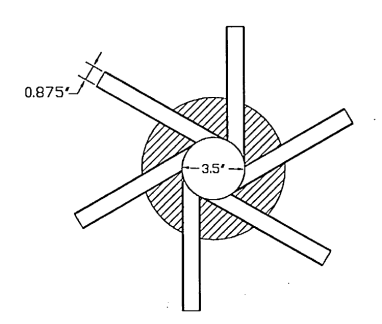
\includegraphics[width=0.4\textwidth]{tangentialinlet1.png}}
\subcaptionbox{Βάση διασταλτικής περιδίνησης \cite{1991_Legentilhomme}}
  [.5\linewidth]{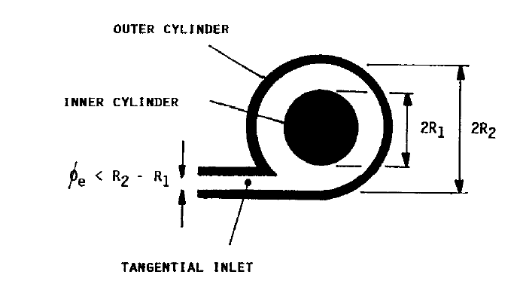
\includegraphics[width=0.5\textwidth]{tangentialinlet2.png}}
\caption{Περιδίνηση με χρήση βάσεων εφαπτομενικών εισόδων}\label{fig:tangin}
\end{figure}

Πολλά ερευνητικά έργα \parencites{1976_Murakami}{1975_Zaherzadeh}{1986_Morsi} έχουν χρησιμοποιήσει οδηγούς-πτερύγια. Αυτά ισαπέχουν γύρο από την είσοδο της εγκατάστασης και προσδίδουν εφαπτομενική ταχύτητα στη ροή (\prettyref{fig:gvanes}). Η ισχύς της συνιστώσας στροβιλισμού μπορεί να μεταβληθεί ρυθμίζοντας τη γωνία των πτερυγίων και η ομοιομορφία του πεδίου ροής μπορεί επίσης να βελτιωθεί με την αύξηση του αριθμού των πτερυγίων.

\begin{figure}[htbp]
\centering
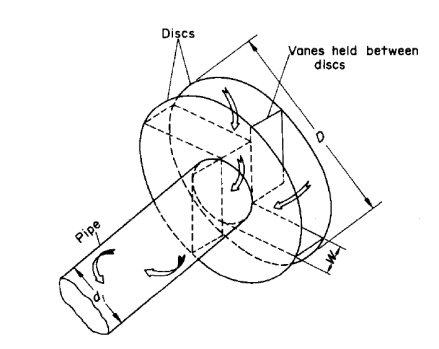
\includegraphics[scale=1]{guidedvanes.png}
\caption{Βάση περιδίνησης χρησιμοποιώντας οδηγούς-πτερύγια \cite{1975_Zaherzadeh}}\label{fig:gvanes}
\end{figure}

Η τεχνική των περιστρεφόμενων τμημάτων \parencites{1976_Murakami}{1954_Talbot}{1976_Crane}, η οποία προκαλεί στροβιλισμό με αντίσταση τριβής από ένα περιστρεφόμενο τοίχωμα, δημιουργεί ασθενή στροβιλισμό εάν χρησιμοποιηθεί σε απλή κυλινδρική διατομή. Οι \citeauthor{1976_Murakami} \cite{1976_Murakami} χρησιμοποίησαν μια ακτινική πτερωτή η οποία περιστρεφόταν μαζί με τον σωλήνα και δημιουργούσε μια ισχυρή δίνη κατά μήκος της ροής. Στις δακτυλιοειδείς ροές, η δημιουργία στροβιλισμού από την περιστροφή των εσωτερικού και του εξωτερικού κυλίνδρων έχει μελετηθεί εκτενώς από τον \citeauthor{1935_Taylor} \cite{1935_Taylor} ο οποίος χρησιμοποίησε ένα σύστημα ομόκεντρων κυλίνδρων, με τον εσωτερικό να περιστρέφεται, για να διερευνήσει το πώς εξελίσσεται ο στροβιλισμός κατά μήκος του αγωγού.

Τούτων λεχθέντων, η μακράν πιο συνηθισμένη διάταξη παραγωγή στροβιλισμού είναι μέσω συστραμμένης ταινίας (twisted tape) (\prettyref{fig:twisttape}) \parencites{1976_Hong}{2021_Wang}{2001_Manglik}. Ταινίες, πλάτους ίσου με τη διάμετρο του σωλήνα, συστρέφονται γύρο από το διαμήκη άξονα και εισάγονται σε σωλήνα, αναγκάζοντας το εργαζόμενο μέσο να περιστρέφεται μαζί με την ταινία. Το πεδίο ροής που παράγεται από την ταινία είναι πολύ διαφορετικό από εκείνο των εφαπτομενικών μεθόδων στροβιλισμού. Για αρχή, η συστραμμένη ταινία διαιρεί τη ροή σε δύο μικρότερες ημικυκλικής διατομής, οπότε δεν μπορεί να χαρακτηριστεί ως αξονοσυμμετρική. Η αυξημένη βρεγμένη επιφάνεια προκαλεί ανάπτυξη οριακών στρωμάτων που διαταράσσουν το πεδίο ροής και αυξάνουν αισθητά τον συντελεστή τριβής. Έχουν παρατηρηθεί επίσης σημαντικές διακυμάνσεις στα χαρακτηριστικά μεταφοράς θερμότητας της ροής.

\begin{figure}[htbp]
\centering
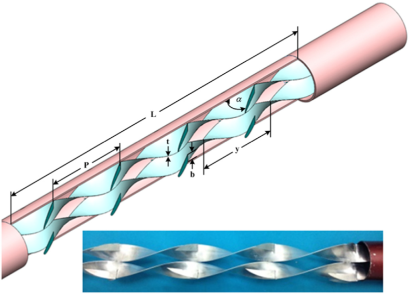
\includegraphics[scale=1]{twistedtape.png}
\caption{Δύο συστραμμένες ταινίες στην πειραματική διάταξη των \citeauthor{2016_Tamna} \cite{2016_Tamna}}\label{fig:twisttape}
\end{figure}

\section{Ποσοτικοποίηση στροβιλισμού}

\noindent Βασικό χαρακτηριστικό των περιδινούμενων ροών, που δημιουργούνται μέσω κάποιας διάταξης τοποθετημένης στην αρχή της ροής, είναι η εξασθένιση του στροβιλισμού κατά μήκος της διαδρομής της ροής λόγω της μείωσης της γωνιακής συνιστώσας της ταχύτητας. Ο συνήθης τρόπος ποσοτικοποίησης της στροβιλότητας είναι ο αριθμός στροβιλισμού (swirl number) \parencites{1984_Gupta_BOOK}{1998_FariasNeto}. Συμβολίζεται με το γράμμα S και είναι ο λόγος της εφαποτμενικής προς την αξονική ορμή:

\begin{equation}\label{eq:swirl}
S = \displaystyle\frac{\displaystyle\int_{0}^{R} u_z u_{\theta} r^2 \, dr}{R\displaystyle\int_{0}^{R} \left( u_z^2 - \frac{1}{2} u_{\theta}^2 \right)r \, dr}
\end{equation}

\noindent όπου $R$ η ακτίνα του αγωγού και $u_z,\, u_{\theta}$ η αξονική και η εφαπτομενική ταχύτητα για την ακτινική διεύθυνση αντίστοιχα.

\section{Θερμαινόμενες στροβιλώδεις ροές}

\noindent Οι πρώτες πειραματικές μελέτες που αξιοποίησαν διατάξεις δημιουργίας στροβιλισμό ο οποίος εξασθενεί κατά μήκος της ροής σωλήνα δακτυλιοειδούς διατομής είναι έξι στο σύνολό τους, όπως αναφέρει ο \citeauthor{1992_Solnordal_DISSERTATION} \cite{1992_Solnordal_DISSERTATION}. Όλες αυτές οι έρευνες προσδιόριζαν, μεταξύ άλλων, τον συντελεστή μετάδοσης θερμότητας των τοιχωμάτων του συστήματος κοιλοτήτων.

O τοπικός συντελεστής μεταφοράς θερμότητας, όπως αυτές έδειξαν, είναι συνυφασμένος με την απόσταση από τη γενέτειρα ροής $\left(x/d\right)$, τον αριθμό Reynolds $\left(Re\right)$, την ένταση στροβιλισμού $\left(S\right)$ και το πηλίκο θερμοκρασίας ρευστού προς την θερμοκρασία θερμαινόμενης επιφάνειας $\left(T_{\text{αντ}}/T_{\text{ρευ}}\right)$. Όλες αυτές οι μελέτες υπολόγισαν τον τοπικό αριθμό Nusselt και εν συνεχεία άλλαζαν τις προαναφερθείσες παραμέτρους προσπαθώντας να εξάγουν μια συσχέτιση. Μια κοινή παρατήρηση ήταν ότι ο τοπικός συντελεστής συναγωγής αυξανόταν με αντίστοιχη αύξηση των αριθμού Reynolds και της έντασης στροβιλισμού \parencites{1970_Blackwelder}{1973_KlepperO._CONF}{1975_Hay}{1984_Prata}, ενώ οι \citeauthor{1973_KlepperO._CONF} \cite{1973_KlepperO._CONF} και \citeauthor{1970_Blackwelder} \cite{1970_Blackwelder} παρατήρησαν ότι ο αριθμός Nusselt αυξανόταν όσο μεγαλύτερη ήταν η θερμοκρασιακή διαφορά μεταξύ ρευστού και κοιλότητας.

\subsection{Βελτίωση μετάδοσης θερμότητας}

\noindent Σε όλες τις έρευνες βρέθηκε ότι ο τοπικός συντελεστής μεταφορά θερμότητας μειωνόταν εκθετικά \parencites{1970_Blackwelder}{1973_KlepperO._CONF}{1975_Hay}{1984_Prata}, πράγμα που σημαίνει ότι η ενίσχυση μετάδοσης θερμότητας ήταν άμεσα συνυφασμένη με τη γωνιακή συνιστώσα της διατμητικής τάση του τοιχώματος, και ως εκ τούτου, με τον αριθμό στροβιλισμού.

Ο \citeauthor{1970_Blackwelder} \cite{1970_Blackwelder} βρήκε ότι η ενίσχυση μετάδοσης θερμότητας άρχισε να μειώνεται σημαντικά σε μήκος 60 με 80 διαμέτρους κατάντη της γενέτειρας ροής της πειραματικής του διάταξης, για αριθμούς Reynolds μέχρι \num{90e+3}. Οι \citeauthor{1975_Hay} \cite{1975_Hay}, χρησιμοποιώντας μικρότερους αριθμούς Reynolds και περισσότερη ένταση στροβιλισμού, βρήκαν ότι η ενίσχυση μετάδοσης θερμότητας μειώθηκε γύρω στο \qty{25}{\percent} της αρχικής της τιμής, σε μήκος 17.5 διαμέτρων κατάντη της ροής. 

Οι \citeauthor{1975_Zaherzadeh} \cite{1975_Zaherzadeh} έδειξαν ότι η ενίσχυση μετάδοσης θερμότητας μπορούσε να φτάσει μέχρι και το \qty{80}{\percent}. Οι \citeauthor{1975_Hay} \cite{1975_Hay} και οι \citeauthor{1984_Prata} \cite{1984_Prata} υπολόγισαν ενίσχυση μετάδοσης θερμότητας της τάξεως του \qty{500}{\percent} στην έξοδο των γενετειρών στροβιλισμού τους. Αμφότερες μελέτες χρησιμοποίησαν ιδιαίτερα υψηλές τιμές στροβιλισμού.

Η εμπειρική σχέση των \citeauthor{1975_Hay} \cite{1975_Hay} ήταν συναρτήσει του αριθμού στροβιλισμού, S (\prettyref{eq:hay}). Αυτή η συσχέτιση περιγράφει τα δεδομένα τους με ακρίβεια \qty{\pm 40}{\percent}. Αν και η αβεβαιότητα ήταν εκτός αποδεκτών ορίων (όπως καλή ώρα και τα δικά μας αποτελέσματα αργότερα), είναι λογικό δεδομένης της απλοϊκότητας του μοντέλου:
 
\begin{equation}\label{eq:hay}
\displaystyle\frac{Nu}{Nu_{ax}} = \left(S + 1\right)^{1.75}
\end{equation}

\noindent Οι \citeauthor{1970_Blackwelder} \cite{1970_Blackwelder} και \citeauthor{1973_KlepperO._CONF} \cite{1973_KlepperO._CONF} βρήκαν ότι οι τοπικοί συντελεστές συναγωγής ήταν συνυφασμένοι με την θερμοκρασιακή διαφορά ρευστού και τοιχώματος. Αμφότεροι χρησιμοποίησαν ιδιαίτερα υψηλές τιμές ροής θερμότητας, εντείνοντας την θερμοκρασιακή διαφορά. O διάταξη του \citeauthor{1970_Blackwelder} είχε $T_{\text{αντ}}/Τ_{\text{ρευ}} \le 2.1$ ενώ αυτή του \citeauthor{1973_KlepperO._CONF}, $T_{\text{αντ}}/Τ_{\text{ρευ}} = 1.5$.

Επιπλέον, ο \citeauthor{1970_Blackwelder} \cite{1970_Blackwelder} εφήρμοσε γραμμική παλινδρόμηση στα δεδομένα του, για συγκεκριμένο αριθμό Reynolds, χρησιμοποιώντας:

\begin{equation}\label{black}
\displaystyle\frac{Nu}{Nu_{ax}}\left(\displaystyle\frac{T_{\text{αντ}}}{T_{\text{ρευ}}} \right)^{A\frac{x}{d}} \quad \text{με} \quad \displaystyle\frac{x}{d}
\end{equation}

\noindent όπου Α σταθερά που εξαρτάται από την κλίση της συστραμμένης ταινίας. Για αξονικές ροές, ο \citeauthor{1973_KlepperO._CONF} \cite{1973_KlepperO._CONF} συσχέτισε, για πλήρως αναπτυγμένη ροή, τον αριθμό Nusselt με μια τροποποιημένη εξίσωση των \citeauthor{1930_Dittus} \cite{1930_Dittus}:

\begin{equation}\label{eq:dittus}
Nu_{ax} = 0.023 Re^{0.8} Pr^{0.4} \left(\displaystyle\frac{T_{\text{αντ}}}{T_{\text{ρευ}}}\right) ^ {-0.5}
\end{equation}

\noindent Τροποποιώντας την έκφραση αυτή, εξήγαγαν συσχέτιση για τους τοπικούς Nusselt σε περιδινούμενη ροή που φθίνει:

\begin{align}\label{eq:klepp}
Nu_{ax} &= 0.023 Re^{0.8} Pr^{0.4} \left(\displaystyle\frac{T_{\text{αντ}}}{T_{\text{ρευ}}}\right) ^ {-0.5} a b\\[2pt]
a &= \displaystyle\frac{0.7 + 4.2x \num{e-5}Re}{1 + 3.9x \num{e-5}Re}\nonumber\\[2pt]
b &= 1 + \displaystyle\frac{1.05}{\left\{0.5\frac{p}{d_o} + 1.25x\num{e-3}\frac{p}{d_o}\left( \frac{x}{d_o} \right)^2 \right\}^{0.6}}\nonumber
\end{align}

\noindent όπου ο όρος $a$ ισχύει για εύρη Reynolds \num{20e+3} με \num{380e+3} και ο όρος $p$ είναι η περίμετρος της συστραμμένης ταινίας. Τα δεδομένα του \citeauthor{1973_KlepperO._CONF} προσεγγίζονται από την ανωτέρω συσχέτιση με ακρίβεια \qty{\pm 10}{\percent}.

Να σημειωθεί εδώ ότι τα πειραματικά δεδομένα του \citeauthor{1973_KlepperO._CONF} ήταν πάρα πολλά, εκατοντάδες, και κάλυπταν ένα ευρύ φάσμα παραμέτρων (Re από \num{20e+3} μεχρι \num{380e+3}, $p/d_o$ από 4.76 μέχρι 8.05, $T_{\text{αντ}}/T_{\text{ρευ}}$ από 1 μέχρι 2.1). Τα δεδομένα του \citeauthor{1973_KlepperO._CONF} φαίνεται να συμφωνούν με αυτά άλλων δημοσιεύσεων, οπότε η εξίσωση αυτή είναι μια καλή προσέγγιση για περιδινούμενες ροές με χρήση συστραμμένων ταινιών.

Η προσέγγιση των \citeauthor{1971_Narezhnyy} \cite{1971_Narezhnyy} ήταν λίγο διαφορετική. Επειδή τα οριακά στρώματα εξελίσσονται κατά μήκος του σωλήνα, έκριναν πως η συσχέτιση μεταξύ των αριθμών Nusselt και Reynolds θα εξαρτιόταν από την εκάστοτε απόσταση των γενετειρών στροβιλισμού.

Παρατηρώντας τους τοπικούς Nusselt, $Nu_x$, να μεταβάλλονται αναλογικά με ${Re}_x^{0.8}$ όπως στην εξίσωση Dittus-Boelter \cite{1930_Dittus}, προσπάθησαν να βρούνε μια συσχέτιση της μορφής:

\begin{equation}\label{eq:dittuss}
Nu_x = c Re_x^{0.8}
\end{equation}

\noindent όπου η σταθερά c θεωρήθηκε ότι εξαρτιόταν της απόσταση, κατά μήκος της διάταξης, από την γενέτειρα στροβιλισμού και γωνίας εισροής ρευστού. Προσπαθώντας να προσαρμόσουν λοιπόν τα δεδομένα σε αυτού του είδους την εξίσωση κατέληξαν:

\begin{equation}
Nu_x = c_{ax} \left( 1 + tan \phi \right) ^ {0.8 exp\left( -0.0027\frac{x}{d_o} \right)} Re_x^{0.8}
\end{equation}

\noindent η ανωτέρω εξίσωση είναι εφαρμόσιμη για εύρη τοπικών Reynolds από \num{8e+4} με \num{e+7}, $\phi \le \ang{75}$, και $x/d_o \le 150$, ενώ η ακρίβεια της κυμαίνεται στο \qty{\pm 25}{\percent}.

\subsection{Πεδίο ροής}

\noindent Ένα σημαντικό χαρακτηριστικό των διατάξεων με στροβιλισμό έγκειται, όπως και αναφέρθηκε πιο πάνω, στο πολύπλοκο πεδίο ροής που δημιουργείται λόγω μίας κεντρικής ζώνης ανακυκλοφορίας \cite{2003_AlAbdeli}.

\noindent Μία από τις πρώτες προσπάθειες διερεύνησης του πεδίου ροής περιδινούμενων ροών που φθίνουν έγινε από τους \citeauthor{1961_Nissan} \cite{1961_Nissan}. Αυτοί μελέτησαν πειραματικά σωλήνα δακτυλιοειδούς διατομής όπου η περιδίνηση δημιουργείτο από δύο, αντίθετα τοποθετημένες, εφαπτομενικές εισόδους. Παρατήρησαν ότι το πεδίο ταχύτητας χωριζόταν σε τρεις διαφορετικές ζώνες ανάλογα τη μορφολογία του: (i) κοντά στον άξονα, η γωνιακή συνιστώσα της ταχύτητας αυξανόταν με την απομάκρυνση από τον άξονα, ενώ η αξονική γινόταν αρνητική, το οποίο υποδηλώνει την ύπαρξη αντιστρεπτής ροής, (ii) με την απομάκρυνση από τον άξονα υπήρξε αύξηση της γωνιακής ταχύτητας ενώ μηδενιζόταν η αξονική - εδώ, κοντά στον άξονα, υπάρχει πάλι αντιστροφή ροής και τέλος (iii) κοντά στο τοίχωμα, η γωνιακή ταχύτητα μειωνόταν απότομα ενώ η αξονική αυξανόταν. Η αποτύπωση των ζωνών ταχύτητας φαίνεται στο \prettyref{fig:nissan}.

\begin{figure}[htbp]
\centering
\subimport{Chapter2/Figs/pdftex}{nissan.pdf_tex}
\caption[Ζώνες πεδίου ταχύτητας περιδινούμενων ροών]{Οι τρεις διαφορετικές ζώνες ταχυτήτων που δημιουργούνται από στροβιλισμό σε σωλήνα \cite{1961_Nissan}. Οι συνεχείς γραμμές απεικονίζουν την κατανομή πίεσης στην αξονική απόσταση z, ενώ οι διακεκομμένες την κατανομή πίεσης στην απειροστή μεταβολή z + dz.}\label{fig:nissan}
\end{figure}

Επιπλέον, σε μια δακτυλιοειδή περιδινούμενη ροή που προκαλείται με τη βοήθεια οδηγών πτερυγίων, οι \citeauthor{1986_Morsi} \cite{1986_Morsi} έδειξαν ότι το εφαπτομενικό προφίλ ταχύτητας μοιάζει με αυτό εξαναγκασμένης δίνης η οποία τείνει προς το εσωτερικό τοίχωμα και φαίνεται να μειώνεται γραμμικά ενώ πλησιάζει τον εξωτερικό κύλινδρο. Αναλυτικότερα: η αξονική συνιστώσα της ταχύτητας φαινόταν να ακολουθεί ροή περιδίνησης, αλλά μεταβαλλόταν ριζικά κατά μήκος της διαδρομής της. Υψηλότερες αξονικές ταχύτητες εντοπίστηκαν κοντά στον εσωτερικό κύλινδρο, και αυτές φαίνονταν να μειώνονται με τη αύξηση της αξονικής απόστασης από το τμήμα εισόδου του δακτυλίου. Αυτά τα δεδομένα επιβεβαιώθηκαν πειραματικά και από τους \citeauthor{1991_Bottaro} \cite{1991_Bottaro} για ίδια διάταξη και συνθήκες στρωτής ροής, όπου η έγχυση ρευστού γινόταν μέσω μίας εφαπτομενικής εισόδου, καθώς επίσης και από τους \citeauthor{1990_Khodadadi} \cite{1990_Khodadadi}, οι οποίοι έκαναν ακριβώς τις ίδιες παρατηρήσεις, για παρόμοια διάταξη, σε συνθήκες τυρβώδους ροής.

\section{Στόχος παρούσας εργασίας}

\noindent Στην παρούσα εργασία, για την πειραματική διερεύνηση της βελτίωσης μετάδοσης θερμότητας, χρησιμοποιήθηκε στροβιλισμός σε σωλήνα δακτυλιοειδούς διατομής, ο οποίος εξασθενεί όσο εξελίσσεται η ροή. Η εν λόγω ροή δημιουργείτο από ειδικά διαμορφωμένες βάσεις που φέρουν εφαπτομενικές εισόδους ροής και είναι τοποθετημένες ανάντη της διάταξης -  παρόμοια με αυτή των \citeauthor{1995_Chang} \cite{1995_Chang}. Επίσης, ο λόγος πάχους του δακτυλίου που σχηματίζουν οι ομόκεντροι κύλινδροι, $\left(R_{\text{εξ.}} - R_{\text{εσ.}}\right)$, ισούται με τη διάμετρο των βρόγχων, $\left(D_{\beta}\right)$, ώστε να εξασφαλίζονται συνθήκες ροής "pure swirl flow" \cite{1991_Legentilhomme}.

Αυτού του είδος η διάταξη ήταν σχετικά εύκολο να σχεδιαστεί και να συντηρηθεί διότι δεν περιλάμβανε κινητά μέρη - όπως περιστρεφόμενους κυλίνδρους - και προκαλεί εν γένει ασθενέστερη πτώση πίεσης σε σύγκριση με τη μέθοδο οδηγών πτερυγίων. Επιπλέον η χρήση της εφαπτομενικής εισόδου καθιστά εύκολη την στεγανοποίηση της διάταξης. Το κύριο μειονέκτημα αυτών των ροών, ωστόσο, είναι ότι η ροή εξελίσσεται κατά μήκος της διαδρομής με φθίνοντα ρυθμό, όπου και παρατηρείται μείωση των συντελεστών μεταφοράς \parencites{1990_Legentilhomme}{1991_Legentilhomme}{1985_Shoukry}.

Για την ποσοτικοποίηση της βελτίωσης μετάδοσης θερμότητας, αναγκαία ήταν η χρήση συσχέτισης $\overline{Nu} = f(Re)$ για τον προσδιορισμό των αντιπροσωπευτικών Nusselt (βλ. υποενότητα \ref{repnu}). Για τον σκοπό αυτό χρησιμοποιήθηκε η πιο απλή από τις προαναφερθείσες συσχετίσεις, μια παρόμοια αυτής των Dittus-Boelter \cite{1930_Dittus}. Η αποτίμηση της επιλογής αυτής θα γίνει με το πέρας των υπολογισμών, όπου θα έχει προηγηθεί στατιστική ανάλυση, και θα φανεί η αβεβαιότητα στα τελικά αποτελέσματα.
%!TEX root = ../thesis.tex
%*******************************************************************************
%****************************** Third Chapter **********************************
%*******************************************************************************
\chapter{Εγκατάσταση δοκιμών}\label{ch:experiment}

\begin{chapquote}{Richard Feynman\footnote{Αυτό έχει ειπωθεί στις διαλέξεις του Feynman στο Cornell, το 1964. Κομμάτι των διαλέξεων αυτών είναι διαθέσιμο στο σύνδεσμο \href{https://youtu.be/OL6-x0modwY}{https://youtu.be/OL6-x0modwY}. Ένα πιο πλήρες κείμενο μπορεί να βρεθεί στον ιστότοπο του \citeauthor{Pomeroy2012} \cite{Pomeroy2012}.}}
“It doesn’t matter how beautiful your theory is, it doesn’t matter how smart you are.
If it doesn’t agree with experiment, it’s wrong.”
\end{chapquote}

% **************************** Define Graphics Path **************************
\ifpdf
    \graphicspath{{Chapter3/Figs/Raster/}{Chapter3/Figs/PDF/}{Chapter3/Figs/}}
\else
    \graphicspath{{Chapter3/Figs/Vector/}{Chapter3/Figs/}}
\fi


% ******************************* Nomenclature ****************************************

\nomenclature[a-$z/L$]{$z/L$}{ανηγμένο μήκος αντίστασης (εσωτερικού κυλίνδρου)}

\noindent Στο κεφάλαιο αυτό περιγράφεται η πειραματική διάταξη που κατασκευάστηκε για την διερεύνηση της ενίσχυσης μετάδοσης θερμότητας περιδινούμενων ροών. Περιγράφονται επίσης οι πειραματικές συσκευές και τα χρησιμοποιηθέντα μετρητικά όργανα, και γίνεται αναφορά στην πειραματική διαδικασία λήψης μετρήσεων.

\section{Πειραματική διάταξη}

\noindent Σκαρίφημα της πειραματικής διάταξης απεικονίζεται στο \prettyref{fig:schematic}. Πρόκειται για σύστημα που απαρτίζεται από (i) τη βάση ροής, (ii) τη διάταξη ομόκεντρων κυλίνδρων και (iii) από έναν ανεμιστήρα αναρρόφησης. Η σχεδίαση των ομόκεντρων κυλίνδρων και βάσεων βρόγχων ήταν τέτοια ώστε ο λόγος πάχους του δακτυλίου των πρώτων $\left(R_{\text{εξ.}} - R_{\text{εσ.}}\right)$ με τη διάμετρο των βρόγχων $\left(D_{\beta}\right)$ να είναι 1:1. Έτσι εξασφαλίζονται συνθήκες ροής "pure swirl flow" \cite{1991_Legentilhomme}. Οι βάσεις ροής ήταν τοποθετημένες ανάντη της διάταξης ενώ ο ανεμιστήρας αναρρόφησης κατάντη της, και ήταν ικανός να παρέχει ταχύτητες μέχρι και \qty{2}{\metre\per\second} στην έξοδο της διάταξης. 

\clearpage

\begin{figure}[tbp]
\centering
\subimport{Chapter3/Figs/pdftex}{schematic.pdf_tex}
\caption{Σκαρίφημα πειραματικής διάταξης}\label{fig:schematic}
\end{figure}

\subsection{Βάσεις ροής}

\noindent Όπως φαίνεται στο \prettyref{fig:swirlgenerators}, οι βάσεις ροής ήταν πέντε στο σύνολό τους: μία βάση αξονικής και τέσσερις περιδινούμενης ροής. Οι βάσεις περιδινούμενης (θα αναφέρονται στο κείμενο και ως βάσεις βρόγχων) είχαν συμμετρικά τέσσερις βρόγχους στην περιφέρειά τους, με κλίση $\left(\phi\right)$ σε σχέση με την εγκάρσια διατομή τους. Όλες εκτυπώθηκαν με τριδιάστατο εκτυπωτή και είναι κατασκευασμένες από υλικό με αντοχή σε θερμικά φορτία μέχρι \qty{150}{\degreeCelsius}. Σχεδιάστηκαν με τρόπο τέτοιο ώστε να γίνεται καλή εφαρμογή με το σύστημα κυλίνδρων, ενώ στη βάση τους υπάρχει μια μικρή οπή για τη διέλευση των θερμοστοιχείων που είναι τοποθετημένα στον εσωτερικό κύλινδρο. Περιδίνηση ροής δημιουργείται εφαρμόζοντας την κατάλληλη βάση, η οποία εισάγει εφαπτομενικό ρεύμα αέρα και ψύχει τον εσωτερικό κύλινδρο ο οποίος θερμαίνεται.

\clearpage

\begin{figure}[tbp]
\centering
\subimport{Chapter3/Figs/pdftex}{swirlGenerators.pdf_tex}
\caption{Βάσεις ροής}\label{fig:swirlgenerators}
\end{figure}

\subsection{Διάταξη ομόκεντρων κυλίνδρων}

\noindent Το βασικό κομμάτι της εγκατάστασης αποτελείται από δύο ομόκεντρους κυλίνδρους, τον εσωτερικό (ή αντίσταση) και εξωτερικό, στο διάκενο των οποίων ρέει το ρευστό. Η διάταξη των ομόκεντρων κυλίνδρων φαίνεται στο \prettyref{fig:concylinders}.


\begin{figure}[htbp]
\centering
\subimport{Chapter3/Figs/pdftex}{concylinders.pdf_tex}
\caption{Σύστημα ομόκεντρων κυλίνδρων: (α) Εξωτερικός (β) Εσωτερικός}\label{fig:concylinders}
\end{figure}
	
 
\subsubsection{Εξωτερικός κύλινδρος}

\noindent Ως εξωτερικός κύλινδρος χρησιμοποιήθηκε σωλήνας Plexiglass εσωτερικής διαμέτρου \qty{40}{\milli\metre} με πάχος \qty{5}{\milli\metre} και μήκος \qty{895}{\milli\metre}. Η επιλογή του υλικού ήταν τέτοια ώστε να διευκολύνεται η περαιτέρω κατεργασία του, σε περίπτωση που αυτή χρειαζόταν, και οι μηχανικές του ιδιότητες να συνδράμουν στην ομαλή διεξαγωγή των πειραμάτων - το υλικό έχει χαμηλό συντελεστή θερμικής αγωγιμότητας και είναι διαφανές.

Υλικό ανακλώμενης επιφάνειας τυλίχτηκε γύρω από τον εξωτερικό κύλινδρο, ώστε να περιοριστούν οι απώλειες θερμότητας λόγω ακτινοβολίας από τον εσωτερικό προς τον εξωτερικό κύλινδρο. Προστέθηκε επίσης άλλη μια στρώση μονωτικού υλικού προς μείωση απωλειών λόγω αγωγής.

Τέλος, στην κορυφή του εξωτερικού κυλίνδρου, τοποθετήθηκαν τρεις κοχλίες $Μ14$ για να διασφαλιστεί η εκκεντρότητα του με τον εσωτερικό κύλινδρο και να μειωθούν, όσο αυτό ήταν εφικτό, τα χωρικά σφάλματα.

\subsubsection{Εσωτερικός κύλινδρος}

\noindent Για τη δημιουργία του εσωτερικού κυλίνδρου χρησιμοποιήθηκε σωλήνας διαμέτρου \qty{22}{\milli\metre}, πάχους \qty{1}{\milli\metre} και μήκους \qty{900}{\milli\metre}, με καλυμμένη τη μία του έξοδο, ανάντη του συστήματος. Εντός του σωλήνα τοποθετήθηκε κεραμικό υλικό, ανθεκτικό σε θερμικά φορτία, και περί αυτού τυλίχτηκε ομοιόμορφα σύρμα αντίστασης σε κατάλληλα σχηματισμένες αυλακώσεις, για τα επιτευχθεί όσο το δυνατόν πιο ομοιόμορφη θέρμανση. Κατά τη διάρκεια της τοποθέτησης του καλωδίου αντίστασης, δόθηκε ιδιαίτερη προσοχή στην αποφυγή περιτύλιξης για αποφυγή βραχυκύκλωσής του.

Η αντίσταση τροφοδοτείτο από σταθερή πηγή τάσης τύπου MERSAN, με ονομαστική τιμή \qty{50}{\volt}. Επειδή η τάση που διέπει το καλώδιο δεν πρέπει να μεταδοθεί στον χάλκινο σωλήνα, χρησιμοποιήθηκε μονωτική ταινία τύπου Mica η οποία είναι ηλεκτρικά καλός μονωτής και ταυτόχρονα θερμικά αγώγιμο υλικό. Η τοποθέτηση της ταινίας ήταν τέτοια ώστε να επικαλύπτει επακριβώς το διάκενο μεταξύ αυλακώσεων και τυλιγμένου σύρματος, και να βρίσκεται όσο το δυνατόν πλησιέστερα στο χάλκινο σωλήνα.

Για τον προσδιορισμό της θερμοκρασίας κατά μήκος της επιφάνειας του χάλκινου σωλήνα χρησιμοποιήθηκαν θερμοστοιχεία τύπου Κ, τοποθετημένα, με ομοιόμορφο μοτίβο, κατά μήκος της εσωτερικής επιφάνειάς του, με θερμικά αγώγιμη κόλλα. Επειδή τα θερμοστοιχεία τοποθετήθηκαν στο εσωτερικό του σωλήνα, για μην εμποδίσουν το πεδίο ροής, πακτώθηκαν στο κάτω άκρο της αντίστασης με σιλικόνη - θερμικά αγώγιμο υλικό μεν, ηλεκτρικά μονωτικό δε. Στο κάτω μέρος της αντίστασης τοποθετήθηκε κατάλληλη βάση ώστε να προσδένεται με τις βάσεις ροής, και η οποία αποτελείτο από PTFE, το οποίο έχει χαμηλό συντελεστή μετάδοσης θερμότητας και αντοχή σε υψηλά θερμικά φορτία.

\subsection{Ανεμιστήρας αναρρόφησης}

\noindent Στο πάνω μέρος της διάταξης τοποθετήθηκε ανεμιστήρας αναρρόφησης τύπου Corsair iCUE SP120, ονομαστικής τάσης \qty{24}{\volt}. Για τον έλεγχο της ροής, ο ανεμιστήρας συνδεόταν με πηγή συνεχούς ρεύματος EZ GP-4303D DC, ονομαστικής τάσης \qty{40}{\volt}. Για την εφαρμογή του ανεμιστήρα με τη διάταξη ομόκεντρων κυλίνδρων, αλλά και για την σύνδεσή του με τον μετρητή ογκομετρικής παροχής, δημιουργήθηκε ειδική θήκη. Η θήκη αυτή αποτελείτο από το ίδιο υλικό με αυτό των βάσεων ροής, και η ανοχή των διαστάσεών της δεν υπερέβαινε, σύμφωνα με τον κατασκευαστή τουλάχιστον, τα \qty{0.2}{\milli\metre}.

\section{Μετρητικά όργανα και ανάκτηση δεδομένων}

\noindent Για την πειραματική διερεύνηση της ενίσχυσης μετάδοσης θερμότητας στον εσωτερικό κύλινδρο, λήφθηκαν μετρήσεις θερμοκρασίας, χρόνου και τάσεως-έντασης ρεύματος. Οι πρώτες έγιναν με χρήση θερμοστοιχείων τύπου Κ, αυτές του χρόνου με συνδυασμό χρονομέτρου χειρός και μετρητή παροχής, και αυτές των τάσεων-έντασης ρεύματος με πολύμετρο ακριβείας. Οι μετρήσεις των θερμοκρασιών καταγράφονταν σε ηλεκτρονικό υπολογιστή, ενώ οι υπόλοιπες λήφθηκαν χειρωνακτικά. Η ανάλυση της πειραματικής αβεβαιότητας των μετρήσεων καθώς επίσης και των υπολογισθέντων μεγεθών, αναφέρονται στην υποενότητα~\ref{uncertaintyofmeasurements}.

\subsection{Θερμοστοιχεία τύπου Κ}

\noindent Για μετρήσεις θερμοκρασιών, χρησιμοποιήθηκαν θερμοστοιχεία τύπου Κ, τα οποία συγκολήθηκαν στο εργαστήριο λίγο πριν την τοποθέτησή τους στον εσωτερικό κύλινδρο. Στο σύνολό τους ήταν έντεκα: εννέα μετρούσαν τοπικές θερμοκρασίες κατά μήκος της αντίστασης, ένα κατάντη της διάταξης για την θερμοκρασία εισόδου του ρευστού και άλλο ένα ανάντη της διάτξης για μέτρηση της θερμοκρασίας εξόδου.

\begin{figure}[h!]
\centering
\subimport{Chapter3/Figs/pdftex}{thermocouples.pdf_tex}
\caption{Θέσεις θερμοστοιχείων της πειραματικής διάταξης}
\end{figure}

Για τη συνεχή καταγραφή της θερμοκρασίας, επί και εκτός της αντίστασης, χρησιμοποιήθηκε πολύμετρο τύπου KEITHLEY 2700. Δυστυχώς δεν κατέστη δυνατή η συνεχής αποθήκευση των δεδομένων αυτών λόγω \enquote{διαξιφισμού} λογισμικών πολυμέτρου-υπολογιστή. Ωστόσο, χρησιμοποιήθηκε επιτυχώς για τον συνεχή έλεγχο των θερμοκρασιών, μέχρι αυτές να συγκλίνουν προς μία σταθερή τιμή. 

Τα θερμοστοιχεία, εξαιτίας της σχετικά απλής χρήσης τους, αποτελούν την πλέον διαδεδομένη μέθοδο μέτρησης της θερμοκρασίας. Ωστόσο, οι μετρήσεις μπορούν να επηρεαστούν (και συνήθως επηρεάζονται) σημαντικά από απώλειες θερμότητας λόγω συναγωγής και της διαδικασίας συγκόλλησής τους. Οπότε οι μετρήσεις τείνουν να υπερεκτιμούνται αυτών των πραγματικών τιμών λόγω φαινομένων αδράνειας και ενεργειακών απωλειών \cite{1994_FluidDynamicsRhodeSaintGenese_BOOK}. Στην παρούσα εργασία, δεν έγινε καμία προσπάθεια αντιμετώπισης των σφαλμάτων αυτών.

\subsection{Μετρητής φυσικού αερίου}

\noindent Ο μετρητής φυσικού αερίου συνδέεται στην έξοδο του συγκροτήματος ανεμιστήρα. Χρησιμοποιήθηκε σε συνδυασμό με χρονόμετρο, όπου, σε κάθε πείραμα, καταγραφόταν ο απαιτούμενος χρόνος για τη διέλευση \qty{0.1}{\metre\cubed} αέρα. Όλες οι παροχές του αέρα, για κάθε διάταξη ροής, προέρχονται από τον ανεμιστήρα αναρρόφησης, οι στροφές του οποίου ρυθμίζονταν κάνοντας χρήση πηγής συνεχούς ρεύματος.

Λόγω παλαιότητάς του πραγματοποιήθηκε \enquote{σχετική βαθμονόμηση} με θερμό νήμα, ώστε να υπάρξει μια εκτίμηση για την εγκυρότητά του. Περισσότερες πληροφορίες για διαδικασία αναφέρονται στο \prettyref{app:calibration}.

\subsection{Ψηφιακό πολύμετρο}

\noindent Λόγω παλαιότητας των πηγών τάσεως, οι ενδείξεις των εγγενών ενδείξεών τους δεν ήταν αξιόπιστες. Κρίθηκε σκόπιμο λοιπόν να χρησιμοποιηθεί πολύμετρο ακριβείας τύπου DT-9205A, για τη μέτρηση των τιμών τάσης και έντασης ρεύματος του ανεμιστήρα και της αντίστασης.

\section{Διερευνηθείσες ροές και μεθοδολογία μετρήσεων}

\noindent Έχοντας συναρμολογήσει την όλη διάταξη, σε πρώτο στάδιο, ορίστηκαν οι συνθήκες λειτουργίας των πειραμάτων και η μεθοδολογία για την αξιολόγηση μετάδοσης θερμότητας των βάσεων περιδίνησης. Αποφασίστηκε ότι σε κάθε πειραματική διάταξη θα λαμβάνονται δεδομένα για τέσσερις αριθμούς Reynolds: 1100, 1400, 1700 και 2000 - εύρος που εξασφαλίζει συνθήκες στρωτής ροή για την εν λόγο διάταξη \cite{Dou2005}. Όλα τα μεγέθη ήταν χρονικά αμετάβλητα, δηλαδή επικρατούσαν συνθήκες μόνιμης ροής. Για να επιτευχθεί αυτό, υπήρξε συνεχής έλεγχος των ενδείξεων των θερμοστοιχείων μέχρι οι τιμές τους να συγκλίνουν προς μία σταθερή τιμή. Τέλος, για να μπορέσει να καταστεί δυνατή η σύγκριση μετάδοσης θερμότητας μεταξύ των διατάξεων, η ηλεκτρική τροφοδότηση του εσωτερικού κυλίνδρου ήταν η ίδια για όλα τα πειράματα \cite{1974_Bergles}, με ένταση ρεύματος \qty{0,63}{\ampere} και τάσης \qty{29.5}{\volt}, οι οποίες δίνουν την παρεχόμενη ηλεκτρική ισχύ της αντίστασης $\dot{Q}_{res.} = \qty{18.85}{\watt}$.

Έγιναν λοιπόν πειράματα, με όλους τους πιθανούς συνδυασμούς αριθμών $\left(\alpha\right)$ και κλίσης $\left(\phi\right)$ βρόγχων, για τέσσερις αριθμούς Reynolds. Επίσης, για το ίδιο εύρος Reynolds, έλαβαν χώρα άλλα τέσσερα πειράματα χρησιμοποιώντας τη διάταξη αξονικής ροής, ώστε να υπάρχουν τιμές αναφοράς για την ενίσχυση μετάδοσης θερμότητας. Στο σύνολό τους, τα πειράματα ήταν 68.

Τα πειράματα έλαβαν χώρα σε διάστημα δύο μηνών, τον Οκτώβριο και το Νοέμβριο του έτους 2019 . Για λόγους συνέπειας, τα πειράματα ξεκινούσαν τις πρωινές ώρες και ολοκληρώνονταν νωρίς το μεσημέρι της ίδιας ημέρας ώστε να μειωθεί η συνεισφορά του παράγοντα εξωτερικής θερμοκρασίας, η οποία αυξανόταν αισθητά το μεσημέρι. Πριν την εκκίνηση των πειραμάτων της ημέρας, κάθε φορά, παρατηρούνταν με σχολαστικότητα οι ενδείξεις των θερμοστοιχείων κατά μήκος του εσωτερικού κυλίνδρου. Αυτές θα έπρεπε πάντα να έχουν αύξουσα τιμή, διαβάζοντας τες ανάντη του κυλίνδρου, λόγο φυσικής κυκλοφορίας του αέρα.

Ιδιαίτερη προσοχή δόθηκε στην τοποθέτηση των συσκευών λήψης δεδομένων και των μετρητικών συστημάτων, ώστε να αποφευχθούν πιθανές μετακινήσεις και άσκοπες αποσυναρμολογήσεις την ώρα των πειραμάτων. Λάθη που σχετίζονται με την  ελλιπή πρόσδεση των κυλίνδρων, πιθανόν να δημιουργήσουν διαρροές, άρα και διαφορετικές συνθήκες ροής συγκριτικά με αυτές των υπολοίπων. Επιπλέον, τυχόν ανεπάρκεια στην ευθυγράμμιση των εσωτερικού και εξωτερικού κυλίνδρων είναι ικανή να επάγει ανεπιθύμητες αλλαγές στο πεδίο ροής, και να οδηγήσει σε λανθασμένες μετρήσεις. Γενικά δεν επιχειρήθηκε να αξιολογηθεί η αβεβαιότητα που σχετίζεται με την ανεπάρκεια ευθυγράμμισης (χωρικό σφάλμα). Κατά τη διάρκεια των πειραμάτων δεχτήκαμε, κατά σύμβαση, ότι οι ανοχές μεταξύ των προσδεμένων μερών, καθώς και η ευθυγράμμισή τους, ελεγχόταν αρκετά αποτελεσματικά, και ότι τυχόν αβεβαιότητες, που θα μπορούσαν να αποδοθούν σε κακή συνδεσμολογία, ήταν αμελητέες.

\subsubsection{Αποτελέσματα δοκιμών}

\noindent Τα πειραματικά αποτελέσματα καταγράφονται στο \prettyref{app:measurements}. Οι ληφθείσες μετρήσεις αξονικής ροής εμπεριέχονται όλες στον Πίνακα~\ref{axialmeas}. Ενώ οι μετρήσεις περιδινούμενων ροών, λόγω αυξημένου όγκου δεδομένων, εμπεριέχονται στις υπόλοιπες σελίδες. Συγκεκριμένα: οι μετρήσεις θερμοκρασίας βρίσκονται στους Πίνακες~\ref{tempmeas45-60}-\ref{tempmeas75-90}, οι μετρήσεις τάσης και έντασης ρεύματος του ανεμιστήρα στον Πίνακα~\ref{tab:flowmeas} και τέλος, οι μετρήσεις χρόνου για τη διέλευση \qty{0.1}{\metre\cubed} αέρα, στον Πίνακα~\ref{tab:flowmeas}.

Στο επόμενο κεφάλαιο θα παρουσιαστούν η ανάλυση δεδομένων καθώς επίσης και η εκτιμόμενη αβεβαιότητα των μετρητικών οργάνων και των υπολογισθέντων μεγεθών.
%!TEX root = ../thesis.tex
%*******************************************************************************
%****************************** Fourth Chapter **********************************
%*******************************************************************************
\chapter{Yπολογισμοί και ανάλυση αβεβαιότητας}\label{ch:uncertaintyanalysis}

\begin{chapquote}{Winston Churchill}
“True genius resides in the capacity for evaluation of uncertain, hazardous, and conflicting
information.”
\end{chapquote}


% **************************** Define Graphics Path **************************
\ifpdf
    \graphicspath{{Chapter4/Figs/Raster/}{Chapter4/Figs/PDF/}{Chapter4/Figs/}}
\else
    \graphicspath{{Chapter4/Figs/Vector/}{Chapter4/Figs/}}
\fi


% ******************************* Nomenclature ****************************************
\nomenclature[a-$Re$]{$Re$}{Αριθμός Reynolds}
\nomenclature[a-$Nu$]{$Nu$}{Αριθμός Nusselt}
\nomenclature[a-$Bi$]{$Bi$}{Αριθμός Biot}
\nomenclature[a-$h$]{$h$}{Συντελεστής θερμικής συναγωγιμότητας, \unit{\watt\per\metre\squared\per\kelvin}}
\nomenclature[a-$\overline{Nu}$]{$\overline{Nu}$}{Μέσος αριθμός Nusselt}
\nomenclature[a-$\overline{Nu}_{\scriptsize{avg}}$]{$\overline{Nu}_{\scriptsize{avg}}$}{Αντιπροσωπευτικός αριθμός Nusselt}
\nomenclature[a-$Pr$]{$Pr$}{Αριθμός Prandtl}
\nomenclature[a-$J$]{$J$}{Ιακωβιανός πίνακας}
\nomenclature[a-\volume]{\volume}{Όγκος, \unit{\metre\cubed}}
\nomenclature[a-$\dot{\volume}$]{$\dot{\volume}$}{Ογκομετρική παροχή, \unit{\metre\cubed\per\second}}
\nomenclature[a-$\dot{Q}_{sys.}$]{$\dot{Q}_{sys.}$}{Ροή θερμότητας προς τον αέρα, \unit{\joule\per\second}}
\nomenclature[a-$\dot{W}$]{$\dot{W}$}{Παρεχόμενη ηλεκτρική ισχύς ανεμιστήρα, \unit{\joule\per\second}}
\nomenclature[a-$\dot{W}_{\scriptsize{avg}}$]{$\dot{W}_{\scriptsize{avg}}$}{Αντιπροσωπευτική ηλεκτρική ισχύς ανεμιστήρα, \unit{\joule\per\second}}
\nomenclature[a-$\dot{Q}_{res.}$]{$\dot{Q}_{res.}$}{Παρεχόμενη ηλεκτρική ισχύς στην αντίσταση, \unit{\joule\per\second}}
\nomenclature[a-$A_{heated}$]{$A_{heated}$}{Εμβαδόν θερμαινόμενης επιφάνειας, \unit{\metre\squared}}
\nomenclature[a-$\dot{q}_{conv.}$]{$\dot{q}_{conv.}$}{Ροή θερμικής ενέργειας στην αντίσταση, \unit{\joule\per\second\per\metre\squared}}
\nomenclature[a-$V_{\text{ανεμ.}}$]{$V_{\text{ανεμ.}}$}{Τάση τροφοδοσίας ανεμιστήρα, \unit{\volt}}
\nomenclature[a-$I_{\text{ανεμ.}}$]{$I_{\text{ανεμ.}}$}{Ένταση ρεύματος τροφοδοσίας ανεμιστήρα, \unit{\ampere}}
\nomenclature[a-$Τ_{mean}$]{$Τ_{mean}$}{Μέση θερμοκρασία διάταξης, \unit{\degreeCelsius}}
\nomenclature[a-$Τ_{\sigma}$]{$Τ_{\sigma}$}{Τυπική απόκλιση θερμοκρασίας, \unit{\degreeCelsius}}
\nomenclature[a-$w_x$]{$w_x$}{Βάρος εκάστοτε δεδομένων}
\nomenclature[a-$s^2$]{$s^2$}{Διασπορά εκάστοτε δεδομένων}
\nomenclature[a-$A_{ann.}$]{$A_{ann.}$}{Εμβαδόν διατομής δακτυλιοειδούς σωλήνα, \unit{\metre\squared}}
\nomenclature[a-$\overline{U}$]{$\overline{U}$}{Μέση ταχύτητα, \unit{\metre\per\second}}
\nomenclature[a-$C_p$]{$C_p$}{Ειδική θερμοχωρητικότητα, \unit{\kilo\joule\per\kilogram\per\kelvin}}
\nomenclature[a-$\dot{m}$]{$\dot{m}$}{Παροχή μάζας, \unit{\kilogram\per\second}}
\nomenclature[a-$D_\beta$]{$D_\beta$}{Διάμετρος οπής βρόγχου, \unit{\metre}}
\nomenclature[a-$D_{\text{εξ.}}$]{$D_{\text{εξ.}}$}{Διάμετρος εξωτερικού κυλίνδρου, \unit{\metre}}
\nomenclature[a-$R_{\text{εξ.}}$]{$R_{\text{εξ.}}$}{Ακτίνα εξωτερικού κυλίνδρου, \unit{\metre}}
\nomenclature[a-$D_{\text{εσ.}}$]{$D_{\text{εσ.}}$}{Διάμετρος εσωτερικού κυλίνδρου, \unit{\metre}}
\nomenclature[a-$R_{\text{εσ.}}$]{$R_{\text{εσ.}}$}{Ακτίνα εσωτερικού κυλίνδρου, \unit{\metre}}
\nomenclature[a-$\left\langle \overline{X} \right\rangle$]{$\left\langle \overline{X} \right\rangle$}{Ομαδοποιημένος μέσος όρος}
\nomenclature[a-$p$]{$p$}{Περίμετρος συστραμμένης ταινίας, m}

\nomenclature[z-RSS]{RSS}{Root-Sum-Squared}
\nomenclature[z-DRE]{DRE}{Data Reduction Equation}

\nomenclature[s-$\chi$]{x}{Θέση θερμοστοιχείων κατά μήκος της αντίστασης, \unit{\metre}}
\nomenclature[s-x, y, z]{x, y, x}{Καρτεσιανές συνιστώσες, \unit{\metre}}
\nomenclature[s-r, θ, z]{r, θ, z}{Κυλινδρικές συνιστώσες}
\nomenclature[s-ρευ.]{ρευ.}{ρευστού}

\nomenclature[g-$\delta$]{$\delta$}{Πάχος οριακού στρώματος, \unit{\metre}}
\nomenclature[g-$\rho$]{$\rho$}{Πυκνότητα, \unit{\kilogram\per\meter\cubed}}
\nomenclature[g-$\kappa$]{$\kappa$}{Θερμική αγωγιμότητα, \unit{\watt\per\metre\per\kelvin}}
\nomenclature[g-$\mu$]{$\mu$}{Δυναμικό ιξώδες, \unit{\kilogram\per\meter\per\second}}
\nomenclature[g-$\left\langle\sigma _X\right\rangle$]{$\left\langle\sigma _X\right\rangle$}{Ομαδοποιημένη τυπική απόκλιση}
\nomenclature[g-$\left\langle\sigma _{\overline{X}}\right\rangle$]{$\left\langle\sigma _{\overline{X}}\right\rangle$}{Ομαδοποιημένη τυπική απόκλιση των μέσων}
\nomenclature[g-$\delta X_{0}$]{$\delta X_{0}$}{Σφάλμα μηδενικής τάξης}
\nomenclature[g-$\delta X_{1}$]{$\delta X_{1}$}{Σφάλμα πρώτης τάξης}
\nomenclature[g-$\delta X_{N}$]{$\delta X_{N}$}{Σφάλμα $N^{\text{ής}}$ τάξης}
\nomenclature[g-$\delta X_{sens.}$]{$\delta X_{sens.}$}{Σφάλμα ευαισθησίας}

\nomenclature[x-$\nabla$]{$\nabla$}{Τελεστής Euler}

\noindent Στο κεφάλαιο αυτό περιγράφεται η αναλυτική μεθοδολογία που αναπτύχθηκε για τη θερμοδυναμική διερεύνηση όλων των διατάξεων ροών ομόκεντρων κυλίνδρων (περιδινούμενων και αξονικών). Συγκεκριμένα: (i) αναφέρεται η ανάλυση δεδομένων καθώς και οι υποθέσεις στις οποίες αυτή βασίστηκε, (ii) παρουσιάζεται λεπτομερώς η ανάλυση αβεβαιότητας των μετρούμενων τιμών, και η συνεισφορά αυτών στα τελικά αποτελέσματα και (iii) παρουσιάζονται οι σχετικές αβεβαιότητες που θα έχουν τα αποτελέσματα των αναλυτικών υπολογισμών για τα εύρη λειτουργίας στα οποία ελήφθησαν οι πειραματικές μετρήσεις.

Ο συγγραφέας οφείλει να ομολογήσει σε αυτό το σημείο ότι ο τρόπος συγγραφής του παρόντος κεφαλαίου συνιστά πλεονασμό. Πράγματι, πειραματικής φύσεως διατριβές \parencites{2015_Μηλιδόνης_DISSERTATION}{2020_Δόγκας_DISSERTATION} είθισται να αναφέρονται στην ανάλυση αβεβαιότητας περιληπτικά, συμπεριλαμβάνοντας επιμέρους επεξηγήσεις στα παραρτήματα. Ωστόσο, επειδή η αρχική πρόθεση του συγγραφέα ήταν να στήσει ένα αρκετά στιβαρό πείραμα, αξιοποιώντας ό,τι εργαλεία είχε στη διάθεση του, και επειδή ο περισσότερος φόρτος εργασίας (υλοποίηση κώδικα, αναλυτικοί υπολογισμοί, ανασκόπηση βιβλιογραφίας κλπ.) καταναλώθηκε για τον σκοπό αυτό, αποφάσισε να συντάξει το παρών κεφάλαιο με λίγες παραπάνω κουβέντες.

\section{Παραδοχές και ανάλυση δεδομένων}

\noindent Κύριος στόχος των πειραματικών μετρήσεων ήταν ο προσδιορισμός του τοπικού αδιάστατου αριθμού Nusselt, $\overline{Nu}$, κατά μήκος του όγκου ελέγχου του συστήματος, δηλαδή στην περιοχή που περιβάλλεται από τον εξωτερικό και εσωτερικό κύλινδρο. Με αυτό ως γνώμονα, αναπτύχθηκε αναλυτική μεθοδολογία προσδιορισμού των σχετικών μεγεθών, βασισμένη σε ορισμένες παραδοχές που αφορούν (i) το πεδίο ροής και (ii) την πειραματική διάταξη.

Οι προϋποθέσεις που πρέπει να ικανοποιούνται στο πεδίο ροής είναι οι εξής:

\begin{itemize}
\item Το εργαζόμενο μέσο είναι αέρας και εισέρχεται στην διάταξη με θερμοκρασία ίση με αυτή του περιβάλλοντος.
\item Το εργαζόμενο μέσο είναι Νευτωνικό ρευστό και συμπεριφέρεται ως ιδανικό αέριο.
\item H θερμοκρασία του αέρα, μεταξύ εισόδου και εξόδου της διάταξης, συμβαίνει γραμμικά. Η παραδοχή αυτή είναι συνήθης σε ροές κυκλικών διατομών για οριακές συνθήκες σταθερής ροής θερμότητας της θερμαινόμενης επιφάνεια \cite{2011_Bergman_BOOK}.
\item Η ειδική θερμότητα $\left(C_p\right)$ λήφθηκε \qty{1.005}{\kilo\joule\per\kilogram\per\kelvin}, η μέση τιμή μεταξύ θερμοκρασιών 250 και \qty{350}{\kelvin} \cite{1955_Hilsenrath_BOOK} - στο πείραμα η θερμοκρασία του αέρα κυμάνθηκε από 298 μέχρι \qty{329}{\kelvin}. Οι υπόλοιπες θερμοδυναμικές ιδιότητες του ρευστού $\left(\rho, \, \kappa, \mu \right)$ ελήφθησαν για τη μέση τιμή θερμοκρασιών εισόδου και εξόδου, για ατμοσφαιρική πίεση μίας ατμόσφαιρας. Αυτή είναι μια καλή πρακτική για θερμοκρασιακές διαφορές θερμαινόμενης επιφάνειας-αέρα μικρότερες των \qty{20}{\degreeCelsius} σύμφωνα με τους \citeauthor{1993_Kays_BOOK} \cite{1993_Kays_BOOK}. Αναλυτικότερα, οι θερμοδυναμικές ιδιότητες του αέρα υπολογίστηκαν ως εξής:

\begin{itemize}
\item η πυκνότητα $\rho$, για μέση θερμοκρασία εισόδου-εξόδου $T_{avg.}$, υπολογίστηκε από της εξίσωση ιδανικών αερίων \cite{Φιλιός2020}:$$\rho = \displaystyle\frac{P}{R T_{avg}}$$
\item η θερμική αγωγιμότητα αέρα $\kappa_{\text{αέρα}}$, για μέση θερμοκρασία εισόδου-εξόδου $T_{avg.}$, υπολογίστηκε από την εμπειρική εξίσωση των \citeauthor{1951_Kannuluik} \cite{1951_Kannuluik}:$$\kappa \simeq \num{5.75e-5}\left(1 + \num{317e-5}  T_{avg.} - \num{21e-7} T_{avg.} ^ 2\right) 418.4$$
\item το δυναμικό ιξώδες $\mu$, για μέση θερμοκρασία εισόδου-εξόδου $T_{avg.}$, υπολογίστηκε από την εμπειρική εξίσωση Sutherland \cite{Φιλιός2020}:$$\mu \simeq \num{1.716e-6} \left(\displaystyle\frac{T_{avg.} + 273.15}{273.15}\right) ^ 2 + \left(\displaystyle\frac{273.15 + 110.56}{T_{avg.} + 110.56}\right)$$
\end{itemize}

\item Η ροή θεωρείται ασυμπίεστη. Εδώ υιοθετείται η ακριβής έννοια\footnote{είθισται, με τη διασταλτική έννοια του όρου, λέγοντας ασυμπίεστη ροή να εννοείται ότι η πυκνότητα είναι ανεξάρτητη όλων των παραγόντων και όχι μόνο της πίεσης \cite{Ανδρέας2021}} του όρου, δηλαδή ότι η πυκνότητα της ροής είναι ανεξάρτητη από την πίεση αλλά δύναται να επέλθουν διαφοροποιήσεις λόγο μοριακής αγωγιμότητας της θερμότητας του ρευστού~\footnote{για να είναι το πεδίο ροής ασυμπίεστο, δηλαδή να είναι το πεδίο ταχύτητας σωληνοειδές, θα πρέπει να πληρούνται πέντε κριτήρια σύμφωνα με τον \citeauthor{2000_Batchelor_BOOK} \cite{2000_Batchelor_BOOK}, σελ. 75 και 167 - 171}. Ουσιαστικά, και αυτό είναι ερμηνεία του συγγραφέα, η πυκνότητα μεταβάλλεται αλλά προσεγγιστικά (προσέγγιση Boussinesq) ισχύει $\nabla \cdot U = 0$.
\item Η ροή είναι μόνιμη, οπότε όλα τα χαρακτηριστικά μεγέθη του πεδίου ροής είναι ανεξάρτητα του χρόνου.
\item Το πάχος του υδροδυναμικό οριακό στρώμα $\left(\delta\right)$, σε όλο το πεδίο ροής, συμπίπτει με αυτό του θερμικού οριακού στρώματος, δηλαδή $Pr = 1$. Αυτό σημαίνει πολύ απλά ότι η μεταφορά ενέργειας και ορμής, μέσω του μηχανισμού της διάχυσης, είναι συγκρίσιμες.
\item H ροή, στο σημείο που εξασθενεί η περιδίνησή της, είναι στρωτή. Αυτό βρίσκει σύμφωνη τη βιβλιογραφία \cite{Dou2005} για εύρος αριθμού Reynolds 1100 - 2000, και για διάταξη ομόκεντρων κυλίνδρων των οποίων το πάχος δακτυλίου $\left(R_{\text{εξ.}}\right.$ - $\left. R_{\text{εσ.}}\right)$ ισούται με τη διάμετρο οπής βρόγχων $\left(D_\beta\right)$. Αυτού του είδους η ροή είναι γνωστή και ως "pure swirl flow" \cite{1991_Legentilhomme}.
\end{itemize}

Ενώ οι προϋποθέσεις που πρέπει να πληροί η πειραματική εγκατάσταση είναι:

\begin{itemize}
\item Η θέρμανση του εσωτερικού κυλίνδρου γίνεται αξονοσυμμετρικά, αυτό σημαίνει πολύ απλά ότι η αντίσταση θερμαίνεται ομοιόμορφα ως προς τη γωνιακή συνιστώσα $\theta$ ή διαφορετικά $\partial T_{\text{αντ.,x}} / \partial \theta = 0$.
\item Οι τοπικές θερμοκρασίες του εσωτερικού κυλίνδρου είναι ενδεικτικές της επιφάνειάς του αλλά και της μέσης εσωτερικής θερμοκρασίας του. Θεωρείται ουσιαστικά ότι η κλίση της εσωτερικής θερμοκρασίας $\nabla T_x$ είναι αρκετά μικρότερα της θερμοκρασιακής διαφοράς $T_{\text{αντ.,x}} - T_{\text{αέρα,x}}$ που χρησιμοποιείται στον προσδιορισμό του τοπικού συντελεστή συναγωγής $h_x$. Αυτό είθισται να ποσοτικοποιείται με τον αριθμό Biot, $hr/k$,  ο οποίος συνήθως ορίζεται να είναι μικρότερος του 0.01 (ανάλογα με το πόσο κρίσιμο είναι το πείραμα φυσικά) \cite{1985_Moffat}.
\item Η διαδικασία θεωρείται αδιαβατική, δεν υπάρχουν απώλειες λόγω ακτινοβολίας και αγωγής/συναγωγής του εξωτερικού κυλίνδρου. Το σύστημα θεωρείται τέλεια μονωμένο.
\end{itemize}

Για κάθε σενάριο που μελετήθηκε, το πείραμα έτρεχε για περίπου 90 λεπτά προτού γίνουν οποιεσδήποτε μετρήσεις, έτσι ώστε να εξασφαλιστεί σταθερή ροή θερμότητας στην αντίσταση, $\dot{q}_{conv.}$. Αυτό επιτεύχθηκε με τον συνεχή έλεγχο των ενδείξεων των θερμοστοιχείων μέχρι οι τιμές τους να συγκλίνουν προς μία σταθερή τιμή.

Τα χαρακτηριστικά μεγέθη της πειραματικής διάταξης αναγράφονται στον Πίνακα~\ref{apparvalues}.

\begin{table}[!htbp]
\caption{Χαρακτηριστά μεγέθη πειραματικής διάταξης}
\centering
\label{apparvalues}
\ra{1.3}
\begin{threeparttable}
\begin{tabular}{@{}lccc@{}}
\toprule
Μέγεθος & Σύμβολο & Διαστάσεις & Τυπική τιμή \\
\midrule
Διάμετρος εξωτερικού κυλίνδρου & $D_{\text{εξ.}}$ & \unit{\metre} & \num{40e-3}\\

Διάμετρος εσωτερικού κυλίνδρου & $D_{\text{εσ.}}$ & \unit{\metre} & \num{22e-3}\\

Διάμετρος οπής βρόγχων & $D_{\beta}$ & \unit{\metre} & \num{9e-3}\\

Μήκος εσωτερικού κυλίνδρου & $L$ & \unit{\metre} & 0.9\\

Γωνία βρόγχων & $\phi$ & \unit{\degree}\tnote{*} & \ang{45}, \ang{60}, \ang{75} και \ang{90}\\

Αριθμός βρόγχων & $\alpha$ & \dots & 1, 2, 3 και 4\\
\bottomrule
\end{tabular}
\smallskip
\begin{tablenotes}
\item[*] \footnotesize{Δεν είναι μονάδα SI, όμως το επίσημο εγχειρίδιο \enquote{\textit{Le Système international d’unités (SI)}} \cite{Brochure2019} λέει εμφατικά \enquote{accepted non-SI unit,} σελ. 145–146}
\end{tablenotes}
\end{threeparttable}
\end{table}

Για την αξιολόγηση της αποτελεσματικότητας μεταφοράς θερμότητας χρησιμοποιήθηκαν οι μετρήσεις των εννέα, ομοιόμορφα τοποθετημένων, θερμοστοιχείων κατά μήκος της αντίστασης. Ως εκ τούτου, το σύστημα χωρίστηκε σε εννέα επιμέρους υποσυστήματα, καθένα από τα οποία θα έχει το δικό του αντιπροσωπευτικό θερμοστοιχείο. Κατ' επέκταση ο όγκος ελέγχου θα χωρίστηκε σε εννέα επιμέρους όγκους. Στο \prettyref{fig:controlvolume} φαίνεται η σχετική αναπαράσταση όσων ειπώθηκαν.

Ο αέρας εισέρχεται από το υποσύστημα 1, το κάτω μέρος της πειραματικής διάταξης, και απομακρύνεται από το υποσύστημα 9, το πάνω μέρος της πειραματικής διάταξης. Η $T_{\infty}$ είναι η θερμοκρασία του αέρα που εισέρχεται στο σύστημα και $T_{\text{εξ.}}$ η θερμοκρασία του αέρα που εξέρχεται αυτού. H αντιπροσωπευτική θερμοκρασία της αντίστασης κάθε υποσυστήματος  συμβολίζεται ως $T_{\text{αντ.,x}}$, ενώ η θερμοκρασία του αέρα, για το ύψος $z$ που είναι τοποθετημένο το έκαστοτε θερμοστοιχείο, συμβολίζεται ως $T_{\text{αέρας,x}}$.

\begin{figure}[hbp]
\centering
\subimport{Chapter4/Figs/pdftex}{controlvolume.pdf_tex}
\caption{Όγκος ελέγχου πειραματικών διατάξεων}
\label{fig:controlvolume}
\end{figure}

\clearpage

\subsection{Εκτίμηση θερμοκρασίας αέρα}

\noindent Όπως και αναφέρθηκε προηγουμένως, για οριακές συνθήκες σταθερής ροής θερμότητας εκ μέρους της αντίστασης, η θερμοκρασία του αέρα, μεταξύ εισόδου και εξόδου της διάταξης, εξελίσσεται γραμμικά \cite{2011_Bergman_BOOK}. Η θερμοκρασία του αέρα, οπότε, υπολογίζεται από:

\begin{equation}\label{eq:tempair}
T_{\text{αέρα,x}} = \left(\displaystyle\frac{T_{\text{εξ.}} - T_{\infty}}{0.9}\right)z + T_{\infty}
\end{equation}


\subsection{Υπολογισμός ογκομετρικής παροχής}

\noindent Η ογκομετρική παροχή υπολογίστηκε λαμβάνοντας τον χρόνο που χρειάστηκαν \qty{0.1}{\metre\cubed} αέρα να εξέλθουν από την πειραματική διάταξης. Η εξίσωση που χρησιμοποιήθηκε άρα ήταν η εξής: 

\begin{equation}\label{eq:floww}
\dot{\volume} = \frac{\volume}{t}
\end{equation}

\subsection{Υπολογισμός ηλεκτρικής ισχύος αντίστασης και ανεμιστήρα}

\noindent Η ηλεκτρική ισχύς στο παρών πείραμα ήταν δίσημη, και αυτό διότι χρειάστηκε για θέρμανση της αντίστασης (δηλαδή του εσωτερικού κυλίνδρου) και την τροφοδότηση του ανεμιστήρα αναρρόφησης. Η τιμής της πρώτης παρέμεινε σταθερή καθ' όλη τη διάρκεια των πειραμάτων - για να καταστεί δυνατή η σύγκριση μεταξύ των διαφόρων διατάξεων - με τιμές ρεύματος \qty{0,63}{\ampere} και τάσης \qty{29.5}{\volt}, οι οποίες δίνουν την παρεχόμενη ηλεκτρική ισχύ της αντίστασης:

\begin{equation*}
\dot{Q}_{res.} = \qty{18.85}{\watt}
\end{equation*}

\noindent Εν αντιθέσει, η ηλεκτρική ισχύς για την τροφοδότηση του ανεμιστήρα αναρρόφησης, μεταβάλλεται για διάφορες τιμές της παροχής. Η καταναλισκόμενη ισχύς βρίσκεται από:

\begin{equation}\label{eq:fanpower}
\dot{W} = V_{\text{ανεμ.}} A_{\text{ανεμ.}}
\end{equation}

\subsubsection{Αντιπροσωπευτική τιμή ισχύος}\label{reppower}

\noindent Έχοντας τις τιμές ηλεκτρικής ισχύος $\dot{W}$, για τέσσερις τιμές παροχής, μπορούμε πλέον να εφαρμόσουμε παλινδρόμηση δύναμης ούτως ώστε να εξαχθεί σχέση συσχέτισης για συνθήκες ροής 1100 με 2000 Reynolds. Τα υπό εξέταση δεδομένα φέρουν αβεβαιότητες, με πιο επικρατούσα να είναι αυτή της παροχής (βλ. υποενότητες \ref{powerunc} και \ref{flowunc}), ως εκ τούτου χρησιμοποιήθηκε ο \prettyref{code:lsqfit} ο οποίος βασίζεται στη μέθοδο των ελαχίστων τετραγώνων, και η μεθοδολογία του οποίου αναπτύσσεται διεξοδικά στο \prettyref{app:lsqAppendix}.

Οπότε για τα τέσσερα ζεύγη δεδομένων $\left(\dot{W} \pm \sigma_{\scriptsize{\dot{w}}}, \, \dot{\volume} \pm \sigma_{\scriptsize{\dot{\volume}}}\right)$ βρίσκεται:

\begin{equation}\label{functionwq}
\dot{W} = a\dot{\volume}^b
\end{equation}

\noindent όπου $a$ και $b$, σταθερές της συσχέτισης δύναμης.

Η αντιπροσωπευτική τιμή ισχύος μπορεί να υπολογισθεί, πλέον, από το θεώρημα μέσης τιμής της ανάλυσης συναρτήσεων:

\begin{equation}\label{pwrep}
\dot{W}_{\scriptsize{avg}} = \displaystyle\frac{1}{\num{1.6d-3} - \num{0.8d-3}} \int_{\num{0.8d-3}}^{\num{1.6d-3}} a{\dot{\volume}}^b d\left(\dot{\volume}\right)
\end{equation}

\noindent Η τιμή $\dot{W}_{\scriptsize{avg}}$ υπολογίστηκε αριθμητικά με τη συνάρτηση ολοκλήρωσης \footnote{\href{https://se.mathworks.com/help/matlab/ref/trapz.html}{trapz}} \cite{matlabtrapz} του προγραμματιστικού περιβάλλοντος \matlab. Όσον αφορά τη διάδοση του σφάλματος στον όρο $\dot{W}_{\scriptsize{avg}}$, η μεθοδολογία που αναπτύσσεται στην συνέχεια (βλ. υποενότητα \ref{uncresult}) δεν μας καλύπτει. Ως εκ τούτου, χρησιμοποιήθηκε η στατιστική εργαλειοθήκη\footnote{\href{https://www.mathworks.com/products/curvefitting.html}{Curve Fitting toolbox}} \cite{matlabcurvefitting} του \matlab, όπου εκτιμούνται τα άνω και κάτω όρια της συνάρτησης \ref{functionwq}, και εν συνεχεία ολοκληρώνονται για να χρησιμοποιηθούν ως σχετικές αβεβαιότητες. Ακολουθεί απόσπασμα από τον \prettyref{code:datapadding} που πραγματεύεται ακριβώς αυτό:

\begin{lstlisting}[firstnumber=561]
% Υπολογισμός αντιπροσωπευτικής ισχύος, και του αντίστοιχου σφάλματος, για κάθε
% διάταξη
g1 = fit(flowdata', wattdata', 'power1');
a = g1.a;
b = g1.b;
    
func = @(x) a*x^b;

% Συνεισφορά αβεβαιότητας ογκομετρικής παροχής    
uP = zeros(1, 4);
for i = 1:4
    [Puu, uP(1, i)] = UncertaintyPropagation(func, flowdata(1, i), flowerr(1, i)); 
end
 
% Συνολικά βάρη συνάρτησης   
error = sqrt(watterr .^ 2 + uP .^ 2);
weights = 1 ./ error .^ 2;

g2 = fit(flowdata', wattdata', 'power1', 'weight', weights);

yhat = g2.a * exp(qFit * g2.b);
CIO = predint(g2, qFit, 0.95, 'obs');

% Υπολογισμός αντιπροσωπευτικής Ισχύος και των αβεβαιοτήτων της
relWattFan(1, 1, k) = trapz(qFit, yhat) / (max(qFit) - min(qFit));
relWattFanErr(1, 1, k) = trapz(qFit, CIO(:, 2)) / (max(qFit) - min(qFit)) - trapz(qFit, yhat) / (max(qFit) - min(qFit));
\end{lstlisting}

\subsection{Εκτίμηση θερμοκρασιακής ομοιογένειας}

\noindent Στο πλαίσιο της θερμοδυναμικής σύγκρισης μεταξύ των διαφόρων διατάξεων, κρίθηκε σκόπιμη η εκτίμηση της θερμοκρασιακής ομοιογένειας - δηλαδή το πόσο ομοιόμορφο είναι το θερμοκρασιακό προφίλ σε κάθε πείραμα. Για να γίνει αυτό, χρησιμοποιήθηκαν οι στατιστική όροι της μέσης τιμής και της τυπικής απόκλισης.

Η μέση τιμή θερμοκρασίας $Τ_{mean}$ θα δώσει μία αρχική εκτίμηση της αντιπροσωπευτικής θερμοκρασίας στην οποία ισορροπεί κάθε πειραματική διάταξη, για διάφορες τιμές παροχής, ενώ η τυπική απόκλιση $T_{\sigma}$  θα επιδείξει την εγγύτητα των διαφορετικών θερμοκρασιών ως προς τη μέση αυτή τιμή. Ποσοτικοποιείται κατ' αυτόν τον τρόπο το εύρος θερμοκρασιών κάθε διάταξης, και μπορούμε να εξάγουμε συμπεράσματα ως προς την ομοιομορφία ψύξης. Μία μικρή τιμή $T_{\sigma}$, για παράδειγμα, σημαίνει ότι το εύρος θερμοκρασιών είναι σχετικά μικρό, και άρα, η εν λόγω διάταξη υπόκειται σε μικρότερες θερμικές καταπονήσεις.

Τα θερμοστοιχεία διέπονται από διαφορετικές αβεβαιότητες όμως, άρα κάθε μέτρηση θα πρέπει να έχει διαφορετική βαρύτητα αναλόγως του σφάλματός της. Οπότε, για την συνεισφορά του κάθε θερμοστοιχείου σε μια συνολική τιμή μέσης θερμοκρασίας $T_{mean}$, χρησιμοποιείται ο σταθμισμένος μέσος \parencites{1997_Taylor_BOOK}{2006_James_BOOK}:

\begin{equation}\label{eq:wmeantemp}
T_{mean} = \displaystyle\frac{\displaystyle\sum_{x=1}^{9} w_x T_{\text{αντ,x}}}{\displaystyle\sum_{x=1}^{9} w_x}
\end{equation}

\noindent όπου

\begin{equation*}
w_x = \displaystyle\frac{1}{\left(\delta T_x\right)^2}
\end{equation*}

\noindent Η διασπορά του σταθμισμένου μέσου δίνεται από \parencites{2003_Bevington_BOOK}{Kirchner2006}:

\begin{equation}\label{eq:varwmean}
\left(s_T ^2 \right)_{wtd} = \displaystyle\frac{\displaystyle\sum_{x=1}^{9} w_x \left(T_{\text{αντ,x}} - T_{mean}\right)^2}{\displaystyle\sum_{x = 1}^{9} w_x} \, \displaystyle\frac{n}{n-1}
\end{equation}

\noindent και αξιοποιώντας το θεώρημα μέσης τιμής, η σταθμισμένη τυπική απόκλιση θα είναι:

\begin{equation}\label{eq:errorwmean}
T_{\sigma} = \displaystyle\sqrt{\frac{\left(s_T ^2 \right)_{wtd}}{n}}
\end{equation}

\noindent Οι σταθμισμένοι μέσος και τυπική απόκλιση υπολογίστηκαν αξιοποιώντας τον \prettyref{code:wvar}.

\subsection{Εκτίμηση αριθμού Reynolds}

\noindent Έχοντας υπολογίσει την παροχή, μπορεί να προσδιοριστεί ο αριθμός Reynolds κάθε ροής. Ο αδιάστατος αριθμός αυτός ισούται με το λόγο αδρανειακών και ιξωδών δυνάμεων, και χρησιμοποιείται για τον προσδιορισμό του είδους ροής. Λαμβάνοντας υπόψη τον τύπο της υδραυλικής διαμέτρου για το εν λόγω σύστημα:

\begin{equation*}
D_h = \displaystyle\frac{\displaystyle\frac{4 \pi \left(D_{\text{εξ.}}^2 - D_{\text{εσ.}}^2\right)}{4}}{\pi \left(D_{\text{εξ.}} + D_{\text{εσ.}}\right)} = D_{\text{εξ.}} - D_{\text{εσ.}}
\end{equation*}

\noindent και τη μέση ταχύτητα ροής,

\begin{equation*}
\overline{U} = \displaystyle\frac{\dot{\volume}}{A_{ann.}}, \, \text{όπου} \quad A_{ann.} = \displaystyle\frac{\pi \left(D_{\text{εξ.}}^2 - D_{\text{εσ.}}^2\right)}{4}
\end{equation*}

\noindent ο αριθμός Reynolds θα είναι:

\begin{equation}\label{eq:reynolds}
Re = \displaystyle\frac{\rho \, \overline{U} D_h}{\mu} = \displaystyle\frac{4 \, \rho \, \dot{\volume}}{\pi \mu \left(D_{\text{εξ.}} + D_{\text{εσ.}}\right)}
\end{equation}

\subsection{Εκτίμηση αριθμού Nusselt}

\noindent Η πιο σύνηθες έκφραση για τον προσδιορισμό της αποτελεσματικότητας της ενίσχυσης μεταφοράς θερμότητας, μέσω εξαναγκασμένης ροής, έχει καθιερωθεί να είναι o αδιάστατος αριθμός Nusselt (Nu). Ο αριθμός αυτός εκφράζει την ενίσχυση μεταφοράς θερμότητας λόγω συναγωγής σε σύγκριση με την αγωγή, και είναι συνήθως συνάρτηση των γεωμετρικών χαρακτηριστικών του συστήματος $\left(x, L\right)$ και των αριθμών Reynolds και Prandtl:

\begin{equation*}
{Nu}_x = f\left(x, {Re}_x, Pr\right)
\end{equation*}

\noindent η οποία για την παραδοχή $Pr = 1$ γίνεται:

\begin{equation}\label{corellation}
{Nu}_x = f\left(x, {Re}_x\right)
\end{equation}

\noindent Στην παρούσα εργασία θέλουμε να εξάγουμε έναν αντιπροσωπευτικό Nusselt για κάθε διάταξη και για εύρη συνθηκών ροής Reynolds 1100 με 2000. Για να επιτευχθεί αυτό, θα λειτουργήσουμε αποσπασματικά: (i) θα υπολογιστούν οι τοπική αριθμοί Nusselt που αντιστοιχούν στις θέσεις που έχουν τοποθετηθεί τα θερμοστοιχεία κάθε διάταξης, (ii) θα υπολογιστεί ο μέσος αριθμός Nusselt από στατιστική ανάλυση των επιμέρους τοπικών αριθμών Nusselt, και (iii) θα γίνει παλινδρόμηση δύναμης για να οριστεί συνάρτηση συσχέτισης, όπως αυτή της \ref{corellation}, από την οποία θα εκτιμηθεί ο αντιπροσωπευτικός αριθμός Nusselt με χρήση αριθμητικής μεθόδου ολοκλήρωσης.

\subsubsection{Τοπικός Nusselt}
\noindent Ο τοπικός αριθμός Nusselt εκφράζεται ως:

\begin{equation}\label{eq:localnusselt}
Nu_x = \displaystyle\frac{h_x D_h}{k_{\text{αέρα}}} = \displaystyle\frac{h_x \left(D_{\text{εξ.}} - D_{\text{εσ.}}\right)}{k_{\text{αέρα}}} 
\end{equation}

\noindent όπου $h_x$ ο τοπικός συντελεστής συναγωγής, $D_h$ η υδραυλική διάμετρος της διάταξης και $k_{\text{αέρα}}$ η θερμική αγωγιμότητα του αέρα. Εφαρμόζοντας ενεργειακό ισοζύγιο σε απειροστά μικρή απόσταση από την επιφάνεια του εσωτερικού κυλίνδρου, ο τοπικός συντελεστής συναγωγής, με τη σειρά του, δίνεται από:

\begin{align}\label{eq:localhtc}
h_x = \displaystyle\frac{\dot{q}_{conv.}}{T_{\text{αντ., x}} - T_{\text{αέρα, x}}} &= \displaystyle\frac{\dot{Q}_{res.}}{A_{heated} \left(T_{\text{αντ., x}} - T_{\text{αέρα, x}}\right)} \nonumber\\[2pt] &= \displaystyle\frac{V_{\text{αντ.}} Α_{\text{αντ.}}}{\displaystyle\frac{\pi D_{\text{εσ.}} L}{0.9} \left(T_{\text{αντ., x}} - T_{\text{αέρα, x}}\right)}
\end{align}

\subsubsection{Μέσος αριθμός Nusselt}
\noindent Όπως στην περίπτωση των θερμοστοιχείων, έτσι κι εδώ, οι $Nu_x$ διέπονται από διαφορετικές αβεβαιότητες, άρα κάθε υπολογισμός θα πρέπει να έχει διαφορετική βαρύτητα αναλόγως το σφάλμα του. Οπότε, για τον συνδυασμό του κάθε $Nu_x$ σε μια συνολική τιμή $\overline{Nu}$, χρησιμοποιείται ο σταθμισμένος μέσος \parencites{1997_Taylor_BOOK}{2006_James_BOOK}:

\begin{equation}\label{eq:nussavg}
\overline{Nu} = \displaystyle\frac{\displaystyle\sum_{x=1}^{9} w_x Nu_x}{\displaystyle\sum_{x=1}^{9} w_x}
\end{equation}

\noindent όπου

\begin{equation*}
w_x = \displaystyle\frac{1}{\left(\delta Nu_{x}\right)^2}
\end{equation*}

\noindent Η διασπορά του σταθμισμένου μέσου δίνεται από \cite{2003_Bevington_BOOK}:

\begin{equation}\label{eq:nussvar}
\left(s_{Nu} ^2 \right)_{wtd} = \displaystyle\frac{\displaystyle\sum_{x=1}^{9} w_x \left(Nu_x - \overline{Nu}\right)^2}{\displaystyle\sum_{x = 1}^{9} w_x} \, \displaystyle\frac{n}{n-1}
\end{equation}

\noindent και αξιοποιώντας το θεώρημα μέσης τιμής, η σταθμισμένη τυπική απόκλιση θα είναι:

\begin{equation}\label{errornu}
\sigma_{\overline{Nu}} = \displaystyle\frac{\left(s_{Nu} ^2 \right)_{wtd}}{\sqrt{n}}
\end{equation}

\noindent Η τυπική απόκλιση της \ref{errornu} θα χρησιμοποιηθεί στους υπολογισμούς του αντιπροσωπευτικού Nusselt.

\subsubsection{Αντιπροσωπευτικός αριθμός Nusselt}\label{repnu}

\noindent Όπως και στον υπολογισμό της αντιπροσωπευτικής τιμής ισχύος ($\dot{W}_{\scriptsize{avg}}$), έτσι κι εδώ, έχουμε τους μέσους αριθμούς Nusselt $\overline{Nu}$, για τέσσερις τιμές Reynolds, και άρα μπορούμε πλέον να εφαρμόσουμε παλινδρόμηση δύναμης ούτως ώστε να εξαχθεί σχέση συσχέτισης για συνθήκες ροής 1100 με 2000 Reynolds.

Οπότε για τα τέσσερα ζεύγη δεδομένων $\left(Re \pm \sigma_{\scriptsize{Re}}, \, \overline{Nu} \pm \sigma_{\scriptsize{\overline{Nu}}}\right)$ και βρίσκεται:

\begin{equation*}
\overline{Nu} = a{Re}^b
\end{equation*}

\noindent όπου $a$ και $b$, σταθερές της συσχέτισης δύναμης. Να σημειωθεί ότι ίδια συσχέτιση έχει χρησιμοποιηθεί υπό ίδιες παραδοχές, και σε παρόμοια γεωμετρία, και σε άλλες έρευνες \parencites{1975_Hay}{1971_Narezhnyy}{1967_Blum_CONF}{2017_Rao}.

Ο αντιπροσωπευτικός αριθμός Nusselt μπορεί να υπολογισθεί, πλέον, από το θεώρημα μέσης τιμής ανάλυσης συναρτήσεων:

\begin{equation}\label{nusepp}
\overline{Nu}_{\scriptsize{avg}} = \displaystyle\frac{1}{2000 - 1100} \int_{1100}^{2000} a{Re}^b d\left(Re\right)
\end{equation}

\noindent Η τιμή $\overline{Nu}_{\scriptsize{avg}}$ καθώς επίσης και στο σφάλμα της, $\sigma_{\overline{\mbox{\scriptsize{Nu}}}\mbox{\tiny{avg}}}$, υπολογίστηκαν με τον ίδιο ακριβώς τρόπο που υπολογίστηκαν  τα $\dot{W}_{\scriptsize{avg}}$, $\sigma_{\scriptsize{\dot{W}}\scriptsize{avg}}$ (βλ. υποενότητα \ref{reppower}).

\subsection{Υπολογισμός ροής θερμότητας προς τον αέρα}

\noindent Η ροή θερμότητας προς τον αέρα κάθε διάταξης, δηλαδή ο ρυθμός ψύξης της αντίστασης από τον αέρα, υπολογίζεται από την εξίσωση:

\begin{equation}\label{eq:htrate}
\dot{Q}_{sys.} = \dot{m} \, C_p \, \Delta T = \rho \, \dot{\volume} \, C_p \left(Τ_{\text{εξ.}} - T_{\infty}\right)
\end{equation}
 
\noindent όπου $\dot{m}$ η ροή μάζας αέρα, $\rho$ η πυκνότητα του αέρα, $C_p$ η ειδική θερμοχωρητικότητα του αέρα και $T_{\infty}, \, Τ_{\text{εξ.}}$ οι θερμοκρασίες εισόδου και εξόδου του αέρα αντίστοιχα.
 
\subsection{Υπολογισμός δεικτών βελτίωσης}

\noindent Τα αποτελέσματα κάθε πειραματικής διάταξης θα παρουσιάζουν τις δικές τους ιδιομορφίες, προφανώς λόγω των διαφορετικών παραμέτρων $\left(\alpha, \phi \right)$ που χρησιμοποιήθηκαν για κάθε περίπτωση. Για να διευκολυνθεί λοιπόν η σύγκριση, στις περιπτώσεις περιδινούμενης ροής με την αντίστοιχη της αξονικής ροής, θα χρησιμοποιηθούν δείκτες οι οποίοι θα υποδηλώνουν τη (i) θερμική, (ii) την ενεργειακή και (iii) τη δυναμική βελτίωση. 

\subsubsection{Δείκτης βελτίωσης θερμικής μεταφοράς}

\noindent Η βελτίωση μετάδοσης θερμότητας, για κάθε διάταξη περιδινούμενης ροής, σε σύγκριση με την αντίστοιχη αξονική, δίνεται από:

\begin{equation}\label{eq:htii}
HTII = \displaystyle\frac{\overline{Nu}_{\scriptsize{avg, \alpha, \phi}} - \overline{Nu}_{\scriptsize{avg, axial}}}{\overline{Nu}_{\scriptsize{avg, axial}}} \times 100
\end{equation}

\noindent όπου $\alpha$ = αριθμός βρόγχων, $\phi$ = γωνία βρόγχων, $axial$ = αξονική ροή. Η σημασία είναι η ίδια στους δύο ακόλουθους δείκτες βελτίωσης.

\subsubsection{Δείκτης βελτίωσης καταναλισκόμενης ισχύος}

\noindent Η βελτίωση καταναλισκόμενης ισχύος, για την τροφοδοσία ανεμιστήρα, για κάθε διάταξη περιδινούμενης ροής, σε σύγκριση με την αντίστοιχη αξονική, δίνεται από:

\begin{equation}\label{eq:pii}
PII = \displaystyle\frac{\dot{W}_{\scriptsize{avg, axial}} - \dot{W}_{\scriptsize{avg, \alpha, \phi}}}{\dot{W}_{\scriptsize{avg, axial}}} \times 100
\end{equation}

\noindent Να σημειωθεί ότι οι κάτω δείκτες είναι ανεστραμμένοι με τους αντίστοιχους των $HTII$,  $PEI$. Αυτό συμβαίνει διότι, στην κατανάλωση ισχύος, ως βελτίωση θεωρείται η μείωση της απαιτούμενης ισχύος.

\subsubsection{Δείκτης βελτίωσης ωφέλιμου δυναμικού} 
 
\noindent Το ωφέλιμο δυναμικό, στην προκειμένη περίπτωση, ορίζεται ως το πόση ροή θερμότητας έλαβε ο αέρα για δεδομένη παροχή ισχύος του ανεμιστήρα. Η βελτίωση του ωφέλιμου δυναμικού δίνεται, λοιπόν, για κάθε διάταξη περιδούμενης ροής, σε σύγκριση με την αντίστοιχη αξονική, από:  
 
\begin{equation}\label{eq:pei}
PEI = \displaystyle\frac{\left( \frac{\dot{Q}_{sys.}}{\dot{W}_{\scriptsize{avg}}} \right)_{\alpha, \phi} - \left( \frac{\dot{Q}_{sys.}}{\dot{W}_{\scriptsize{avg}}} \right)_{axial}}{\left( \frac{\dot{Q}_{sys.}}{\dot{W}_{\scriptsize{avg}}} \right)_{axial}} \times 100
\end{equation}  
 
\section{Ανάλυση αβεβαιότητας ατομικών μετρήσεων}\label{uncertaintyofmeasurements}

\noindent Στα πραγματοποιηθέντα πειράματα, το χρονικό διάστημα εκτέλεσής τους ήταν χονδρικά μιάμιση ώρα, ούτως ώστε να εξασφαλιστούν οριακές συνθήκες μόνιμης ροής. Αυτό καθιστά την αναπαραγωγή των πειραμάτων, για την εύρεση της επαναναληψιμότητας των μετρήσεων, δυσοίωνη από πλευράς χρόνου. Ως εκ τούτου, χρησιμοποιήθηκε ανάλυση αβεβαιότητας ατομικών μετρήσεων (γνωστή και ως Single-Sample Uncertainty Analysis) \cite{1988_Moffat}.

Η φιλοσοφία της βασίζεται στη συλλογή δεδομένων, για αντιπροσωπευτικό χρόνο λειτουργίας, \textit{a priori} της έναρξης πειραματικών διαδικασιών. Τα δεδομένα αυτά αναλύονται και εξάγονται συμπεράσματα για την συμπεριφορά του συστήματος. Γενικά πρόκειται για χρονοβόρα μεν αλλά αναγκαία (για λόγους πειραματικής συνέπειας) διαδικασία, που περιλαμβάνει τον προσδιορισμό (i) σφάλματος του συστήματος (σφάλμα μηδενικής τάξης), (ii) σφαλμάτων που οφείλονται σε διάφορες μεταβλητές που διέπουν τη λειτουργία του συστήματος (σφάλματα πρώτης και ανωτέρας τάξης) και (iii) σφάλματος που να συμπεριλαμβάνει τα προαναφερθέντα καθώς επίσης και το σφάλμα βαθμονόμησης του οργάνου (γνωστό και ως σφάλμα $N^{\text{ής}}$ τάξης).

Σύμφωνα με τον \citeauthor{1988_Moffat} \cite{1988_Moffat}, η όλη διαδικασία πρέπει να περιλαμβάνει κατ' ελάχιστο τις επιδράσεις που βρίσκονται στα συστηματικά και τα πρώτης τάξεως σφάλματα. Δεδομένου των διαθέσιμων πόρων, και χρόνου, η διαδικασία που ακολουθήθηκε είχε ως εξής:

\begin{enumerate}
\item Προσδιορίστηκε, ή λήφθηκε από σχετικά έντυπα, το σφάλμα ευαισθησίας του μετρητικού, $\delta X_{sens.}$.
\item Προσδιορίστηκε, για κάθε μετρητικό, το σφάλμα μηδενικής τάξης, $\delta X_{0}$, λαμβάνοντας 31 μετρήσεις\footnote{οι 31 μετρήσεις μας εξασφαλίζουν ότι η κατανομή student (βλ. \prettyref{tab:student}) προσεγγίζει την κανονική, και ότι θα λαμβάνουμε τον συντελεστή διόρθωσης, $t_{\scriptsize{30, \qty{95}{\percent}}}$ ίσο με 2.042 για δύο τυπικές αποκλίσεις} ενώ η πειραματική διάταξη βρισκόταν σε ηρεμία, με όσο το δυνατόν σταθερότερες συνθήκες. Για τα δεδομένα αυτά, υπολογίστηκε η τυπική απόκλιση από:
\end{enumerate}

\begin{equation*}
\sigma _X = \left\{\displaystyle\frac{1}{n - 1}\sum_{i=1}^{n} \left(X_{i} - \overline{X}\right) ^ 2\right\} ^ {1/2} \qquad \text{όπου} \qquad \overline{X} = \displaystyle\frac{1}{n}\sum_{i=1}^{31} X_{i} 
\end{equation*}

\noindent και για διάστημα εμπιστοσύνης δύο τυπικών αποκλίσεων, το σφάλμα μηδενικής τάξης υπολογίστηκε:

\begin{equation*}
\delta X_{0} = t_{\scriptsize{n-1,95}} \sigma _X
\end{equation*}

\begin{enumerate}\setcounter{enumi}{2}
\item Τα σφάλματα $\delta X_{sens.}$ και $\delta X_{0}$, καθώς αμφότερα αφορούν το σύστημα, συνδυάζονται μέσω της μεθόδου RSS \cite{2021_Moffat_BOOK}:
\end{enumerate}

\begin{equation*}
\delta X_{0, tot.} = \left\{\left(\delta X_{sens.}\right) ^ 2 + \left(\delta X_{0}\right) ^ 2 \right\} ^ {1/2}
\end{equation*}

\begin{enumerate}\setcounter{enumi}{3}
\item Προσδιορίστηκαν, μόνο για τα θερμοστοιχεία, σφάλματα πρώτης τάξης $\delta X_1$, λαμβάνοντας 31 μετρήσεις σε διάφορες συνθήκες λειτουργίας της πειραματικής διάταξης. Εφαρμόζεται, με μια έννοια, ομαδοποιημένη στατιστική για \enquote{κοντινά} σημεία λειτουργίας του συστήματος υπό την προϋπόθεση ότι η διασπορά σε αυτά θα είναι πραπλήσια \parencites{1973_Abernathy_TECH_REPORT}{2021_Moffat_BOOK}. Η λήψη n αριθμού μετρήσεων, για αριθμό αναπαραγωγών m, δίνει τον ομαδοποιημένο μέσο όρο\parencites{2021_Moffat_BOOK}{2011_Figliola_BOOK}: 
\end{enumerate}

\begin{equation*}
\left\langle\overline{X}\right\rangle = \displaystyle\frac{1}{mn}\sum_{j=1}^{m}\sum_{i=1}^{n} X_{ij}
\end{equation*}

\noindent Η ομαδοποιημένη τυπική απόκλιση βρίσκεται από:

\begin{equation*}
\left\langle\sigma _X\right\rangle = \left\{\displaystyle\frac{1}{m\left(n - 1\right)}\sum_{j=1}^{m}\sum_{i=1}^{n} \left(X_{ij} - \overline{X_j}\right) ^ 2\right\} ^ {1/2} = \left\{\displaystyle\frac{1}{m}\sum_{j=1}^{m} \sigma _{X_j}^2 \right\} ^{1/2}
\end{equation*}

\noindent με βαθμούς ελευθερίας $m(n - 1)$. Η ομαδοποιημένη τυπική απόκλιση των μέσων ορίζεται ως: 

\begin{equation*}
\left\langle\sigma_{\overline{X}}\right\rangle = \displaystyle\frac{\left\langle\sigma _X\right\rangle}{\left( mn\right) ^ {1/2}}
\end{equation*}

\noindent και για διάστημα εμπιστοσύνης δύο τυπικών αποκλίσεων, τελικά έχουμε:

\begin{equation*}
\delta X_1 = t_{\scriptsize{m-1,95}}\left\langle\sigma_{\overline{X}}\right\rangle
\end{equation*}


\begin{enumerate}\setcounter{enumi}{4}
\item Υπολογίστηκε το σφάλμα $N^{\text{ής}}$ τάξης, για κάθε μετρητικό, κάνοντας χρήση του:
\end{enumerate}

\begin{equation}\label{eq:nthunc}
\delta X_N = \left\{\left(\delta X_{0, tot.}\right) ^ 2 +  \left(\delta X_1\right) ^ 2 \right\} ^ {1/2}
\end{equation}

\noindent Η ανωτέρω διαδικασία αυτοματοποιήθηκε με τον \prettyref{code:measurementunc}, εναρμονίζεται στον βασικό κώδικα υπολογισμών (βλ. \prettyref{code:datapadding}), όπου υπολογίζει τα σφάλματα $N^{\text{ής}}$ τάξης των μετρητικών και εν συνεχεία τα αποθηκεύει για περαιτέρω επεξεργασία.

\subsection{Αβεβαιότητα στις μετρήσεις}

\noindent Η ευαισθησία (sensitivity) του χρονομέτρου ήταν \qty{0.01}{\second} ενώ το μέγεθος του σφάλματος μηδενικής τάξης \qty{0.95}{\second} (\prettyref{tab:rep1}), το οποίο για δύο τυπικές αποκλίσεις γίνεται \qty{1.86}{\second}. Η συνολική αβεβαιότητα του χρονομέτρου ήταν λοιπόν:

\begin{equation*}
\delta t = \qty{1.86}{\second}
\end{equation*}

\noindent Οι αβεβαιότητες που σχετίζονται με την ευαισθησία του πολυμέτρου για τιμές τάσης και έντασης ρεύματος ήταν \qty{0.01}{\ampere} και \qty{0.01}{\volt} αντίστοιχα, ενώ τα μεγέθη των σφαλμάτων μηδενικής τάξης \qty{0.11}{\ampere} και \qty{0.01}{\volt} (\prettyref{tab:rep1}). Για δύο τυπικές αποκλίσεις, τα σφάλματα αυτά έγιναν \qty{0.22}{\ampere} και \qty{0.03}{\volt}. Οι συνολικές αβεβαιότητες της τάσης και της έντασης ρεύματος ήταν:

\begin{align*}
\delta V &= \qty{0.22}{\volt}\\
\delta A &= \qty{0.03}{\ampere}
\end{align*}

\noindent Σφάλματα μηδενικής τάξεως (όπως υπολογίστηκαν στην ίδια διάταξη από \citeauthor{2019_Serbes_THESIS} \cite{2019_Serbes_THESIS}) που σχετίζονταν με τη μέτρηση της θερμοκρασίας, για όλα τα θερμοστοιχεία, ήταν σχετικά μικρά, της τάξεως του \qty{0.01}{\degreeCelsius}. Τα αποτελέσματα της ομαδοποιημένης στατιστικής, ωστόσο, ήταν κατά μέσο όρο μία τάξη μεγέθους μεγαλύτερα (\prettyref{tab:rep2}). Τα τελικά σφάλματα των τιμών θερμοκρασίας, για διάστημα εμπιστοσύνης δύο τυπικών αποκλίσεων, εκτιμήθηκαν ως:

\begin{align*}
\delta T_{\text{αντ., 1}} &= \qty{0.14}{\degreeCelsius}, & \delta T_{\text{αντ., 2}} &= \qty{0.17}{\degreeCelsius}, & \delta T_{\text{αντ., 3}} &= \qty{0.18}{\degreeCelsius}\\
\delta T_{\text{αντ., 4}} &= \qty{0.18}{\degreeCelsius}, & \delta T_{\text{αντ., 5}} &= \qty{0.18}{\degreeCelsius}, & \delta T_{\text{αντ., 6}} &= \qty{0.18}{\degreeCelsius}\\
\delta T_{\text{αντ., 7}} &= \qty{0.17}{\degreeCelsius}, & \delta T_{\text{αντ., 8}} &= \qty{0.16}{\degreeCelsius}, & \delta T_{\text{αντ., 9}} &= \qty{0.14}{\degreeCelsius}\\
\delta T_{\text{εξ.}} &= \qty{0.02}{\degreeCelsius}, & \delta T_{\infty} &= \qty{0.01}{\degreeCelsius}
\end{align*}

\noindent Στο υπόλοιπο της εργασίας, όποτε θα γίνεται αναφορά σε σφάλμα, μετρητικού ή αποτελέσματος, θα εννοείται ότι είναι αυτό της $N^{\text{ής}}$ τάξης.

\subsection{Αβεβαιότητα στο αποτέλεσμα}\label{uncresult}

\noindent Δεν είναι λίγες οι περιπτώσεις εκείνες όπου δε γίνεται να μετρηθεί απευθείας η επιθυμητή μεταβλητή κατά την εκτέλεση ενός πειράματος. Οπότε, αντί αυτού, μετριούνται οι τιμές των επιμέρους μεταβλητών της και εν συνεχεία συνδυάζονται με μια εξίσωση συσχέτισης (Data Reduction Equation ή DRE) ώστε να ληφθεί το επιθυμητό αποτέλεσμα.

Η γενική μορφή μιας εξίσωσης συσχέτισης είναι η ακόλουθη:

\begin{equation}\label{eq:DRE}
F = f\left(x_1, x_2, \dots, x_N\right)
\end{equation}

\noindent όπου η μεταβλητή F είναι το αποτέλεσμα συνδυασμού N μεταβλητών.

Για παράδειγμα, στον προσδιορισμό του είδους ροής σε διάταξη ομόκεντρων κυλίνδρων, η εξίσωση που συνδέει τον αριθμό Reynolds με την παροχή είναι:

\begin{equation}\label{eq:Re}
Re = \frac{4 \, \dot{\volume} \, \rho}{\mu \pi \left(D_{\text{εξ.}} + D_{\text{εσ.}}\right)}
\end{equation}

\noindent όπου η μεταβλητή $\rho$ αντιπροσωπεύει την πυκνότητα αέρα, η μεταβλητή $\mu$ το δυναμικό ιξώδες του αέρα, το $\dot{\volume}$ αναπαριστά την παροχή των δοκιμών και $D_{\text{εξ.}},\, D_{\text{εσ.}}$ είναι η οι διάμετροι των εξωτερικού και εσωτερικού κυλίνδρων αντιστοίχως. Κανείς καταλαβαίνει ότι σφάλματα στις μετρήσεις των μεγεθών του δεξιά μέλους στη \prettyref{eq:Re}, θα προκαλέσουν σφάλματα και στην ίδια τη τιμή $Re$ - αυτό ορίζεται ως διάδοση αβεβαιότητας ή propagation of uncertainties.

Σε μία τυπική ανάλυση αβεβαιότητας λοιπόν, ο στόχος είναι να εκφραστεί η συνολική αβεβαιότητα μίας υπολογισμένης μεταβλητής $F$, στο ίδιο διάστημα εμπιστοσύνης με τα αντίστοιχα σφάλματα των επιμέρους συνιστωσών τής $x_i$. Για τον σκοπό αυτό χρησιμοποιήθηκε η μέθοδος γραμμικής διάδοσης του σφάλματος, η οποία βασίζεται στο ανάπτυγμα της σειράς Taylor διατηρώντας τα διαφορικά πρώτης τάξεως\footnote{αυτό γίνεται με τη θεώρηση ότι οι μεταβολές $\delta x_1, \, \delta x_2, \, \dots$ είναι αρκετά μικρές ούτως ώστε τα διαφορικά δεύτερης τάξης ή γινόμενα της μορφής $\left(\delta x_1 \delta x_2\right)$ να είναι ανεπαίσθητα}. H προσέγγιση αυτή, γνωστή και ως Root-Sum-Squared ή RSS, μπορεί να υπολογίσει το συνολικό σφάλμα με αρκετά καλή ακρίβεια, όπως έδειξαν οι \citeauthor{1953_Kline} \cite{1953_Kline}.

Η μέθοδος περιγράφει τη διαδικασία υπολογισμού της ολικής αβεβαιότητας μιας μεταβλητής, υπολογίζοντας τις επιμέρους αβεβαιότητες των συνιστωσών που αποτελούν την μεταβλητή αυτή. Το μέγεθος του υπολογισθέντος σφάλματος είναι επίσης γνωστό και σαν το μέγιστο αναμενόμενο σφάλμα στην υπολογιζόμενη μεταβλητή \cite{1988_Moffat}, και δίνεται από:

\begin{equation}\label{eq:rss}
\delta F = \left\{\left(\frac{\partial F}{\partial x_1} \delta x_1\right) ^ 2 + \left(\frac{\partial F}{\partial x_2} \delta x_2\right) + \dots + \left(\frac{\partial F}{\partial x_N} \delta x_N\right)\right\} ^ {1/2}
\end{equation}

\noindent Η \prettyref{eq:rss} ισχύει εφόσον: 

\begin{enumerate}
\item Οι αβεβαιότητες $\delta x_i$ είναι ανεξάρτητες μεταξύ τους.
\item Η κατανομή των αβεβαιοτήτων $\delta x_i$ είναι παραπλήσια με αυτή κανονικής κατανομής, για κάθε $x_i$.
\item Όλες οι αβεβαιότητες αφορούν το ίδιο διάστημα εμπιστοσύνης - συνήθως $2\sigma \, \text{ή} \, 95\%$.
\end{enumerate}

\begin{flushright}
(όπως αναφέρονται από \citeauthor{1953_Kline} \cite{1953_Kline})
\end{flushright}

Οι προαναφερθείσες υποθέσεις δεν πληρούνται πάντα προφανώς, οπότε ένα εναλλακτικό και πιο στιβαρό σενάριο, για τον υπολογισμό του συνολικού σφάλματος, θα ήταν η προσομοίωση μέσω \textit{Monte Carlo} \cite{2018_HughW.Coleman_BOOK}. Ωστόσο, επειδή απαιτείται αρκετά μεγάλος αριθμός επαναλήψεων για κάθε υπολογισμό (της τάξεως $10^5$), αυτή η προσέγγιση είναι χρονοβόρα και υπολογιστικά απαιτητική.

Ως εκ τούτου, για τους σκοπούς της παρούσας εργασίας, και για λόγους ευκολίας πραγματοποίησής της, θα χρησιμοποιηθεί η μέθοδος RSS για τους υπολογισμούς εκτίμησης συνολικού σφάλματος. 

\subsection{Αυτοματοποιώντας την όλη διαδικασία}\label{uncertpre}

\noindent Η μετάδοση της πειραματικής αβεβαιότητας $\delta x_i$, για τον προσδιορισμό του συνολικού σφάλματος της εκάστοτε συνάρτησης $\delta F$, πραγματοποιείται από τον \prettyref{code:uncertaintyprop}. Ο αλγόριθμος αυτός είναι μια επαναληπτική μέθοδος που επιλύει την \prettyref{eq:rss}, και εν συνεχεία επιστρέφει το συνολικό σφάλμα κάθε υπολογισμού. Παρόμοια ρουτίνα έχει προταθεί από τον \citeauthor{1985_Moffat} \cite{1985_Moffat}.

Μια δυσκολία που προέκυψε σε αυτό το εγχείρημα ήταν οι υπολογισμοί των μερικών παραγώγων της μεταβλητής $F$. Κρίθηκε σκόπιμη λοιπόν, η χρήση μίας υπορουτίνας που να υπολογίζει αριθμητικά τα διαφορικά πρώτης τάξεως.

Η αριθμητική μέθοδος που χρησιμοποιήθηκε είναι γνωστή και ως προσέγγιση \textit{πεπερασμένων διαφορών} \cite{1995_Wilmott_BOOK}, και δίνεται από \cite{2021_Moffat_BOOK}: 

\begin{equation}\label{eq:autorss}
\begin{split}
\frac{\partial F}{\partial x_1} \delta x_1 &= \left(\lim_{\Delta x \to 0} \frac{F_{x_1 + \Delta x_1} - F_{x_1}}{\Delta x_1} + \lim_{\Delta x \to 0} \frac{F_{x_1} - F_{x_1 - \Delta x_1}}{\Delta x_1} \right) \frac{\delta x_1}{2}\\
&\approx \frac{\left(F_{x_1 + \Delta x_1} - F_{x_1} \right) + \left(F_{x_1} - F_{x_1 - \Delta x_1} \right)}{2}
\end{split}
\end{equation}

\noindent Ουσιαστικά λαμβάνεται ο μέσος όρος της \enquote{εμπρόσθιας} και \enquote{οπίσθιας} διαφοράς της συνάρτησης $F(x_1)$ με την απόλυτη τιμή της συνεισφοράς του σφάλματος $\delta x_i$. Πρέπει επίσης να σημειωθεί ότι η \prettyref{eq:autorss} ισχύει υπό την προϋπόθεση ότι το σχετικό σφάλμα είναι μικρό, δηλαδή ${\delta x_1 / F_{x1} \ll 1}$.

Τα βήματα που υιοθετούνται στον \prettyref{code:uncertaintyprop} συνοψίζονται στο \prettyref{fig:flowchart}. Κάθε μεταβλητή που χρησιμοποιείται στον προσδιορισμό της συνάρτησης $F$ είναι καταχωρημένη στο άνυσμα $x_i$, ενώ η αντίστοιχη αβεβαιότητά της στο άνυσμα $\delta x_i$. Με τις υπολογισθείσες ποσότητες των παραγώγων, συμπληρώνεται ο Ιακωβιανός πίνακας $J$ και, κατ' επέκταση, το πρόβλημα λύνεται σε μορφή πινάκων όπως περιγράφεται από τον \citeauthor{1998_Arras_TECH_REPORT} \cite{1998_Arras_TECH_REPORT}.

\begin{figure}[!htbp]
\centering

\tikzstyle{startstop} = [rectangle, rounded corners, minimum width=1.5cm, minimum height=1cm, align = center, draw=black, fill=lightgray!20]
\tikzstyle{junction} = [circle, draw=black, fill=white]
\tikzstyle{io} = [trapezium, trapezium left angle=70, trapezium right angle=110, minimum width=1.5cm, minimum height=1cm, text width = 1.5cm, align = center, draw=black, fill=lightgray!20]
\tikzstyle{process1} = [rectangle, minimum width=3cm, minimum height=1cm, align = center , draw=black, fill=lightgray!20]
\tikzstyle{process2} = [rectangle, minimum width=3cm, minimum height=1cm, align = center, draw=black, fill=lightgray!20]
\tikzstyle{decision} = [diamond, minimum width=3cm, minimum height=1cm, align = center, draw=black, fill=lightgray!20]
\tikzstyle{arrow1} = [thick,->,>=stealth]
\tikzstyle{arrow2} = [thick, dashed, ->, >=stealth]

\begin{adjustbox}{width=\textwidth,height=\textheight,keepaspectratio}
\begin{tikzpicture}[node distance=1.8cm]

\node (startm) [startstop] {Αρχή};
\node (in1) [io, below of=startm] {Διάβασε\\ $x_i, \delta x_i$};
\node (pro1) [process2, below of=in1] {Πήγαινε στην\\ υπορουτίνα\\ $F = f\left(x_1, \dots, x_N\right)$};
\node (pro2) [process1, below of=pro1] {$i = 1$\\$J = 0$};
\node (init) [text centered, left of=pro2, xshift=-2.5cm]{\textit{Αρχικοποίηση}};
\node (junc) [junction, below of=pro2, yshift=0.8cm] {};
\node (pro3a) [process1, below of=junc, yshift = 0.45cm] {Πήγαινε στην\\ υπρουτίνα\\ $\partial F / \partial x_i$};
\node (starts) [startstop, right of=pro3a, xshift=5cm] {Υπορουτίνα\\ $\partial F / \partial x_i$};
\node (pro1s) [process2, below of=starts, yshift=-0.5cm] {$F_{+ \delta_i} = f\left(x_1, \dots, x_N + \delta x_1, \dots, \delta x_N\right)$\\$F_{- \delta x_i} = f\left(x_1, \dots, x_N - \delta x_1, \dots, \delta x_N\right)$};
\node (pro2s) [process2, below of= pro1s] {$\displaystyle\frac{\partial F}{\partial x_i} = \frac{F_{+\delta x_i} - F_{-\delta x_i}}{2\delta x_i}$};
\node (stops) [startstop, below of=pro2s] {Επιστροφή};
\node (pro3b) [process1, below of=pro3a] {$J(i) =\displaystyle \frac{\partial F}{\partial x_i}$};
\node (pro3c) [process1, below of=pro3b] {$i = i + 1$};
\node (dec) [decision, below of=pro3c, yshift = -0.5cm] {$i < N$};
\node (pro4) [process1, below of=dec, yshift = -0.5cm] {$\delta F = \sqrt{\left(J \delta x\right) ^ 2}$};
\node (in2) [io, below of=pro4] {Τύπωσε\\ $F, \delta F$};
\node (stopm) [startstop, below of=in2] {Τέλος};

\draw [arrow1] (startm) -- (in1);
\draw [arrow1] (in1) -- (pro1);
\draw [arrow1] (pro1) -- (pro2);
\draw [thick] (pro2) -- (junc);
\draw [arrow1] (junc) -- (pro3a);
\draw [arrow1] (pro3a) -- (pro3b);
\draw [arrow1] (pro3b) -- (pro3c);
\draw [arrow1] (pro3c) -- (dec);
\draw [arrow1] (dec) -- node[right]{Όχι} (pro4);
\draw [arrow1] (pro4) -- (in2);
\draw [arrow1] (in2) -- (stopm);

\draw [very thick, ->, >=stealth, shorten >=6pt, -latex'] (init) -- (pro2);

% λούπα
\draw [arrow1] (dec) -- node[below]{Ναί} ++(-3cm,0) |- (junc);

\draw [arrow2] (pro3a) -- (starts);
\draw [arrow1] (starts) -- (pro1s);
\draw [arrow1] (pro1s) -- (pro2s);
\draw [arrow1] (pro2s) -- (stops);
\draw [arrow2] (stops) -- ++(-4cm,0) |- ([yshift=-8mm] pro3a);


\end{tikzpicture}
\end{adjustbox}
\caption{Διάγραμμα ροής για γραμμική διάδοση σφάλματος}\label{fig:flowchart}
\end{figure}

Το μόνο που απαιτείται λοιπόν στην ανάλυση δεδομένων είναι η δήλωση DRE (βλ. \prettyref{eq:DRE}) και οι τιμές των επιμέρους μεταβλητών $x_i$, συνοδευόμενες φυσικά από τις αντίστοιχες αβεβαιότητές τους $\delta x_i$. Λαμβάνοντας υπόψη το παράδειγμα από τη \prettyref{eq:Re}, η σχετική δήλωση σε κώδικα \matlab είναι

\begin{lstlisting}[firstnumber=238]
% Συνάρτηση υπολογισμού αριθμού Reynolds
Re = @(Q, density, dviscosity, dOuter, dInner) 4 * Q * density / (pi * dviscosity * (dOuter + dInner));
\end{lstlisting}

\noindent όπου η τιμή καθώς και η αβεβαιότητα του αριθμού Reynolds υπολογίζονται από

\begin{lstlisting}[firstnumber=264]
% Reynolds
[Reynolds(1, i, k), ReynoldsErr(1, i, k)] = UncertaintyPropagation(Re, [flowrate density dviscosity dOuter dInner], [uflowrate udensity udviscosity uDim uDim]);
\end{lstlisting}

\noindent Οι ανωτέρω γραμμές κώδικα ανήκουν στον \prettyref{code:datapadding}, ενώ η συνάρτηση Uncertainty Propagation αποτελεί τον \prettyref{code:uncertaintyprop}.


\section{Αξιολόγηση ποιότητας αποτελεσμάτων}

\noindent H \prettyref{eq:rss} δύναται να γραφτεί και σε αδιάστατη μορφή - μορφή ιδιαίτερα χρήσιμη στα πρώτα στάδια σχεδίασης ενός πειράματος - γνωστή και ως \textit{a priori} ανάλυση αβεβαιότητας \cite{1985_Moffat} ή \textit{pre-test} ανάλυση \cite{1973_Abernathy_TECH_REPORT}.

Στην ειδική περίπτωση που η \prettyref{eq:rss} δύναται να εκφραστεί ως γινόμενο των επιμέρους της μεταβλητών:

\begin{equation}\label{eq:prod}
F = C x_1^a x_2^b x_3^c x_4^d \dots
\end{equation}

\noindent τότε η αδιάστατη μορφή της θα είναι:

\begin{equation}\label{relrss}
\frac{\delta F}{F} = \left\{\left(a \frac{\delta x_1}{x_1} \right)^2 + \left(b \frac{\delta x_2}{x_2} \right)^2 + \left(c \frac{\delta x_3}{x_3} \right)^2 + \left(d \frac{\delta x_4}{x_4} \right)^2 + \dots \right\}^{1/2}
\end{equation}

\noindent στην οποία ο όρος $\delta F / F$ δηλώνεται ως σχετική αβεβαιότητα του αποτελέσματος, και οι παράγοντες $\delta x_i / x_i$ ως σχετικές αβεβαιότητες των μεταβλητών. Οι σταθερές δύναμης $(a,b, \text{κλπ})$ που πολλαπλασιάζονται με τις σχετικές αβεβαιότητες των μεταβλητών, ορίζονται ως συντελεστές μεγέθυνσης αβεβαιότητας \cite{2018_HughW.Coleman_BOOK}, και δηλώνουν τη συμβολή της αντίστοιχης αβεβαιότητας της εκάστοτε μεταβλητής, $\delta x_i$, στην αβεβαιότητα του αποτελέσματος, $\delta F$. Στη \prettyref{eq:prod} για παράδειγμα, μια τιμή $a > 1$ υποδεικνύει ότι η επιρροή της αβεβαιότητας $\delta x_i$, μεγεθύνεται όσο αυτή διαδίδεται μέσω της εξίσωσης συσχέτισης (DRE).

Για την αξιολόγηση της ποιότητας των μετρήσεων που έλαβαν χώρα στο συγκεκριμένο πείραμα, θα χρησιμοποιηθεί η ανάλυση αβεβαιότητας με το πέρας της ανάλυσης δεδομένων. Αυτό θα δώσει μια ξεκάθαρη εικόνα για τα αναμενόμενα εύρη σχετικών σφαλμάτων, και θα καταστήσει την αξιολόγηση των αντίστοιχων μεταβλητών τους πιο αντικειμενική.

Οι μεταβλητές που θα εξεταστούν θα είναι (i) η παροχή, $\dot{\volume}$, (ii) η ηλεκτρική ισχύς, $\dot{W}$, (iii) ο αριθμός Reynolds, $Re$, (iv) ο τοπικός αριθμός Nusselt, $Nu_x$, και (v) ο ροή θερμότητας του συστήματος προς τον αέρα, $\dot{Q}_{sys.}$.

Η συμβολή που θα έχουν οι επιμέρους αβεβαιότητες στα αντίστοιχα τελικά αποτελέσματα θα εξαρτηθεί από τις τιμές των μεταβλητών τους, ορισμένες από τις οποίες θα μεταβάλλονται κατά τη διάρκεια των πειραμάτων. Για το λόγο αυτό θα χρησιμοποιηθούν τα δεδομένα και οι μετρήσεις όλων των πραγματοποιηθέντων πειραμάτων.
 
Τέλος, πρέπει να σημειωθεί ότι οι αβεβαιότητες που σχετίζονται με τις θερμοδυναμικές ιδιότητες του αέρα $\left(\rho, \, \kappa, \mu \right)$ θεωρήθηκαν μηδενικές. Πράγματι, οι ιδιότητες αυτές υπολογίστηκαν βάσει της μέσης θερμοκρασίας εισόδου και εξόδου του αέρα σε συνδυασμό με τις εκάστοτε εμπειρικές τους σχέσεις, έχοντας αβεβαιότητες $\delta T_{\infty} = \qty{0.01}{\degreeCelsius}$ και $\delta T_{\text{εξ.}} = \qty{0.02}{\degreeCelsius}$ αντίστοιχα. Συνδυάζοντας αμφότερες για την αβεβαιότητα μέσης τιμής αυτών βρίσκουμε $\delta T_{avg.} = \qty{0.0158}{\degreeCelsius}$, ενώ το τυπικό σφάλμα ενός θερμοστοιχείου κυμαίνεται στο $\qty{0.18}{\degreeCelsius}$ - τάξη μεγέθους μεγαλύτερο.

\subsection{Σχετικό σφάλμα ογκομετρικής παροχής}\label{flowunc}

\noindent Εφαρμόζοντας την \ref{relrss} στην \prettyref{eq:floww} έχουμε:

\begin{equation*}
\frac{\delta \dot{\volume}}{\dot{\volume}} = \left\{\left(-1\frac{\delta t}{t}\right) ^ 2\right\} ^ {1/2}
\end{equation*}

\noindent όπου η συνολική αβεβαιότητα μέτρησης χρόνου είναι:

\begin{equation*}
\delta t = \qty{1.86}{\second}
\end{equation*}

\noindent H αβεβαιότητα της ογκομετρικής παροχής καθορίζεται εξ' ολοκλήρου από μία μεταβλητή, αυτή του χρόνου. Οπότε, η συνολική αβεβαιότητα θα εξαρτηθεί από τις τιμές του χρόνου, $t$, ο οποίος μεταβάλλεται για διάφορες τιμές της παροχής, $\dot{\volume}$. Το μόνο που χρειάζεται λοιπόν είναι τα αντίστοιχα εύρη τιμών $\dot{\volume}, \, t$, όπου υπολογίζεται ο λόγος $\delta t / t$ και εν συνεχεία δημιουργείται γράφημα για της αντίστοιχες τιμές $\dot{\volume}$.

Οι πειραματικές τιμές ογκομετρικής παροχής κυμαίνονται από \qty{8.18d-4}{\metre\cubed\per\second} μέχρι \qty{16d-4}{\metre\cubed\per\second}, και αντιστοιχούν σε \qty{122,28}{\second} με \qty{62,15}{\second} μετρήσεις χρόνου. Τα αποτελέσματα φαίνονται στο \prettyref{plt:relflowE}.

\begin{figure}[tbp]
\centering
\subimport{Chapter4/Figs/pdftex}{relerrQ.pdf_tex}
\caption{Σχετικό σφάλμα ογκομετρικής παροχής για εύρος λειτουργίας.}\label{plt:relflowE}
\end{figure}

Η σχετική αβεβαιότητα της $\dot{\volume}$ λαμβάνει μέγιστη τιμή για υψηλές τιμές της $\dot{\volume}$, όπου η $t$ έχει μικρές τιμές. Γενικά το σφάλμα κυμαίνεται από \qty{1.5}{\percent} μέχρι \qty{3}{\percent}, θεμιτό αποτέλεσμα στο πλαίσιο της παρούσας εργασίας.

\subsection{Σχετικό σφάλμα ηλεκτρικής ισχύος}\label{powerunc}

\noindent Κατ' αντιστοιχία, εφαρμόζοντας την \ref{relrss} στην \prettyref{eq:fanpower} έχουμε:

\begin{equation*}
\frac{\delta \dot{W}}{\dot{W}} = \left\{\left(\frac{\delta V}{V} \right) ^ 2 + \left(\frac{\delta I}{I} \right) ^ 2 \right\} ^ {1/2} 
\end{equation*}

\noindent όπου οι συνολικές αβεβαιότητες των μετρήσεων τάσης και ρεύματος είναι:

\begin{align*}
\delta V &= \qty{0.22}{\volt}\\
\delta I &= \qty{0.03}{\ampere}
\end{align*}

\noindent Η αβεβαιότητα της ηλεκτρική ισχύος καθορίζεται από δύο μεταβλητές, αυτές της τάσης και του ρεύματος. Οπότε η συνολική αβεβαιότητα θα εξαρτηθεί από τις τιμές του ρεύματος, $V$, σε συνδυασμό με τις τιμές του ρεύματος, $I$, που μεταβάλλονται για διάφορες τιμές της ηλεκτρικής ισχύος, $\dot{W}$. Το μόνο που χρειάζεται λοιπόν είναι τα αντίστοιχα εύρη τιμών $V-I, \dot{W}$, όπου υπολογίζονται οι λόγοι $\delta V / V$ και $\delta I / I$ και, εν συνεχεία, δημιουργείται γράφημα για αντίστοιχες τιμές $\dot{W}$.

Τα πειραματικά ζεύγη τιμών τάσης-ρεύματος κυμαίνονται από \qty{3.96}{\volt} - \qty{0.13}{\ampere} μέχρι \qty{26.97}{\volt} - \qty{1.7}{\ampere}, και αντιστοιχούν σε \qty{0.51}{\watt} με \qty{37.16}{\watt} μετρήσεις ηλεκτρικής ισχύος. Τα αποτελέσματα φαίνονται στο \prettyref{plt:relpowerE}.

\begin{figure}[!htbp]
\centering
\subimport{Chapter4/Figs/pdftex}{relerrP.pdf_tex}
\caption{Σχετικό σφάλμα ισχύος για εύρος λειτουργίας.}\label{plt:relpowerE}
\end{figure}

Η σχετική αβεβαιότητα της $\dot{W}$ έχει μέγιστη τιμή για χαμηλές τιμές της $\dot{W}$, όπου οι $I, \, V$ έχουν μικρές τιμές. Το σφάλμα μικραίνει αισθητά από \qty{10}{\watt} και μετά, ακολουθώντας φθίνουσα πορεία. Συμπεραίνουμε ότι το συγκεκριμένο μετρητικό δεν είναι κατάλληλο για χαμηλές μετρήσεις ισχύος, πράγμα που θα φανεί σε περαιτέρω επεξεργασία δεδομένων στο \prettyref{ch:results}.

\subsection{Σχετικό σφάλμα Reynolds}\label{reynoldsunc}

\noindent Εφαρμόζοντας την \ref{relrss} στην \prettyref{eq:reynolds}, και λαμβάνοντας υπόψη την \prettyref{eq:floww}, έχουμε:

\begin{equation*}
\frac{\delta Re}{Re} = \left\{\left(\frac{\delta \rho}{\rho}\right)^2 + \left(-1\frac{\delta \mu}{\mu}\right)^2 + \left(\frac{\delta t}{t}\right)^2 + \left(\frac{\delta \Sigma D}{\Sigma D}\right)^2\right\}^{1/2}
\end{equation*}

\noindent όπου οι συνολικές αβεβαιότητες των μετρήσεων πυκνότητας, δυναμικού ιξώδους και χρόνου είναι:

\begin{align*}
\delta \rho &= \qty{0}{\kilogram\per\meter\cubed}\\
\delta \mu &= \qty{0}{\kilogram\per\meter\per\second}\\
\delta t &= \qty{1.86}{\second}\\
\end{align*}

\noindent ενώ η αβεβαιότητα του αθροίσματος των εσωτερικού και εξωτερικού κυλίνδρων λαμβάνεται από:

\begin{align*}
\delta \Sigma D &= \delta \left(D_{\text{εξ.}} + D_{\text{εσ.}}\right) = \left\{\left(\delta D_{\text{εξ.}}\right) ^ 2 + \left(\delta D_{\text{εσ.}}\right)^2 \right\} ^ {1/2}\\
&= \left\{\left(\num{0.05d-3}\right) ^ 2 + \left(\num{0.05d-3}\right) ^ 2 \right\} ^ {1/2} = \qty{0.71e-3}{\metre} \\
\end{align*}

\noindent Η αβεβαιότητα του αριθμού Reynolds καθορίζεται από δύο μεταβλητές, αυτές του χρόνου και υδραυλικής διαμέτρου της δακτυλιοειδούς διάταξης. Οι λοιπές μεταβλητές είναι μηδέν λόγω παραδοχών που έγιναν στην ανάλυση δεδομένων. Η συνολική αβεβαιότητα θα εξαρτηθεί άρα, από τις τιμές χρόνου, $t$, σε συνδυασμό με την τιμή του αθροίσματος των διαμέτρων, $\Sigma D$, για διάφορες τιμές του αριθμού Reynolds, $Re$. Το μόνο που χρειάζεται λοιπόν είναι τα εύρη τιμών $t$ και η σχετική αβεβαιότητα $\delta \Sigma D$, βάσει των οποίων υπολογίζονται οι όροι $\delta t / t$ και $\delta \Sigma D / \Sigma D$, και εν συνεχεία δημιουργείται γράφημα για διάφορες τιμές του $Re$.

Το άθροισμα των διαμέτρων ισούται με \qty{62e-3}{\metre} με σχετική αβεβαιότητα \qty{0.0011}{\percent}, μια παραπάνω από ικανοποιητική τιμή. Οι πειραματικές μετρήσεις χρόνου κυμαίνονται από \qty{62.15}{\second} μέχρι \qty{122.28}{\second}. Τα αποτελέσματα φαίνονται στο \prettyref{plt:relreE}.

\begin{figure}[!htbp]
\centering
\subimport{Chapter4/Figs/pdftex}{relerrRe.pdf_tex}
\caption{Σχετικό σφάλμα Reynolds για εύρος λειτουργίας.}\label{plt:relreE}
\end{figure}

Όπως στη περίπτωση της $\dot{\volume}$ (βλ. \prettyref{plt:relflowE}), έτσι κι εδώ, η αβεβαιότητα της $Re$ λαμβάνει μέγιστη τιμή για υψηλές τιμές της $Re$, όπου ο $t$ έχει μικρές τιμές. Αυτό είναι λογικό καθώς σε αμφότερες περιπτώσεις η μεταβλητή που παίζει καθοριστικό ρόλο στη συνολική αβεβαιότητα είναι ο $t$. Η ύπαρξη της $\Sigma D$, εντός τετραγωνικής ρίζας, καθιστά τη μορφή της δεύτερης μη γραμμική. Η μέγιστη τιμή αβεβαιότητας της $Re$ είναι της τάξεως του \qty{4}{\percent}, γεγονός που, όπως και στην περίπτωση της $\dot{\volume}$, καθιστά θεμιτή την διαδικασία μέτρησης στο πλαίσιο της παρούσας εργασίας.

\subsection{Σχετικό σφάλμα τοπικού Nusselt}\label{nusseltunc}

\noindent Εφαρμόζοντας την \ref{relrss} στην \prettyref{eq:localnusselt}, και λαμβάνοντας υπόψη τη \prettyref{eq:localhtc}, έχουμε:


\begin{align*}
\frac{\delta Nu_x}{Nu_x} = &\left\{ \left(-1\frac{\delta L}{L}\right) ^ 2 + \left(-1\frac{\delta D_{\text{εσ.}}}{D_{\text{εσ.}}}\right) ^ 2 + \left(\frac{\delta D_h}{D_h}\right) ^ 2 \right.\\
 &\left. \quad + \left(\frac{\delta W}{W}\right) ^ 2 + \left(\frac{\delta \Delta T_x}{\Delta T_x}\right) ^ 2 + \left(-1\frac{\delta k_{\text{αέρα}}}{k_{\text{αέρα}}}\right) ^ 2 \right\} ^ {1/2}
\end{align*}

\noindent όπου οι συνολικές αβεβαιότητες των μετρήσεων μήκους/ακτίνας εσωτερικού κυλίνδρου, ισχύος της αντίστασης και θερμικής αγωγιμότητας αέρα είναι:

\begin{align*}
\delta L &= \qty{0.05e-3}{\metre}\\
\delta D_{\text{εσ.}} &= \qty{0.05e-3}{\metre}\\
\delta W &= \qty{0.50}{\watt}\\
\delta k_{\text{αέρα}} &= \qty{0}{\watt\per\metre\per\kelvin} 
\end{align*}

\noindent ενώ η συνολική αβεβαιότητα της υδραυλικής διαμέτρου λαμβάνεται από:

\begin{align*}
\delta D_h &= \delta \left(D_{\text{εξ.}} - D_{\text{εσ.}}\right) = \left\{\left(\delta D_{\text{εξ.}}\right) ^ 2 + \left(\delta D_{\text{εσ.}}\right)^2 \right\} ^ {1/2}\\
&= \left\{\left(\num{0.05d-3}\right) ^ 2 + \left(\num{0.05d-3}\right) ^ 2 \right\} ^ {1/2} = \qty{0.71e-3}{\metre}\\
\end{align*}

\noindent και η συνολική αβεβαιότητα θερμοκρασιακής διαφοράς αντίστασης-αέρα:

\begin{align*}
\delta \Delta T &= \delta \left(T_{\text{αντ., x}} - Τ_{\text{αέρα, x}}\right) = \left\{\left(\delta T_{\text{αντ., x}}\right) ^ 2 + \left(\delta Τ_{\text{αέρα, x}}\right)^2 \right\} ^ {1/2}\\
\end{align*}

\noindent όπου ο δείκτης x υποδηλώνει την επί της αντίστασης θέση του εκάστοτε θερμοστοιχείου.

Επίσης, οι αβεβαιότητες στη θερμοκρασιακή διαφορά αντίστασης-αέρα εξαρτώνται από τις αβεβαιότητες των σχετικών θερμοστοιχείων και τις αβεβαιότητες παρεμβολής αέρα\footnote{είναι της τάξεως του δεκάτου του χιλιοστού οπότε η συνεισφορά τους είναι ανεπαίσθητη, αναφέρονται κυρίως για λόγους πληρότητας}, για κάθε διάταξη. Οι τελευταίες υπολογίζονταν κάθε φόρα χρησιμοποιώντας τον \prettyref{code:lsqfit}, ενώ αυτές των θερμοστοιχείων είναι:

\begin{align*}
\delta T_{\text{αντ., 1}} &= \qty{0.14}{\degreeCelsius}, & \delta T_{\text{αντ., 2}} &= \qty{0.17}{\degreeCelsius}, & \delta T_{\text{αντ., 3}} &= \qty{0.18}{\degreeCelsius}\\
\delta T_{\text{αντ., 4}} &= \qty{0.18}{\degreeCelsius}, & \delta T_{\text{αντ., 5}} &= \qty{0.18}{\degreeCelsius}, & \delta T_{\text{αντ., 6}} &= \qty{0.18}{\degreeCelsius}\\
\delta T_{\text{αντ., 7}} &= \qty{0.17}{\degreeCelsius}, & \delta T_{\text{αντ., 8}} &= \qty{0.16}{\degreeCelsius}, & \delta T_{\text{αντ., 9}} &= \qty{0.14}{\degreeCelsius}
\end{align*}

\noindent Η αβεβαιότητα του τοπικού αριθμού Nusselt καθορίζεται από πέντε μεταβλητές, αυτές του μήκους και της ακτίνας του εσωτερικού κυλίνδρου, της ισχύος της αντίστασης, της υδραυλικής διαμέτρου του δακτυλιοειδή σωλήνα και αυτή της θερμοκρασιακής διαφοράς αντίστασης-αέρα. Η αβεβαιότητα της θερμικής αγωγιμότητας του αέρα είναι μηδέν λόγω παραδοχών που έγιναν στην ανάλυση δεδομένων.

Η συνολική αβεβαιότητα θα εξαρτηθεί άρα από την τιμή του μήκους αντίστασης, $L$, την τιμή της εσωτερικής διαμέτρου του κυλίνδρου, $D_{\text{εσ.}}$, τη τιμής της ισχύος της αντίστασης, $\dot{W}$, τη τιμή της υδραυλικής διαμέτρου, $D_h$, και τις τιμές των θερμοκρασιακών διαφορών αντίστασης-αέρα, $\delta \Delta T_x$, για διάφορες τιμές του τοπικού αριθμού Nusselt, $Nu_x$.

Οι τέσσερις πρώτες των μεταβλητών είναι σταθερές για όλες τις πειραματικές διατάξεις, δηλαδή θα ισχύουν $L = \qty{0.9}{\metre}, \, D_{\text{εσ.}} = \qty{22d-3}{\metre}, \, \dot{W} = \qty{18.58}{\watt}\, \text{και}\, D_h = \qty{18d-3}{\metre}$ για όλα τα πειράματα που έλαβαν χώρα. Το μόνο που χρειάζεται λοιπόν είναι τα εύρη τιμών $\delta \Delta T_x$, για κάθε θερμοστοιχείο, βάσει των οποίων υπολογίζεται ο όρος  $\delta \Delta T_x / \Delta T_x$, και εν συνεχεία δημιουργείται γράφημα για τις διάφορες τιμές του $Nu_x$.

Τα εύρη των τιμών που λαμβάνει κάθε στοιχείο είναι (βλ. \prettyref{app:measurements}):

\sisetup{range-phrase =-, range-units=single}

\begin{align*}
T_{\text{αντ., 1}} &= \SIrange{24.57}{55.91}{\degreeCelsius} & T_{\text{αντ., 2}} &= \SIrange{28.59}{53.23}{\degreeCelsius} & T_{\text{αντ., 3}} &= \SIrange{33.10}{52.48}{\degreeCelsius}\\
T_{\text{αντ., 4}} &= \SIrange{36.40}{50.97}{\degreeCelsius} & T_{\text{αντ., 5}} &= \SIrange{38.14}{49.15}{\degreeCelsius} & T_{\text{αντ., 6}} &= \SIrange{38.46}{51.47}{\degreeCelsius}\\
T_{\text{αντ., 7}} &= \SIrange{36.16}{52.90}{\degreeCelsius} & T_{\text{αντ., 8}} &= \SIrange{34.30}{53.45}{\degreeCelsius} & T_{\text{αντ., 9}} &= \SIrange{33.68}{55.12}{\degreeCelsius}
\end{align*}

\noindent ενώ οι τοπικοί Nusselt κυμαίνονται, 

\begin{align*}
Nu_1 &= 59 - 340 & Nu_2 &= 68 - 557 & Nu_3 &= 75 - 283\\
Nu_4 &= 86 - 229 & Nu_5 &= 98 - 207 & Nu_6 &= 93 - 223\\
Nu_7 &= 94 - 369 & Nu_8 &= 100 - 769 & Nu_9 &= 99 - 160
\end{align*}

\noindent Τα αποτελέσματα φαίνονται στο \prettyref{plt:relTE}.

\begin{figure}[!htbp]
\centering
\subimport{Chapter4/Figs/pdftex}{relerrNu.pdf_tex}
\caption{Σχετικό σφάλμα Nusselt για εύρος λειτουργίας.}\label{plt:relTE}
\end{figure}

Η σχετική αβεβαιότητα του $Nu_x$, για όλα τα θερμοστοιχεία, είναι μεγαλύτερη για υψηλές τιμές του $Nu_x$, όπου η αβεβαιότητα $\delta \Delta T_x$ επικρατεί των υπολοίπων. Χαμηλές τιμές της $\Delta T_x$ φαίνεται να επισύρουν το σχετικό σφάλμα. Σε ορισμένες περιπτώσεις αυτό καθίσταται αρκετά αισθητό, όπως στα θερμοστοιχεία 1,2 και 9 όπου παρουσιάστηκε μέγιστο σχετικό σφάλμα της τάξεως του \qty{8}{\percent}, ενώ στα λοιπά κυμαινόταν από \qty{5.5}{\percent} μέχρι \qty{6.5}{\percent}, για τα υπό εξέταση εύρη τιμών. Συμπεραίνουμε λοιπόν ότι τα θερμοστοιχεία δεν είναι κατάλληλα για μικρές τιμές μέτρησης θερμοκρασίας, και ότι προβλέπεται επαναξιολόγηση (ή στην εσχάτη των περιπτώσεων, αλλαγή) ως προς την καταλληλότητά τους. Για πρακτικούς λόγους, ωστόσο, θα συνεχιστεί κανονικά η εργασία αναμένοντας έντονα σφάλματα στα τελικά αποτελέσματα.

\subsection{Σχετικό σφάλμα ροής θερμότητας προς τον αέρα}

\noindent Για τελευταία φορά (κούρασα, ξέρω), εφαρμόζοντας την \ref{relrss} στην \prettyref{eq:htrate} έχουμε:

\begin{equation*}
\frac{\delta \dot{Q}_{sys.}}{\dot{Q}_{sys.}} = \left\{\left(\frac{\delta \rho}{\rho}\right)^2 + \left(\frac{\delta t}{t}\right)^2 + \left(\frac{\delta C_p}{C_p}\right)^2 + \left(\frac{\delta \Delta T}{\Delta T}\right)^2 \right\} ^ {1/2}
\end{equation*}

\noindent όπου οι συνολικές αβεβαιότητες των μετρήσεων πυκνότητας, χρόνου και ειδικής θερμότητας είναι:

\begin{align*}
\delta \rho &= \qty{0}{\kilo\gram\per\cubed\metre}\\
\delta t &= \qty{1.86}{\second}\\
\delta C_p &= \qty{0}{\joule\per\kilogram\per\kelvin}\\
\end{align*}

\noindent ενώ η συνολική αβεβαιότητα της διαφοράς θερμοκρασιών εξόδου-εισόδου λαμβάνεται από:

\begin{align*}
\delta \Delta T &= \delta \left(T_{\infty} - Τ_{\text{εξ.}}\right) = \left\{\left(\delta T_{\infty}\right) ^ 2 + \left(\delta Τ_{\text{εξ.}}\right)^2 \right\} ^ {1/2}\\
 &= \left\{0.01 ^ 2 + 0.04 ^ 2\right\} ^ {1/2} = \qty{0.04}{\degreeCelsius}
\end{align*}

\noindent Η αβεβαιότητα του ρυθμού ροής θερμότητας καθορίζεται από δύο μεταβλητές, αυτές του χρόνου και της θερμοκρασιακής διαφοράς. Οι υπόλοιπες αβεβαιότητες είναι μηδέν λόγω παραδοχών που έγιναν στην ανάλυση δεδομένων. Η συνολική αβεβαιότητα θα εξαρτηθεί από τις τιμές του χρόνου, $t$, σε συνδυασμό με τις τιμές της θερμοκρασιακής διαφοράς, $\Delta T$, που μεταβάλλονται για διάφορες τιμές του ρυθμού μετάδοσης θερμότητας, $\dot{Q}_{sys.}$. Το μόνο που χρειάζεται λοιπόν είναι τα ανάλογα εύρη τιμών $t, \, \Delta T$ όπου υπολογίζονται οι λόγοι $\delta t / t$ και $\delta \Delta T / T$ και, εν συνεχεία, δημιουργείται γράφημα για διάφορες τιμές $\dot{Q}_{sys.}$.

Οι πειραματικές μετρήσεις θερμοκρασίας κυμαίνονται από \qty{7,6}{\degreeCelsius} μέχρι \qty{16.34}{\degreeCelsius}, ενώ οι μετρήσεις χρόνου από \qty{62.15}{\second} μέχρι \qty{122.28}{\second}. Για αποφυγή υπερφόρτωσης του γραφήματος, έχουν ληφθεί μονάχα οι δύο ακραίες τιμές της θερμοκρασιακής διαφοράς για το εύρος των μετρήσεων χρόνου. Τα αποτελέσματα φαίνονται στο \prettyref{plt:htrateE}.

\begin{figure}[!htbp]
\centering
\subimport{Chapter4/Figs/pdftex}{relerrQconv.pdf_tex}
\caption{Σχετικό σφάλμα ρυθμού μετάδοσης θερμότητας για εύρος λειτουργίας.}\label{plt:htrateE}
\end{figure}

Η συνεισφορά της $\Delta T$ μοιάζει ανεπαίσθητη. Η σχετική αβεβαιότητα του $\dot{Q}_{sys.}$ είναι μεγαλύτερη για υψηλές τιμές του $\dot{Q}_{sys.}$, όπου η αβεβαιότητα $\delta t$ επικρατεί αυτής της $\Delta T$ . Οι τιμές της $\delta \dot{Q}_{sys.}$ κυμαίνονται από \qty{3.2}{\percent} μέχρι \qty{4.1}{\percent}, για όλο τα πιθανά εύρη πειραματικών τιμών, γεγονός που καθιστά τον υπολογισμό της αρκετά ικανοποιητικό στο πλαίσιο του συγκεκριμένου πειράματος. 
%!TEX root = ../thesis.tex
%*******************************************************************************
%****************************** Fifth Chapter **********************************
%*******************************************************************************
\chapter{Αποτελέσματα δοκιμών και παρατηρήσεις}\label{ch:results}

\begin{chapquote}{Robert J. Moffat\footnote{Αναφορά από το πρόσφατό του βιβλίο “Planning and Executing Credible Experiments” \cite{2021_Moffat_BOOK}, σελ. 185}, \textit{Stanford University, USA}}
“Research experiments are like icebergs: only about 10\% of the total effort (the output data) are ever visible. The other 90\% is unseen – relegated to the logbook, but that 90\% is what establishes the validity of the visible 10\%!”
\end{chapquote}

% **************************** Define Graphics Path **************************
\ifpdf
    \graphicspath{{Chapter5/Figs/Raster/}{Chapter5/Figs/PDF/}{Chapter5/Figs/}}
\else
    \graphicspath{{Chapter5/Figs/Vector/}{Chapter5/Figs/}}
\fi

\sisetup{separate-uncertainty}

% ******************************* Nomenclature ****************************************

\nomenclature[z-ΔΕ]{ΔΕ}{Διάστημα Εμπιστοσύνης}
\nomenclature[z-ΣΜΤ]{ΣΜΤ}{Σχετική Μέση Τιμή}
\nomenclature[z-HTII]{HTII}{Heat Transfer Improvement Index}
\nomenclature[z-PII]{PII}{Power Improvement Index}
\nomenclature[z-PEI]{PEI}{Potential Efficiency Index}
\nomenclature[g-$\sigma$]{$\sigma$}{Τυπική απόκλιση}
\nomenclature[s-mean]{mean}{Μέση τιμή}


\noindent Στο κεφάλαιο αυτό θα παρουσιαστούν τα αποτελέσματα που εξήχθησαν από τις αναλυτικές πράξεις της υπολογιστικής ρουτίνας στο \matlab (βλ. \prettyref{code:datapadding}). Συγκεκριμένα: (i) παρουσιάζονται τα αποτελέσματα της θερμοκρασιακής ομοιογένειας, (ii) τα μοντέλα παλινδρόμησης καθώς επίσης και οι αντιπροσωπευτικοί Nusselt και τιμές ισχύος, και (iii) οι δείκτες βελτίωσης των διατάξεων βρόγχων.

\section{Θερμοκρασιακή ομοιογένεια}

\noindent Οι μετρήσεις που ελήφθησαν, για κάθε διάταξη, όταν επικρατούσαν συνθήκες μόνιμης ροής, φαίνονται στο \prettyref{app:measurements}. Προφανώς σε τέτοια μορφή είναι αρκετά δύσκολο να εξαχθεί οποιουδήποτε είδους συμπέρασμα. Ως εκ τούτου, δημιουργήθηκαν θερμοκρασιακά προφίλ των εσωτερικών κυλίνδρων καθώς και σχετικός πίνακας όπου αναγράφονται οι σταθμισμένες μέσες τιμές και οι τυπικές αποκλίσεις τους.

Οι θερμοκρασίες, κατά μήκος του αγωγού, στις οποίες το σύστημα ισορρόπησε φαίνονται στο \prettyref{fig:axialtemp} για διάταξη αξονικής ροής και στο \prettyref{fig:swirltemp} για διατάξεις βρόγχων. Τα στατιστικά δεδομένα, για την περίπτωση της αξονικής ροής (4 ζεύγη τιμών στο σύνολό τους), είναι τοποθετημένα στο σχετικό σχήμα, ενώ αυτά των περιδινούμενων ροών (64 ζεύγη τιμών στο σύνολό τους) τα αναφέρει ο \prettyref{tab:appartemp} για αποφυγή υπερφόρτωσης του σχετικού σχήματος. Να σημειωθεί ότι τα θερμοκρασιακά προφίλ φέρουν την τιμή της σημειακής μετρηθείσας θερμοκρασίας, από το εκάστοτε θερμοστοιχείο, η οποία, θεωρώντας κατά σύμβαση ότι αντιπροσωπεύει το σχετικό υποσύστημα της διάταξης (βλ. \prettyref{fig:controlvolume}), λαμβάνεται ως αντιπροσωπευτική τιμή αυτού. Οπότε τα θερμοκρασιακά προφίλ είναι αποτέλεσμα αυτής της γενίκευσης και δεν πρέπει, σε καμία περίπτωση, θα θεωρηθεί ότι έχουν διακριτή ακρίβεια.

Παρατηρώντας τα θερμοκρασιακά προφίλ, συμπεραίνουμε ότι στην περίπτωση των διατάξεων βρόγχων 90 μοιρών παρουσιάζεται αναστροφή του θερμοκρασιακού προφίλ του εσωτερικού κυλίνδρου. Σε όλες τις διατάξεις, συμπεριλαμβανομένων και των αξονικών, η μεγαλύτερη ψύξη παρουσιάζεται ανάντη της διάταξης και εν συνεχεία φθίνει, ενώ σε αυτές με βρόγχους 90 μοιρών παρουσιάζεται κατάντη αυτής. Αυτό συμβαίνει διότι το ρευστό εγχέεται κάθετα στον άξονα συμμετρίας του δακτυλιοειδούς σωλήνα, με αποτέλεσμα η αξονική συνιστώσα (z) της ορμής να είναι μηδενική  \cite{1998_FariasNeto}, και να να υπάρχει πύκνωση ροϊκών γραμμών προς τον εξωτερικό κύλινδρο. Επίσης είναι ενδεικτικό της λανθασμένης θεώρησης μηδενικού χωρικού σφάλματος. Όντως, ακόμα και να αποκτούν μηδενική συνιστώσα αξονικής ορμή οι ροϊκές γραμμές, θα έπρεπε να ψύχουν την αντίσταση στο σημείο ανακοπής, πράγμα που δεν συμβαίνει.

\begin{figure}[htbp]
\centering
\scriptsize
\def\svgwidth{.47\linewidth}
\subimport{Chapter5/Figs/pdftex}{axialtemp.pdf_tex}
\caption{Θερμοκρασιακή κατανομή κατά μήκος αντίστασης για διατάξεις αξονικής ροής}
\label{fig:axialtemp}
\end{figure}

\begin{figure}[htbp]
\centering
\subimport{Chapter5/Figs/pdftex}{swirltemp.pdf_tex}
\caption{Θερμοκρασιακή κατανομή κατά μήκος αντίστασης για διατάξεις περιδινούμενων ροών}
\label{fig:swirltemp}
\end{figure}

\begin{landscape}

\begin{table*}[htbp]
\centering
\caption{Μέσες θερμοκρασίες και τυπικές αποκλίσεις (\unit{\degreeCelsius}) διατάξεων περιδινούμενων ροών}\label{tab:appartemp}
\ra{1.3}
\begin{adjustbox}{width=1.45\textheight, center = \textheight}
\begin{tabular}{@{}rrrrrcrrrrcrrrrcrrrr@{}}\toprule
& \multicolumn{4}{c}{$Re \simeq 1100$} & \phantom{abc}& \multicolumn{4}{c}{$Re \simeq 1400$} &
\phantom{abc} & \multicolumn{4}{c}{$Re \simeq 1700$} & \phantom{abc} & \multicolumn{4}{c}{$Re \simeq 2000$}\\
\cmidrule{2-5} \cmidrule{7-10} \cmidrule{12-15} \cmidrule{17-20}
& $\alpha=1$ & $\alpha=2$ & $\alpha=3$ & $\alpha=4$ && $\alpha=1$ & $\alpha=2$ & $\alpha=3$ & $\alpha=4$ && $\alpha=1$ & $\alpha=2$ & $\alpha=3$ & $\alpha=4$ && $\alpha=1$ & $\alpha=2$ & $\alpha=3$ & $\alpha=4$\\\midrule
\textit{Μέση τιμή διάταξης}\\
$\phi=\ang{45}$\\
$\scriptstyle{T_{mean}}$ & 45.46 & 46.77 & 47.55 & 48.19 && 42.88 & 44.33 & 45.46 & 45.92 && 40.91 & 42.45 & 43.84 & 44.17 && 39.34 & 40.95 & 42.53 & 42.75\\ 
$\phi=\ang{60}$\\
$\scriptstyle{T_{mean}}$ & 47.15 & 45.26 & 45.40 & 46.42 && 44.50 & 42.55 & 42.88 & 43.61 && 42.46 & 40.49 & 41.09 & 41.48 && 40.84 & 38.84 & 39.46 & 39.78\\ 
$\phi=\ang{75}$\\
$\scriptstyle{T_{mean}}$ & 49.92 & 46.02 & 45.63 & 46.48 && 44.06 & 42.84 & 42.77 & 44.09 && 41.88 & 40.43 & 40.60 & 42.26 && 40.15 & 38.52 & 38.87 & 40.79\\
$\phi=\ang{90}$\\
$\scriptstyle{T_{mean}}$ & 47.64 & 47.68 & 46.59 & 47.09 && 44.64 & 44.93 & 43.57 & 44.03 && 42.36 & 42.84 & 41.28 & 41.71 && 40.54 & 41.16 & 39.46 & 39.87\\  
& \\
\textit{Τυπική απόκλιση}\\
$\phi=\ang{45}$\\
$\scriptstyle{T_{\sigma, mean}}$ & 5.85 & 5.55 & 5.85 & 5.92 && 5.42 & 5.18 & 5.33 & 5.43 && 5.10 & 4.90 & 4.93 & 5.06 && 4.84 & 4.68 & 4.62 & 4.76\\ 
$\phi=\ang{60}$\\
$\scriptstyle{T_{\sigma, mean}}$ & 6.10 & 6.04 & 5.87 & 5.37 && 5.68 & 5.59 & 5.37 & 4.84 && 5.37 & 5.26 & 5.05 & 4.44 && 5.12 & 4.99 & 4.73 & 4.13\\ 
$\phi=\ang{75}$\\
$\scriptstyle{T_{\sigma, mean}}$ & 6.39 & 6.11 & 5.80 & 5.61 && 6.02 & 5.71 & 5.31 & 5.11 && 5.74 & 5.41 & 4.94 & 4.74 && 5.52 & 5.18 & 4.66 & 4.44\\
$\phi=\ang{90}$\\
$\scriptstyle{T_{\sigma, mean}}$ & 6.37 & 5.89 & 5.68 & 5.38 && 5.92 & 5.37 & 5.18 & 4.87 && 5.60 & 4.99 & 4.80 & 4.50 && 5.34 & 4.69 & 4.51 & 4.21\\
\bottomrule
\end{tabular}
\end{adjustbox}
\end{table*}

\end{landscape}

Ο \prettyref{tab:apparatushomogeneity}\footnote{Ο πίνακας εμπνεύστηκε από τον κώδικα TikZ του Alfonso R. Reyes, διαθέσιμο στο \href{https://github.com/f0nzie/tikz_favorites/blob/master/src/fileIO-table-read_data+fileio+pgf+table.tex}{https://github.com/f0nzie}.} \enquote{σουλουπώνει} τα προαναφερθέντα δεδομένα και τα ανάγει σε σχετικές διαφορές από τη μέση τιμή θερμοκρασίας της αξονικής ροής. Όπου οι συντμήσεις ΣΜΤ και ΔΕ είναι οι Σχετική Μέση τιμή και το Διάστημα Εμπιστοσύνης αντιστοίχως. 

Οι διατάξεις βρόγχων παρουσιάζουν μικρότερη διασπορά στις μετρήσεις θερμοκρασίας συγκριτικά με την αξονική ροή (\qty{8.14}{\degreeCelsius}). Μεταξύ αυτών, η μέγιστη τυπική απόκλιση παρουσιάζεται στη διάταξη 75 μοιρών και ενός βρόγχου (\qty{5.91}{\degreeCelsius}), ενώ η ελάχιστη παρουσιάζεται στη διάταξη 90 μοιρών και τεσσάρων βρόγχων  (\qty{4.73}{\degreeCelsius}).  Παρατηρείται ότι για διατάξεις ενός και τριών βρόγχων, ο εσωτερικός κύλινδρος ψύχεται πιο ανομοιoγενώς, εν αντιθέσει με αυτές των δύο και τεσσάρων βρόγχων. Αυτό είναι ενδεικτικό της συμμετρίας έγχυσης ρευστού, ως προς τον κατακόρυφο άξονα του δακτυλίου, που παρουσιάζουν οι τελευταίες.

% Read data file, create new column ``upper CI boundary - mean''
\pgfplotstableread{./Chapter5/data/data.txt}\data
\pgfplotstableset{create on use/error/.style={
    create col/expr={\thisrow{uci}-\thisrow{mean}
    }
  }
}

% Define the command for the plot
\newcommand{\errplot}{%
  \begin{tikzpicture}[trim axis left,trim axis right]
    \begin{axis}[y=-\baselineskip,
        scale only axis,
        width             = 6.5cm,
        enlarge y limits  = {abs=0.5},
        axis y line*      = middle,
        y axis line style = dashed,
        ytick             = \empty,
        axis x line*      = bottom
      ]
      % ``mean'' must be present in the datafile,
      %``error'' is the newly generated column
      \addplot+[only marks][error bars/.cd,x dir=both, x explicit]
        table [x=mean,y expr=\coordindex,x error=error]{\data};
    \end{axis}
  \end{tikzpicture}%
}

% Get number of rows in datafile
\pgfplotstablegetrowsof{\data}
\let\numberofrows=\pgfplotsretval

\begin{table}[h!]
\centering
\caption{Σχετική μέση τιμή και τυπική απόκλιση θερμοκρασιών (σε \unit{\degreeCelsius}), για κάθε πειραματική διάταξη βρόγχων, συναρτήσει της μέσης τιμής αξονικής ροής. Όπου $\phi$ και $\alpha$ η κλίση και ο αριθμός βρόγχων αντίστοιχα.}
\label{tab:apparatushomogeneity}
% Print the table
\pgfplotstabletypeset
  [
    columns={name,error,mean,ci},
    % Booktabs rules
    every head row/.style = {before row=\toprule, after row=\midrule},
    every last row/.style = {after row=[3ex]\bottomrule},
    % Set header name
    columns/name/.style = {string type, column name=Διάταξη $(\phi-\alpha)$},
    % Use the ``error'' column to call the \errplot command in a multirow cell
    % in the first row, keep empty for all other rows
    columns/error/.style = {
      column name = {},
      assign cell content/.code = {% use \multirow for Z column:
      \ifnum\pgfplotstablerow=0
        \pgfkeyssetvalue{/pgfplots/table/@cell content}
        {\multirow{\numberofrows}{6.5cm}{\errplot}}%
      \else
        \pgfkeyssetvalue{/pgfplots/table/@cell content}{}%
      \fi
      }
    },
    % Format numbers and titles
    columns/mean/.style = {column name =ΣΜΤ, fixed ,fixed zerofill, dec sep align},
    columns/ci/.style   = {string type, column name = 64\% ΔΕ},
    % Create the ``(x to y)'' format, use \pgfmathprintnumber with `showpos`
    % to make things align nicely
    create on use/ci/.style={
    create col/assign/.code={\edef\value{(
      \noexpand\pgfmathprintnumber[showpos,fixed,fixed zerofill]{\thisrow{lci}}
      με \noexpand\pgfmathprintnumber[showpos,fixed,fixed zerofill]{\thisrow{uci}})}
      \pgfkeyslet{/pgfplots/table/create col/next content}\value
      }
    }
  ]
{\data}
\end{table}


\section{Μοντέλα παρεμβολής και μέσες τιμές ισχύος και αριθμών Nusselt}

\begin{table*}[!htbp]
\caption{Αποτελέσματα μοντέλων παρεμβολής}\label{tab:powerfits}
\centering
\ra{1.3}
\begin{adjustbox}{width=\textwidth}
\begin{tabular}{@{}rrrrrrcrrrrr@{}}\toprule
& \multicolumn{5}{c}{$\overline{Nu} = a{Re}^b$} & \phantom{abc} & \multicolumn{5}{c}{$\dot{W} = a\dot{\volume}^b$}\\
\cmidrule{2-6} \cmidrule{8-12}
& $a$ & $\sigma_a$ & $b$ & $\sigma_b$ & $r^2$ && $a \times 10^{-10}$ & $\sigma_a \times 10^{-10}$ & $b$ & $\sigma_b$ & $r^2$\\ \midrule
$\phi=\ang{45}$\\
$\alpha = 1$ & 2.12 &  0.91 &  0.59 &  0.06 & 0.9765 && 1149.10 & 1702.43 &  3.73 &  0.22 & 0.9724 \\ 
$\alpha = 2$ & 4.38 &  1.63 &  0.48 &  0.05 & 0.9951 &&  0.68 &  1.00 &  2.83 &  0.22 & 0.9948 \\ 
$\alpha = 3$ & 4.23 &  1.59 &  0.48 &  0.05 & 0.9989 &&  0.08 &  0.14 &  2.60 &  0.26 & 0.9863 \\ 
$\alpha = 4$ & 9.10 &  3.19 &  0.37 &  0.05 & 0.9913 &&  0.01 &  0.01 &  2.16 &  0.26 & 0.9808 \\ 
$\phi=\ang{60}$\\
$\alpha = 1$ & 5.21 &  1.98 &  0.45 &  0.05 & 0.9752 && 762.82 & 1083.21 &  3.67 &  0.21 & 0.9921 \\ 
$\alpha = 2$ & 4.39 &  1.61 &  0.47 &  0.05 & 0.9863 &&  3.62 &  5.27 &  3.04 &  0.22 & 0.9938 \\
$\alpha = 3$ & 1.55 &  0.73 &  0.62 &  0.06 & 0.9812 && 70736.96 & 143638.32 &  4.47 &  0.30 & 0.9872 \\ 
$\alpha = 4$ & 3.88 &  1.53 &  0.50 &  0.05 & 0.9990 &&  0.09 &  0.17 &  2.63 &  0.27 & 0.9798 \\
$\phi=\ang{75}$\\
$\alpha = 1$ & 3.02 &  1.28 &  0.53 &  0.06 & 0.9821 && 2694.81 & 4484.46 &  3.92 &  0.25 & 0.9934 \\ 
$\alpha = 2$ & 1.85 &  0.77 &  0.61 &  0.06 & 0.9759 && 12.73 & 20.73 &  3.25 &  0.24 & 0.9648 \\ 
$\alpha = 3$ & 2.18 &  0.91 &  0.58 &  0.06 & 0.9997 &&  0.79 &  1.38 &  2.91 &  0.26 & 0.9920 \\ 
$\alpha = 4$ & 2.35 &  0.99 &  0.56 &  0.06 & 0.9917 &&  0.58 &  1.08 &  2.88 &  0.28 & 0.9960 \\
$\phi=\ang{90}$\\
$\alpha = 1$ & 1.73 &  0.83 &  0.55 &  0.07 & 0.9998 && 14936.32 & 25208.21 &  4.14 &  0.25 & 0.9806 \\
$\alpha = 2$ & 1.38 &  0.69 &  0.58 &  0.07 & 0.9982 && 76.27 & 142.51 &  3.51 &  0.28 & 0.9905 \\
$\alpha = 3$ & 1.98 &  0.94 &  0.54 &  0.07 & 0.9789 &&  2.15 &  3.99 &  3.05 &  0.28 & 0.9717 \\
$\alpha = 4$ & 2.21 &  1.00 &  0.52 &  0.06 & 0.9756 &&  0.22 &  0.41 &  2.75 &  0.27 & 0.9651 \\
&\\
\textit{αξονική} & 1.23 &  0.62 &  0.64 &  0.07 & 0.9950 &&  0.02 &  0.05 &  2.45 &  0.44 & 0.9974\\ 
\bottomrule
\end{tabular}
\end{adjustbox}
\end{table*}

Ο \prettyref{tab:powerfits} έχει τις παραμέτρους, καθώς και τις αβεβαιότητες, των μοντέλων παρεμβολής για τις συσχετίσεις $\overline{Nu} = f(Re)$ και $\dot{W} = f(\volume)$. Παρατηρείται ότι ο συντελεστής συσχέτισης Pearson (ο όρος $r^2$, γνωστός και ως coefficient of determination) \cite{1987_Kendall_BOOK} προσέγγιζε, σε όλες της περιπτώσεις, την μονάδα. Αυτό είναι ενδεικτικό της καταλληλότητας των μοντέλων παρεμβολής, ως αρχική εκτίμηση τουλάχιστον. Για την ακρίβεια, όσον αφορά την σχέση $\overline{Nu} = f(Re)$, είναι μια επιβεβαίωση της εμπειρικής σχέσης που προέκυψε από την βιβλιογραφία (βλ. υποενότητα \ref{corellation}). 

Έχοντας πλέον αυτά τα δεδομένα, και εφαρμόζοντας τις σχέσεις \ref{nusepp} και \ref{pwrep}, βρίσκουμε τους αντιπροσωπευτικούς Nusselt (\prettyref{tab:nuavg}) και τις αντιπροσωπευτικές τιμές ισχύος (\prettyref{tab:pavg}). Τα διαγράμματα συσχέτισης αριθμών Nusselt-Reynolds (Σχήματα \ref{nure45} με \ref{nure90}) και αυτά της Ισχύος-παροχής (Σχήματα \ref{pq45} με \ref{pq90}) ακολουθούν των σχολιασμών.

\subsubsection{Αντιπροσωπευτικοί Nusselt}

\begin{table}[!htbp]
\caption{Αντιπροσωπευτικοί αριθμοί Nusselt}
\centering
\label{tab:nuavg}
\ra{1.3}
\begin{adjustbox}{width=\textwidth}
\begin{tabular}{@{}lrrcrrcrrcrr@{}}
\toprule
\multirow[c]{3}*[-2mm]{Γωνία βρόγχων} & \multicolumn{11}{c}{Αριθμός βρόγχων}\\
\cmidrule{2-12}
	& \multicolumn{2}{c}{$\alpha = 1$} && \multicolumn{2}{c}{$\alpha = 2$} && \multicolumn{2}{c}{$\alpha = 3$} &&\multicolumn{2}{c}{$\alpha = 4$} \\
	\cmidrule{2-3} \cmidrule{5-6} \cmidrule{8-9} \cmidrule{11-12}
	& $\overline{Nu}_{\scriptsize{avg}}$ & $\sigma_{\overline{\mbox{\scriptsize{Nu}}}\mbox{\tiny{avg}}}$ && $\overline{Nu}_{\scriptsize{avg}}$ & $\sigma_{\overline{\mbox{\scriptsize{Nu}}}\mbox{\tiny{avg}}}$ && $\overline{Nu}_{\scriptsize{avg}}$ & $\sigma_{\overline{\mbox{\scriptsize{Nu}}}\mbox{\tiny{avg}}}$ && $\overline{Nu}_{\scriptsize{avg}}$ & $\sigma_{\overline{\mbox{\scriptsize{Nu}}}\mbox{\tiny{avg}}}$ \\
\midrule	
$\phi=\ang{45}$ & 160.04 & 14.12 && 144.58 &  4.95 && 137.40 &  2.20 && 135.80 &  4.92 \\ 
$\phi=\ang{60}$ & 139.85 & 10.22 && 136.79 &  7.97 && 146.32 & 11.64 && 149.45 &  2.31 \\ 
$\phi=\ang{75}$ & 143.31 & 10.05 && 155.79 & 15.69 && 147.35 &  1.54 && 140.88 &  6.99 \\ 
$\phi=\ang{90}$ & 98.80 &  0.71 && 100.04 &  2.39 && 106.08 &  8.48 && 103.78 &  9.19 \\
\bottomrule
\end{tabular}
\end{adjustbox}
\end{table}

Οι διατάξεις βρόγχων παρουσίασαν, στην συντριπτική τους πλειοψηφία, μεγαλύτερο αντιπροσωπευτικό Nusselt από αυτόν της αξονικής ροής (\num{128.41(532)}). Μεταξύ αυτών, μέγιστη τιμή παρουσίασε η διάταξη 45 μοιρών και ενός βρόγχου (\num{159.65(1397)}), ενώ ελάχιστη τιμή παρουσίασε η διάταξη 90 μοιρών και ενός βρόγχου (\num{96.37(069)}). Αυτό έρχεται σε συμφωνία με παρόμοια έρευνα στην ίδια πειραματική διάταξη \cite{2019_Serbes_THESIS}.

Να σημειωθεί εδώ ότι ενώ οι διατάξεις βρόγχων ενδείκνυνται για σκοπούς ψύξης, δεν έχουν πρακτική εφαρμογή σε εφαρμογές θέρμανσης του εργαζόμενου μέσου. Σύμφωνα με τους \citeauthor{1998_FariasNeto} \cite{1998_FariasNeto}, κοντά στον εξωτερικό κύλινδρο, η τοπική ένταση στροβιλισμού είναι πάντα μεγαλύτερη αυτής του εσωτερικού, γεγονός που εξηγεί γιατί η μεταφορά μάζας στο εξωτερικό κύλινδρο είναι μεγαλύτερος από αυτόν που μετράται στον εσωτερικό του δακτυλίου \parencites{1993_Legentilhomme}{1990_Legentilhomme}.

Τα σφάλματα των μετρήσεων κυμάνθηκαν σε σχετικά ικανοποιητικά όρια, με μέγιστο \qty{9.6}{\percent} της ένδειξης και ελάχιστο \qty{1,2}{\percent} της ένδειξης.
\clearpage

\subsubsection{Αντιπροσωπευτικές τιμές ισχύος}

\begin{table}[!htbp]
\caption{Μέση καταναλισκόμενη ισχύς}
\centering
\ra{1.3}
\label{tab:pavg}
\begin{adjustbox}{width=\textwidth}
\begin{tabular}{@{}lrrcrrcrrcrr@{}}
\toprule
\multirow{3}*[-2mm]{Γωνία βρόγχων} & \multicolumn{11}{c}{Αριθμός βρόγχων}\\
\cmidrule{2-12}
	& \multicolumn{2}{c}{$\alpha = 1$} && \multicolumn{2}{c}{$\alpha = 2$} && \multicolumn{2}{c}{$\alpha = 3$} &&\multicolumn{2}{c}{$\alpha = 4$} \\
	\cmidrule{2-3} \cmidrule{5-6} \cmidrule{8-9} \cmidrule{11-12}
	& $\dot{W}_{\scriptsize{avg}}$ & $\sigma_{\scriptsize{\dot{W}}\scriptsize{avg}}$ && $\dot{W}\scriptsize{avg}$ & $\sigma_{\scriptsize{\dot{W}}\scriptsize{avg}}$ && $\dot{W}\scriptsize{avg}$ & $\sigma_{\scriptsize{\dot{W}}\scriptsize{avg}}$ && $\dot{W}\scriptsize{avg}$ & $\sigma_{\scriptsize{\dot{W}}\scriptsize{avg}}$ \\
\midrule	
$\phi=\ang{45}$ & 18.78 & 16.96 &&  4.06 &  2.94 &&  2.32 &  4.37 &&  1.59 &  4.38 \\  
$\phi=\ang{60}$ & 17.35 & 16.14 &&  5.17 &  4.06 &&  8.60 &  4.48 &&  2.08 &  2.61 \\ 
$\phi=\ang{75}$ & 12.12 &  3.01 &&  4.56 &  4.49 &&  2.82 &  1.36 &&  2.50 &  0.95 \\ 
$\phi=\ang{90}$ & 14.86 &  5.32 &&  5.24 &  1.09 &&  2.98 &  3.06 &&  2.20 &  3.72 \\ 
\bottomrule
\end{tabular}
\end{adjustbox}
\end{table}

Όπως δείχνει ο \prettyref{tab:pavg}, όλες οι διατάξεις βρόγχων απαιτούσαν περισσότερη ισχύ για να εξασφαλίσουν ίδιες συνθήκες ροής με αυτήν της αξονικής. Η αξονική ροής είχε ως αντιπροσωπευτική τιμή ισχύος \qty[separate-uncertainty-units = single]{1.21(043)}{\watt}. Μεταξύ των διατάξεων βρόγχου, μέγιστη καταναλισκόμενη ισχύ παρουσίασε η διάταξη 45 μοιρών και ενός βρόγχου (\qty[separate-uncertainty-units = single]{18.78(1669)}{\watt}), ενώ ελάχιστη παρουσίασε η διάταξη 45 μοιρών και τεσσάρων βρόγχων (\qty[separate-uncertainty-units = single]{1.59(439)}{\watt}). Αυτό έρχεται σε αντίθεση με τη βιβλιογραφία \cite{1998_FariasNeto}. Στη διάταξη βρόγχων 90 μοιρών, το ρευστό εγχέεται κάθετα στον άξονα συμμετρίας του δακτυλιοειδούς σωλήνα, με αποτέλεσμα η αξονική συνιστώσα (z) της ορμής να είναι μηδενική, προκαλώντας κατ' αυτόν τον τρόπο μεγάλες απώλειες πίεσης.

Τα σφάλματα των μετρήσεων ήταν αρκετά αισθητά, της τάξεως του \qty{300}{\percent}. Αυτό καθιστά την όποια αξιολόγηση, και πόσο μάλλον σύγκρισή τους, αναξιόπιστη. Μέγιστο σφάλμα μέτρησης παρουσίασε η διάταξη 90 μοιρών και τεσσάρων βρόγχων (\qty{315.11}{\percent} της ένδειξης), ενώ ελάχιστο είχε η διάταξη 75 μοιρών και τριών βρόγχων (\qty{25}{\percent} της ένδειξης). Αυτή η τάξη μεγεθών σχετικών σφαλμάτων είναι απόρροια των αβεβαιοτήτων των σχετικών μοντέλων παρεμβολής όπως δείχνει ο \prettyref{tab:powerfits}.

Μία εύλογη παρατήρηση εδώ είναι η αντίφαση που δημιουργείται μεταξύ του, κατά γενική ομολογία, αποδεκτού συντελεστή Pearson και τις μεγάλες αβεβαιότητες που φέρουν οι παράμετροι των μοντέλων παρεμβολής $a, b$. Αυτό είναι ξεκάθαρα πταίσμα της παρούσας έρευνας. Ενώ ο συντελεστής προσδιορισμού είναι μία καλή ένδειξη της εγκυρότητας της παρεμβολής, δεν είναι η μόνη ένδειξή της. Ιδανικά θα έπρεπε, μεταξύ άλλων, να υπολογιστεί και ο αμερόληπτος συντελεστής συνδιασποράς (residual sum of squares, SSres) \cite{1991_Lyons_BOOK_CHAPTER} για να γίνει εκτίμηση της εγγύτητας των πειραματικών δεδομένων.
\clearpage

\begin{figure}[bt]
\centering
\subimport{Chapter5/Figs/pdftex}{nure45.pdf_tex}
\caption{Συσχέτιση μέσου Nusselt και Reynolds για διατάξεις βρόγχου \ang{45}}\label{nure45}
\end{figure}

\begin{figure}[bp]
\centering
\subimport{Chapter5/Figs/pdftex}{nure60.pdf_tex}
\caption{Συσχέτιση μέσου Nusselt και Reynolds για διατάξεις βρόγχου \ang{60}}\label{nure60}
\end{figure}
\clearpage

\begin{figure}[bp]
\centering
\subimport{Chapter5/Figs/pdftex}{nure75.pdf_tex}
\caption{Συσχέτιση μέσου Nusselt και Reynolds για διατάξεις βρόγχου \ang{75}}\label{nure75}
\end{figure}

\begin{figure}[bp]
\centering
\subimport{Chapter5/Figs/pdftex}{nure90.pdf_tex}
\caption{Συσχέτιση μέσου Nusselt και Reynolds για διατάξεις βρόγχου \ang{90}}\label{nure90}
\end{figure}
\clearpage

\begin{figure}[bp]
\centering
\subimport{Chapter5/Figs/pdftex}{pq45.pdf_tex}
\caption{Συσχέτιση καταναλισκόμενης ισχύος και παροχής για διατάξεις βρόγχου \ang{45}}\label{pq45}
\end{figure}

\begin{figure}[bp]
\centering
\subimport{Chapter5/Figs/pdftex}{pq60.pdf_tex}
\caption{Συσχέτιση καταναλισκόμενης ισχύος και παροχής για διατάξεις βρόγχου \ang{60}}\label{pq60}
\end{figure}
\clearpage

\begin{figure}[bp]
\centering
\subimport{Chapter5/Figs/pdftex}{pq75.pdf_tex}
\caption{Συσχέτιση καταναλισκόμενης ισχύος και παροχής για διατάξεις βρόγχου \ang{75}}\label{pq75}
\end{figure}

\begin{figure}[bp]
\centering
\subimport{Chapter5/Figs/pdftex}{pq90.pdf_tex}
\caption{Συσχέτιση καταναλισκόμενης ισχύος και παροχής για διατάξεις βρόγχου \ang{90}}\label{pq90}
\end{figure}
\clearpage


\section{Δείκτες βελτίωσης}

\noindent Μέσω των αντιπροσωπευτικών αριθμών Nusselt και τιμών ισχύος, και λαμβάνοντας υπόψη το ποσό ροής θερμότητας που έλαβε ο αέρας για κάθε διάταξη (βλ. \prettyref{eq:htrate}), βρισκόμαστε πλέον σε θέση να κρίνουμε την βελτίωση (όπου αυτή υπήρξε) των διατάξεων βρόγχων σε σύγκριση με αυτήν της αξονικής ροής.

\subsubsection{Δείκτης βελτίωσης μεταφοράς θερμότητας (HTII)}

\begin{table*}[!htbp]
\caption{Δείκτης βελτίωσης μεταφοράς θερμότητας [\unit{\percent}] (HTII)}
\centering
\ra{1.3}
\label{tab:thermeff}
\begin{tabular}{@{}lrrcrrcrrcrr@{}}
\toprule
\multirow{3}*[-2mm]{Γωνία βρόγχων} & \multicolumn{11}{c}{Αριθμός βρόγχων}\\
\cmidrule{2-12}
	& \multicolumn{2}{c}{$\alpha = 1$} && \multicolumn{2}{c}{$\alpha = 2$} && \multicolumn{2}{c}{$\alpha = 3$} &&\multicolumn{2}{c}{$\alpha = 4$} \\
	\cmidrule{2-3} \cmidrule{5-6} \cmidrule{8-9} \cmidrule{11-12}
	& HTII & $\sigma_{\text{\tiny{HTII}}}$ && HTII & $\sigma_{\text{\tiny{HTII}}}$ && HTII & $\sigma_{\text{\tiny{HTII}}}$ && HTII & $\sigma_{\text{\tiny{HTII}}}$ \\
\midrule	
$\phi=\ang{45}$ & 24.32 & 12.04 && 12.48 &  6.05 &&  6.95 &  4.77 &&  5.70 &  5.81 \\ 
$\phi=\ang{60}$ &  8.69 &  9.05 &&  6.34 &  7.55 && 13.86 & 10.13 && 16.33 &  5.14 \\ 
$\phi=\ang{75}$ & 11.15 &  8.85 && 20.75 & 12.37 && 14.63 &  4.88 &&  9.69 &  7.06 \\ 
$\phi=\ang{90}$ & -24.95 &  3.16 && -23.50 &  3.68 && -18.96 &  7.21 && -20.78 &  7.50 \\ 
\bottomrule
\end{tabular}
\end{table*}


\begin{figure}[!htpb]
\centering
\subimport{Chapter5/Figs/pdftex}{thermalbar.pdf_tex}
\caption{Δείκτης βελτίωσης μεταφοράς θερμότητας (HTII) για κάθε συνδυασμό γωνίας και αριθμών βρόγχου σε σύγκριση με την απλή περίπτωση αξονικής ροής.}\label{fig:thermalbar}
\end{figure}

Όπως φαίνεται στο \prettyref{fig:thermalbar}, οι περισσότερες διατάξεις βρόγχων παρουσίασαν βελτίωση μεταφοράς θερμότητας. Μόνο αυτές με κλίση βρόγχων 90 μοιρών δεν παρουσίασαν βελτίωση. Μεταξύ αυτών, μέγιστη βελτίωση παρουσίασε η διάταξη 45 μοιρών και ενός βρόγχου (\qty[separate-uncertainty-units = single]{24.32(1204)}{\percent}), ενώ ελάχιστη τιμή παρουσίασε η διάταξη 90 μοιρών και ενός βρόγχου (\qty[separate-uncertainty-units = single]{-24.45(316)}{\percent}).

Σχετικά με τις αβεβαιότητες των μετρήσεων, αυτές κυμαίνονταν από \qty[separate-uncertainty-units = single]{101.35}{\percent} της ένδειξης για την διάταξη 45 μοιρών και τεσσάρων βρόγχων, μέχρι \qty[separate-uncertainty-units = single]{13.16}{\percent} για την διάταξη 90 μοιρών και τεσσάρων βρόγχων.  H πλειονότητα των τιμών δεν είναι αξιόπιστη. Τα σφάλματα των σταθερών μοντέλων παρεμβολής (βλ. \prettyref{tab:powerfits}) φαίνεται να επισύρουν τους υπολογισμούς δεικτών.

\subsubsection{Δείκτης βελτίωσης καταναλισκόμενης ισχύος (PII)}

\begin{table}[!htbp]
\caption{Δείκτης βελτίωσης καταναλισκόμενης ισχύος [\unit{\percent}] (PII)}
\centering
\ra{1.3}
\label{tab:powereff}
\begin{adjustbox}{width = \textwidth}
\begin{tabular}{@{}lrrcrrcrrcrr@{}}
\toprule
\multirow{3}*[-2mm]{Γωνία βρόγχων} & \multicolumn{11}{c}{Αριθμός βρόγχων}\\
\cmidrule{2-12}
	& \multicolumn{2}{c}{$\alpha = 1$} && \multicolumn{2}{c}{$\alpha = 2$} && \multicolumn{2}{c}{$\alpha = 3$} &&\multicolumn{2}{c}{$\alpha = 4$} \\
	\cmidrule{2-3} \cmidrule{5-6} \cmidrule{8-9} \cmidrule{11-12}
	& PII\phantom{PI} & $\sigma_{\text{\tiny{PII}}}$\phantom{PI} && PII\phantom{PI} & $\sigma_{\text{\tiny{PII}}}$\phantom{PI} && PII\phantom{PI} & $\sigma_{\text{\tiny{PII}}}$\phantom{PI} && PII\phantom{PI} & $\sigma_{\text{\tiny{PII}}}$\phantom{PI} \\
\midrule
$\phi=\ang{45}$  & -1457.43 & 1540.37 && -236.65 & 279.08 && -92.32 & 370.21 && -31.95 & 366.66 \\ 
$\phi=\ang{60}$  & -1338.43 & 1458.93 && -328.27 & 378.62 && -612.90 & 470.01 && -72.60 & 227.72 \\  
$\phi=\ang{75}$  & -904.64 & 476.40 && -278.18 & 402.08 && -133.91 & 147.19 && -107.60 & 115.17 \\  
$\phi=\ang{90}$  & -1132.16 & 665.14 && -334.46 & 197.27 && -147.15 & 272.66 && -82.05 & 317.21 \\ 
\bottomrule
\end{tabular}
\end{adjustbox}
\end{table}

\begin{figure}[!htbp]
\centering
\subimport{Chapter5/Figs/pdftex}{powerbar.pdf_tex}
\caption{Δείκτης βελτίωσης καταναλισκόμενης ισχύος (PII) για κάθε συνδυασμό γωνίας και αριθμών βρόγχου σε σύγκριση με την απλή περίπτωση αξονικής ροής.}\label{fig:powerbar}
\end{figure}

Όπως και ήταν αναμενόμενο από τις αντιπροσωπευτικές τιμές ισχύος, δεν υπάρχει βελτίωση όσον αφορά την απαιτούμενη ισχύ στις διατάξεις βρόγχου. Ωστόσο, μέγιστη βελτίωση παρουσίασε η διάταξη 45 μοιρών και τεσσάρων βρόγχων (\qty[separate-uncertainty-units = single]{-31,95(36666)}{\percent}), ενώ ελάχιστη η διάταξη 45 μοιρών και ενός βρόγχου (\qty[separate-uncertainty-units = single]{-1457,43(154037)}{\percent}).

Παρατηρώντας όλους τους δείκτες στο \prettyref{fig:powerbar}, συμπεραίνουμε για τις εξεταζόμενες διατάξεις βρόγχων ότι αυξανόμενου του αριθμού βρόχων, βελτιώνεται ο δείκτης βελτίωσης ισχύος. Αυτό συμβαίνει διότι για να εξασφαλιστούν οι εκάστοτε συνθήκες ροής, για μικρό αριθμό βρόγχων, απαιτείται η έγχυση ρευστού από μικρότερη επιφάνεια και ως εκ τούτου έχει περισσότερες απώλειες.

Τα σφάλματα των μετρήσεων ήταν πολύ άνω του αποδεκτού ορίου. Μέγιστο σφάλμα μέτρησης παρουσίασε η διάταξη 45 μοιρών και τεσσάρων βρόγχων (\qty{1180,64}{\percent} της ένδειξης), ενώ ελάχιστο είχε η διάταξη 75 μοιρών και τριών βρόγχων (\qty{58,74}{\percent} της ένδειξης). 

\subsubsection{Δείκτης βελτίωσης ωφέλιμου δυναμικού (PEI)}

\begin{table}[!htbp]
\caption{Δείκτης βελτίωσης ωφέλιμου δυναμικού [\unit{\percent}] (PEI)}
\centering
\ra{1.3}
\label{tab:potffindex}
\begin{tabular}{@{}lrrcrrcrrcrr@{}}
\toprule
\multirow{3}*[-2mm]{Γωνία βρόγχων} & \multicolumn{11}{c}{Αριθμός βρόγχων}\\
\cmidrule{2-12}
	& \multicolumn{2}{c}{$\alpha = 1$} && \multicolumn{2}{c}{$\alpha = 2$} && \multicolumn{2}{c}{$\alpha = 3$} &&\multicolumn{2}{c}{$\alpha = 4$} \\
	\cmidrule{2-3} \cmidrule{5-6} \cmidrule{8-9} \cmidrule{11-12}
	& PEI & $\sigma_{\text{\tiny{PEI}}}$ && PEI & $\sigma_{\text{\tiny{PEI}}}$ && PEI & $\sigma_{\text{\tiny{PEI}}}$ && PEI & $\sigma_{\text{\tiny{PEI}}}$ \\
\midrule	
$\phi=\ang{45}$ & -88.93 &  2.64 && -64.69 &  8.97 && -37.91 & 16.82 && -31.86 & 19.01 \\ 
$\phi=\ang{60}$ & -87.83 &  2.91 && -71.22 &  7.25 && -65.07 &  8.68 && -44.46 & 14.98 \\ 
$\phi=\ang{75}$ & -84.31 &  3.79 && -69.00 &  7.89 && -49.14 & 13.40 && -33.73 & 17.84 \\ 
$\phi=\ang{90}$ & -83.04 &  4.08 && -62.40 &  9.57 && -54.01 & 12.09 && -42.10 & 15.62 \\ 
\bottomrule
\end{tabular}
\end{table}

\begin{figure}[!htbp]
\centering
\subimport{Chapter5/Figs/pdftex}{potentialeff.pdf_tex}
\caption{Δείκτης βελτίωσης ωφέλιμου δυναμικού (PEI) για κάθε συνδυασμό γωνίας και αριθμών βρόγχου σε σύγκριση με την απλή περίπτωση αξονικής ροής.}\label{fig:potentialeff}
\end{figure}

Το αξιοποιήσιμο δυναμικό, για όλες τις διατάξεις βρόγχου, ήταν αρνητικό. Η ροή ηλεκτρικής ενέργειας (δηλαδή η καταναλισκόμενη ισχύς του ανεμιστήρα) αξιοποιήθηκε πιο αποδοτικά στην αύξηση της ροής θερμικής ενέργειας προς τον αέρα, στη διάταξη αξονικής ροής. Αν περιοριστούμε όμως στις διατάξεις βρόγχων, η ροή ηλεκτρικής ενέργειας του ανεμιστήρα, αξιοποιήθηκε καλύτερα για το σύστημα 45 μοιρών και ενός βρόγχου (\qty[separate-uncertainty-units = single]{-31.86(1901)}{\percent}), και δυσμενέστερα για το σύστημα 45 μοιρών και τεσσάρων βρόγχων (\qty[separate-uncertainty-units = single]{-88.93(264)}{\percent}).

Παρατηρώντας όλους τους δείκτες στο \prettyref{fig:potentialeff}, μπορούμε να συμπεράνουμε για τις εξεταζόμενες διατάξεις βρόγχων ότι αυξανόμενου του αριθμού βρόχων, βελτιώνεται ο δείκτης ωφέλιμου δυναμικού. Αυτό είναι απόρροια της φύσεως των γεωμετρικών χαρακτηριστικών των διατάξεων. Με περισσότερους βρόγχους, η περιδίνηση έχει περισσότερα μέτωπα να εξελιχθεί, με αποτέλεσμα την ενίσχυση της μεταφοράς θερμότητας, ενώ ταυτόχρονα μειώνονται οι απώλειες πίεσης άρα και απαιτούμενης ισχύος.

Όσον αφορά τις αβεβαιότητες των μετρήσεων, αυτές κυμαίνονταν από \qty{59.64}{\percent} της ένδειξης για την διάταξη 45 μοιρών και τεσσάρων βρόγχων, μέχρι \qty{2.90}{\percent} για την διάταξη 45 μοιρών και ενός βρόγχου. H πλειονότητα των τιμών δεν είναι αξιόπιστη, για άλλη μια φορά δυστυχώς. Βάσει των τιμών αβεβαιοτήτων στον \prettyref{tab:potffindex}, διακρίνεται ότι ο αριθμός βρόγχων παίζει σημαντικό ρόλο στην αβεβαιότητα των μετρήσεων - αυξανόμενου του αριθμού βρόγχων, η αβεβαιότητα αυξάνεται. Αυτή η συμπεριφορά οφείλεται στην αντιπροσωπευτική τιμή ισχύος (βλ. \prettyref{eq:pei}). Όπως δείχνει ο \prettyref{tab:powerfits}, οι αβεβαιότητες στα μοντέλα παρεμβολής $\sigma _a,\sigma _b$, είναι μεγαλύτερες για αυξανόμενο αριθμό βρόγχων.
%!TEX root = ../thesis.tex
%*******************************************************************************
%****************************** Sixth Chapter **********************************
%*******************************************************************************
\chapter{Συμπεράσματα και περαιτέρω έρευνα}\label{ch:suggestions}

\begin{chapquote}{Tom Curran, \textit{Air Force Research Laboratory}}
“The main thing is to keep the main thing the main thing.”
\end{chapquote}

% **************************** Define Graphics Path **************************
\ifpdf
    \graphicspath{{Chapter6/Figs/Raster/}{Chapter6/Figs/PDF/}{Chapter5/Figs/}}
\else
    \graphicspath{{Chapter6/Figs/Vector/}{Chapter6/Figs/}}
\fi


% ******************************* Nomenclature ****************************************

\nomenclature[z-CFD]{CFD}{Computational Fluid Dynamics}
\nomenclature[z-PIV]{PIV}{Particle Image Velocimetry}
\nomenclature[z-AI]{AI}{Artificial Intelligence}
\nomenclature[z-ML]{ML}{Machine Learning}

\noindent Η παρούσα πτυχιακή εργασία επικεντρώθηκε στην τεχνική έγχυσης ρευστού μέσω βρόγχων με σκοπό τη δημιουργία περιδούμενης ροής, και την ενίσχυση της μεταφοράς θερμότητας, κάνοντας χρήση πειραματικών μεθόδων. Η εργασία κινήθηκε σε δύο άξονες: (i) ανάλυση αβεβαιότητας των βασικών υπολογισθέντων θερμοδυναμικών μεγεθών και (ii) την περαιτέρω επεξεργασία των μεγεθών αυτών για τον προσδιορισμό της επίδρασης του αριθμού $\left(\alpha\right)$ και κλίσης $\left(\phi\right)$ βρόγχων στη μετάδοση θερμότητας.

Σκοπός ήταν να δειχτεί ότι οι περιδινούμενες ροές μπορούν να βελτιώσουν τη μετάδοση θερμότητας. Τα πειράματα έλαβαν χώρα σε αγωγό δακτυλιοειδούς διατομής σε συνθήκες στρωτής ροής, για εύρη αριθμού Reynolds 1100 με 2000. Κατά την μελέτη διερευνήθηκαν (i) η θερμοκρασιακή ομοιογένεια, (ii) η βελτίωση μετάδοσης θερμότητας, (iii) η βελτίωση καταναλισκόμενης ισχύος και (iv) η βελτίωση ωφέλιμου δυναμικού. Ιδιαίτερη έμφαση δόθηκε στην επιμελή διάδοση σφαλμάτων, για όλο το φάσμα των υπολογισμών.

Τα αποτελέσματα που προέκυψαν είναι ενθαρρυντικά όσον αφορά την ομοιόμορφη ψύξη και τη μετάδοση θερμότητας, και μπορούν να αποτελέσουν βάση για μελλοντική διερεύνηση της συγκεκριμένης μεθόδου έγχυσης ρευστού. Συγκεκριμένα, διαπιστώθηκε ότι οι περιδινούμενες ροές μπορούν να ενισχύσουν τη μετάδοση θερμότητας μέχρι και \qty{24.23}{\percent}. Παρατηρήθηκε ότι η κλίμακα ενίσχυσης έχει άμεση σχέση με τον αριθμό και την κλίση των βρόγχων. Οι διατάξεις με άρτιο αριθμό βρόγχων παρουσίασαν πιο ομοιογενή ψύξη συγκριτικά αυτών με περιττό αριθμό βρόγχων. Επίσης, για διατάξει με βρόγχους κλίσης 90 μοιρών, παρουσιάστηκε μείωση της μετάδοση θερμότητας που έφτανε μέχρι και \qty{24.45}{\percent}.

Όσον αφορά την καταναλισκόμενη ισχύ και το ωφέλιμο δυναμικό, δεν παρουσιάστηκε βελτίωση σε καμία από τις διατάξεις. Αυτό ήταν αναμενόμενο λαμβάνοντας υπόψη τη φύση των περιδινούμενων ροών. Η μέγιστη απαιτούμενη ισχύς ήταν \qty{1457.43}{\percent} περισσότερη της αξονικής, ενώ η χαμηλότερη τιμή ωφέλιμου δυναμικού έφτασε το \qty{88.93}{\percent} της αξονικής.

Στην ανάλυση αβεβαιότητας, τα σφάλματα στα αποτελέσματα των αρχικών υπολογισμών βρίσκονταν σε ανεκτά όρια, μικρότερα του \qty{4.5}{\percent} των ενδείξεων. Ωστόσο, οι τοπικοί Nusselt παρουσίασαν αβεβαιότητες που κυμάνθηκαν από \qty{5}{\percent} μέχρι \qty{8}{\percent} της ένδειξής τους.

Στον υπολογισμό των δεικτών βελτίωσης, οι αβεβαιότητες φάνηκαν να \enquote{ξεφεύγουν}, κατακρημνίζοντας έτσι την όποια υπόσταση είχαν τα τελικά αποτελέσματα. Συγκεκριμένα, τα σφάλματα ενδείξεων θερμικής βελτίωσης κυμάνθηκαν από \qty{13,16}{\percent} μέχρι \qty{101,35}{\percent} της ένδειξης, αυτά της βελτίωσης κατανάλωσης ισχύος από \qty{58,74}{\percent} μέχρι \qty{1180,64}{\percent} (ναι ξέρω, είναι πολύ!) της ένδειξης και αυτά του ωφέλιμου δυναμικού από \qty{2,9}{\percent} μέχρι \qty{59,64}{\percent} της ένδειξης.

Αυτό είναι ενδεικτικό των περιορισμών (ή των ελλιπών υποθέσεων) που έχει η χρησιμοποιηθείσα ανάλυση και καθίσταται εμφανές ότι η μεθοδολογία οφείλει να επαναξιολογηθεί ως προς την καταλληλότητά της. Το μέγεθος των σφαλμάτων αυτών οφείλεται, κατά κύριο λόγο, στις αβεβαιότητες των παραμέτρων του εκάστοτε μοντέλου παλινδρόμησης, $\sigma _a$ και $\sigma _b$, οι οποίες είναι με τη σειρά τους απόρροια των αβεβαιοτήτων των υπολογισθέντων μεγεθών. Επίσης, όπως και αναφέρθηκε στην υποενότητα~\ref{uncertpre}, οι μεγάλες τιμές αβεβαιοτήτων υποβαθμίζουν την εγκυρότητα της αριθμητικής μεθόδου υπολογισμού των μερικών παραγώγων, που χρησιμοποιήθηκε στη διάδοση των σφαλμάτων (βλ. \prettyref{code:uncertaintyprop}). 

Ο συγγραφέας προτείνει την πιο ενδελεχή μοντελοποίηση σχέσεων συσχέτισης, με χρήση κατάλληλου στατιστικού προγράμματος, καθώς επίσης και μία πιο στιβαρή διαδικασία εύρεσης σφαλμάτων και ακριβέστερης αξιολόγησης διάδοσής τους. Κάτι τέτοιο θα περιλάμβανε την εφαρμογή βαθμονόμησης για κάθε μετρητικό όργανο, δηλαδή τη βαθμονόμηση βάσει της μεγαλύτερης δυνατής μονάδας του συνολικού συστήματος μέτρησης (end-to-end system calibration) \cite{2018_HughW.Coleman_BOOK}. Επίσης η ανάλυση αβεβαιότητας θα μπορούσε να εφαρμοστεί πριν και κατά τη διάρκεια των πειραματικών διεργασιών, για μια πιο ολοκληρωμένη εικόνα των σφαλμάτων $1^{\text{ης}}$ και $Ν^{\text{ης}}$ τάξεως ξεχωριστά όπως περιγράφουν οι \citeauthor{2018_HughW.Coleman_BOOK} \cite{2018_HughW.Coleman_BOOK} και οι \citeauthor{2021_Moffat_BOOK} \cite{2021_Moffat_BOOK}.

Για την περαιτέρω πειραματική διερεύνηση της ενίσχυσης μετάδοσης θερμότητας των διατάξεων βρόγχων, προτείνεται χρήση PIV (Particle Image Velocimetry) ούτως ώστε να υπάρχουν πειραματικά δεδομένα που αφορούν το πεδίο ταχύτητας. Τούτου λεχθέντος, η πειραματική διάταξη θα μπορούσε να εξοπλιστεί με θερμοστοιχεία που να λαμβάνουν τοπικές θερμοκρασίες στην εσωτερική επιφάνεια του εξωτερικού κυλίνδρου, ούτως ώστε να υπάρχει μια πιο ολοκληρωμένη εικόνα για τη θερμοδυναμική συμπεριφορά του συστήματος.

Δυστυχώς οι συσχετίσεις $\overline{Nu} = f(Re)$ δεν μπόρεσαν να συγκριθούν με αντίστοιχες της βιβλιογραφίας για τον πολύ απλό λόγο ότι παρεμφερείς πειραματικές εργασίες διαπραγματεύονται πεδία τυρβώδων ροών. Ως εκ τούτου, προτείνεται η επέκταση της πειραματικής διερεύνησης των διατάξεων βρόγχων σε τυρβώδη πεδία ροής, τα οποία παρουσιάζουν αρκετά διαφορετικό υδροδυναμικό χαρακτήρα με τα συγκρινόμενα στρωτά \parencites{2016_Chen}{2016_Chena}{2018_Chen}.

Ένα άλλο ζητούμενο της μελλοντικής έρευνας είναι η χρήση των μεθόδων Υπολογιστικής Ρευστοδυναμικής (Computational Fluid Dynamics) στη βελτιστοποίηση της μετάδοσης θερμότητας για τις διατάξεις βρόγχων. Μια τέτοια υπολογιστική διαδικασία όχι μόνο θα έδινε εκτιμήσεις για την περιγραφή του πεδίου ροής, αλλά και θα διευκόλυνε, κατά κόρον, στην βελτιστοποίηση των διατάξεων βρόγχων, με την ανάπτυξη πολλαπλών παραμετρικών μελετών και ανάλυσης ευαισθησίας των σημαντικότερων παραμέτρων που διέπουν την εκάστοτε διάταξη. Επίσης, θα μπορούσαν να δοκιμαστούν διάφορες διατάξεις, για πολλές συνθήκες, σε σχετικά λιγότερο χρόνο με μόνες επιβαρύνσεις αυτές της υπολογιστικής ισχύος και του υπολογιστικού χρόνου.

Κλείνοντας, δεδομένης της ύπαρξης πειραματικών και υπολογιστικών τιμών, προτείνεται η χρήση τεχνικών ανάλυσης δεδομένων μέσω μεθόδων Τεχνητής νοημοσύνης (AI) και Μηχανικής εκμάθησης (ML). Αν και σχετικά πρόσφατος κλάδος της ρευστοδυναμικής \parencites{2022_Zhang}{2022_Brunton}, φαίνεται να παντρεύει τις παραδοσιακές μεθόδους επίλυσης, ενσωματώνοντας πειραματικά και υπολογιστικά δεδομένα, και παρέχοντας κατ' αυτόν τον τρόπο μια διαφορετική οπτική στην βελτιστοποίηση και την παραμετρική ανάλυση στην οποία έκανε νύξη η συγκεκριμένη εργασία.

% ********************************** Back Matter *******************************
% Backmatter should be commented out, if you are using appendices after References
%\backmatter

% ********************************** Bibliography ******************************
%\begin{spacing}{0.9}

% To use the conventional natbib style referencing
% Bibliography style previews: http://nodonn.tipido.net/bibstyle.php
% Reference styles: http://sites.stat.psu.edu/~surajit/present/bib.htm

%\bibliographystyle{apalike}
%\bibliographystyle{unsrt} % Use for unsorted references  
%\bibliographystyle{plainnat} % use this to have URLs listed in References
%\cleardoublepage
%\bibliography{References/references1} % Path to your References.bib file

\begin{english}
\printbibliography[heading=bibintoc, title={Βιβλιογραφία}]
\end{english}

%\end{spacing}

% ********************************** Appendices ********************************

\begin{appendices} % Using appendices environment for more functunality

\renewcommand{\thechapter}{\Alph{chapter}}

%!TEX root = ../thesis.tex
% ******************************* Thesis Appendix A **********************************
\chapter[Βαθμονόμηση μετρητή παροχής]{Βαθμονόμηση ογκομετριτή θετικής μετατόπισης}\label{app:calibration}

% ******************************* Nomenclature ****************************************

\nomenclature[z-\ITU]{\ITU}{İstanbul Teknik Üniversitesi}
\nomenclature[z-err]{err}{Root mean square}
\nomenclature[x-$\iint$]{$\iint$}{Διπλό ολοκλήρωμα}
\nomenclature[s-μ.π.]{μ.π.}{Μετρητής παροχής}
\nomenclature[s-θ.ν.]{θ.ν.}{Θερμό νήμα}


\begin{refsection}

\noindent Οι μετρητές θετικής μετατόπισης απαρτίζονται από κινούμενα μέρη που ορίζουν έναν γνωστό, μετρούμενο όγκο, γεμάτο με ρευστό. Τα κινούμενα μέρη μετατοπίζονται (ή περιστρέφονται) με τη δράση του κινούμενου ρευστού και ο συνολικός όγκος που έχει περάσει μπορεί να διαβαστεί από μονάδα αναλογικής απεικόνισης στο πλάι του μετρητή. Αυτή η μέθοδος μέτρησης είναι κοινή στους μετρητές νερού, βενζίνης και φυσικού αερίου. Για τον προσδιορισμό ροής όγκου, η μέτρηση όγκου από τη συσκευή πρέπει να χρησιμοποιηθεί σε συνδυασμό με χρονομέτρη, έτσι ώστε:

\begin{align}\label{eq:vol}
\dot{\volume} = \frac{\volume}{t}
\end{align}
 
\noindent Στην παρούσα έρευνα χρησιμοποιήθηκε περιστροφικός μετρητής αερίου θετικής μετατόπισης, γνωστός και ως μετρητής Roots \cite{2000_Baker_BOOK_CHAPTER}. Στο \prettyref{fig:flowmet} φαίνεται ένα σκαρίφημα τυπικό αυτού του είδους μετρητή. Δύο στροφείς περιστρέφονται μέσα σε ένα οβάλ περίγραμμα σώματος ούτως ώστε η διαρροή να περιοριστεί στο ελάχιστο, και το αέριο να μεταφερθεί στην έξοδο. Οι δύο στροφείς είναι τοποθετημένοι με πολύ μικρές ανοχές και, ως εκ τούτου, είναι απαραίτητο το αέριο να είναι απαλλαγμένο από μικροσωματίδια.

\begin{figure} 
\centering    
\subimport{Appendix1/Figs/pdftex}{flowmeter.pdf_tex}
\caption{Περιστροφικός μετρητής θετικής μετατόπισης \cite{2000_Baker_BOOK_CHAPTER}: (α) Τομή μετρητή (β) Ενδεικτική απόδοση μετρητή}
\label{fig:flowmet}
\end{figure}

H αβεβαιότητα μπορεί να κυμανθεί μέχρι και το 0.2\% (95\%) της πραγματικής ροής. Ωστόσο, η ακρίβεια τους μπορεί να υποβαθμιστεί λόγω παλλόμενης ροής που προκύπτει λόγω σχεδιασμού \cite{1982_Dijstelbergen_BOOK_CHAPTER}, καθώς επίσης και από βίαια μεταβαλλόμενους ρυθμούς ροής.

\section*{Σχετική βαθμονόμηση}

\noindent Αν και θα μπορούσαμε να λάβουμε την αβεβαιότητα του μετρητικού όπως συνιστάται από τη βιβλιογραφία \parencites{2000_Baker_BOOK_CHAPTER}{1982_Dijstelbergen_BOOK_CHAPTER}{2011_Figliola_BOOK}, η πολυετή του χρήση επιβάλλει τη διεξαγωγή βαθμονόμησης. Αλλοίωση των χαρακτηριστικών του οργάνου λόγω γήρανσης, παρουσίας σκόνης στους στροφείς, είναι μερικοί από τους πολλούς παράγοντες που μπορούν να επηρεάσουν το τελικό αποτέλεσμα της μέτρησης.
Χρησιμοποιήθηκε λοιπόν μετρητικό όργανο ανεμομετρίας θερμού νήματος (hot-wire) του \ITU. Λόγω της μεγάλη ακρίβειας αυτού του μετρητικού, θεωρήθηκε δόκιμο να χρησιμοποιηθεί ως περιστασιακό πρότυπο εργασίας για τη βαθμονόμηση του περιστροφικού μετρητή αερίου.

Η διαδικασία που θα ακολουθήσει αποκλίνει λίγο από την τυπική της βαθμονόμησης: σχεδιασμός καμπύλης βαθμονόμησης (και της αβεβαιότητας αυτής) στον χώρο που πρόκειται να χρησιμοποιηθεί το μετρητικό, και υπό τις συνθήκες μετρήσεων στις οποίες θα διεξαχθεί το πείραμα. Δεν θα σχεδιαστεί καμία καμπύλη βαθμονόμησης. Θα συγκριθούν μονάχα οι σχετικές αποκλίσεις μεταξύ μετρητικού (μετρητή παροχής) και προτύπου (θερμό νήμα), για διάφορα εύρη, και θα κριθεί εντέλει κατά πόσο έχει νόημα η χρήση του συγκεκριμένου μετρητή θετικής μετατόπισης.

Η εκτίμηση του σφάλματος θα γίνει υπολογίζοντας το ποσοστιαίο σφάλμα μεταξύ των δύο μετρητικών από:

\begin{align}\label{eq:voler}
\dot{\volume}_{\text{σχ.}} = 100 \, \frac{\dot{\volume}_{\text{μ.π.}} - \dot{\volume}_{\text{θ.ν.}}}{\dot{\volume}_{\text{θ.ν.}}}
\end{align}

\noindent και για την αναγωγή του σε ολόκληρο το εύρος παροχής, υπολογίζεται το σφάλμα Root-mean-square (err) όπως ορίζεται από τους \citeauthor{1962_Kenney_BOOK_CHAPTER} \cite{1962_Kenney_BOOK_CHAPTER},

\begin{align}\label{eq:rms}
\text{err}_{\text{εύρος}} &= \left[\frac{1}{N_{\text{μ.π.}}}\sum_{n = 1}^{N_{\text{μ.π.}}}\frac{\left(\dot{\volume}^{\text{μ.π.}}_{n} - \dot{\volume}^{\text{θ.ν.}}_{n}\right)^2}{\left(\dot{\volume}^{\text{θ.ν.}}_{n}\right)^2}100\right]^{1/2}\nonumber\\
&= \left[\frac{1}{N_{\text{μ.π.}}}\sum_{n = 1}^{N_{\text{μ.π.}}}\left(\frac{\dot{\volume}^{\text{μ.π.}}_{n} - \dot{\volume}^{\text{θ.ν.}}_{n}}{\dot{\volume}^{\text{θ.ν.}}_{n}}100\right)^2 \right]^{1/2}\nonumber\\
&= \left[\frac{1}{N_{\text{μ.π.}}}\sum_{n = 1}^{N_{\text{μ.π.}}} \left(\dot{\volume}^{\text{σχ.}}_{n} \right)^2 \right]^{1/2}\\
&= \left[\frac{1}{N_{\text{μ.π.}}} \, \sum_{n = 1}^{N_{\text{μ.π.}}} \, \left(\dot{\volume}_{n}^{\text{σχ.}}\right)^2 \right]^{1/2}\nonumber
\end{align}

\noindent όπου μ.ρ. και θ.ν. είναι οι μετρήσεις του μετρητή παροχής και θερμικού νήματος αντίστοιχα, και το εύρος αφορά το πλαίσιο μετρήσεων στο οποίο εφαρμόστηκε.

Οι μετρήσεις των ταχυτήτων για τη βαθμονόμηση του ογκομετρητή (δηλαδή οι ταχύτητες αναφοράς) έγιναν βάσει προτεινόμενης μεθοδολογίας από τους \citeauthor{2011_Figliola_BOOK} \cite[σελ. 425-426]{2011_Figliola_BOOK}. Η βαθμονόμηση πραγματοποιήθηκε σε διάφορες μεταβολές της παροχής/ταχύτητας, χωρίς έντονη διακύμανση, λαμβάνοντας υπόψη την ανώτερη τιμή μέτρησης που μπορεί να λάβει το θερμό νήμα. 

Η διαδικασία βαθμονόμησης που πραγματοποιήθηκε είχε ως εξής: 

\begin{enumerate}
\item Μετρήσεις σημειακών ταχυτήτων με θερμό νήμα κατά μήκος, και περί, της διατομής. 
\item Απομάκρυνση του θερμού νήματος από τη διάταξη και τοποθέτηση του ογκομετρητή παροχής. 
\item Λήψη δεδομένων από τον ογκομετρητή στις ίδιες συνθήκες ροής (ίδια ισχύς ανεμιστήρα) με αυτές του θερμικού νήματος. Τα δεδομένα λαμβάνονται υπό μορφή τάσης μέσω ηλεκτρονικής ένδειξης που φέρει το θερμικό ανεμόμετρο. 
\item Επεξεργασία δεδομένων, εξαγωγή ποσοστιαίας απόκλισης μεταξύ των μετρητικών και υπολογισμός του σφάλματος Root-mean-square.
\end{enumerate}

Λόγω πιθανών διακυμάνσεων, οι τιμές αναφοράς του θερμικού ανεμομέτρου, πρέπει να είναι οι χρονικά μέσες τιμές για ένα παρατεταμένο χρονικό διάστημα (γύρω στα 10-30s) \cite{1995_Bruun_BOOK}. Σε βαθμονομήσεις που η λήψη των μεγεθών (V) γίνεται με πολύμετρο, η παραπάνω συνθήκη ικανοποιείται με παρατήρηση των διακυμάνσεων, ενώ σε αυτές που τα δεδομένα λαμβάνονται μέσω προσαρτημένων υπολογιστικών συστημάτων (όπως στην προκείμενη περίπτωση) υπολογίζεται η μέση τιμή τους.
 
Να σημειωθεί ότι ο προσανατολισμός του θερμού νήματος, σε σχέση με τη ροή, αποτελεί παράγοντα καθοριστικής σημασίας για τη μέτρηση. Τα αισθητήρια πρέπει να τοποθετούνται εντός ροής με τον άξονά τους και κάθετα στην διεύθυνση της ροής. Στην παρούσα βαθμονόμηση, οι μετρήσεις ελήφθησαν στην έξοδο της ροής. Το θερμό νήμα τοποθετήθηκε, σε κάθε περίσταση, πλησίον της διατομής εξόδου, ούτως ώστε η θεώρηση \enquote{τοποθέτησης εντός της ροής} να έχει κάποια δόση αλήθειας.

\section*{Παράδειγμα υπολογισμού}

\noindent Οι οριακές συνθήκες που διέπουν όλες τις μετρήσεις, από κάθε όργανο μέτρησης, θεωρούνται ίδιες με αυτές που ελήφθησαν κατά τη διάρκεια του πειράματος, δηλαδή σταθερή, μόνιμη και ασυμπίεστη ροή. Το παράδειγμα που ακολουθεί αφορά τη διάταξη περιδινούμενης ροής, με 4 γενέτειρες, και κλίσης $45^o$.

Τέθηκε η πηγή τάσης, που κινεί τον ανεμιστηράκι αναρρόφησης αέρα της διάταξης, σε σταθερή τιμή. Ξεκινώντας με την μέτρηση ογκομετρικής παροχής, υπολογίστηκε πόσο χρόνο χρειάστηκαν $0.1 m^3$ αέρα να περάσουν από την πειραματική διάταξη. Χρησιμοποιώντας τη \prettyref{eq:vol}, υπολογίστηκε

\begin{align*}
\dot{\volume} = \frac{0.1}{102.1} \approx \qty{9.4332d-4}{\metre\cubed\per\second} 
\end{align*}

\noindent Για τοπικές ταχύτητες ρευστού, σε αγωγό κυλινδρικής διατομής, η απλούστερη μέθοδος υπολογισμού ροής είναι ο διαχωρισμός της υπό εξέταση κυκλικής διατομής σε μικρότερες, ίσες περιοχές (i = 1, 2, 3). Οι μετρήσεις λαμβάνονται στο μισό της ακτίνας κάθε δακτυλίου (j =1, 2, 3), και κάθε ταχύτητα είναι αντιπροσωπευτική αυτής της δακτυλοειδούς επιφάνειας. Η διάμετρος της διατομής ήταν περίπου 70 mm, ενώ η θερμοκρασία περιβάλλοντος $26.8 ^oC$. 
Το θερμό νήμα τοποθετήθηκε στα μέσο του πάχους κάθε δακτυλίου (σύμβολο x) των ισεμβαδικά κατανεμημένων προσαυξήσεων, όπως φαίνεται στο \prettyref{fig:flowcalc}

\begin{figure}[!htbp]
\centering    
\subimport{Appendix1/Figs/pdftex}{flowcalculation.pdf_tex}
\caption{Διακριτά σημεία μετρήσεων στην έξοδο πειραματική διάταξης}
\label{fig:flowcalc}
\end{figure}

Ελήφθησαν λοιπόν οι σημειακές μετρήσεις ταχύτητας $U_{ij}(r/r_f)$ για $i = 1, 2, 3$ και $j = 1, 2, 3$, όπως έχουν καταγραφεί στον \prettyref{tab:flowcalc},

\begin{table}[!htbp]
\caption{Μετρήσεις τοπικής ταχύτητας στο επίπεδο $xy$ κυκλικής διατομής}
\centering
\label{tab:flowcalc}
%\setlength\tabcolsep{0pt}
\begin{tabular}{@{}lcccc@{}}
\toprule
& & \multicolumn{3}{c}{$U_{ij} (m/s)$} \\
\cmidrule{3-5}
 Ακτινική Θέση, $i$ & $r/r_f$ & Τμήμα 1 $(j = 1)$ & Τμήμα 2 $(j = 2)$  & Τμήμα 3 $(j = 3)$ \\ 
\midrule
1 & 0.2884 & 0.2481 & 0.2982 & 0.1686 \\

2 & 0.6965 & 0.3331 & 0.3180 & 0.2678 \\

3 & 0.9082 & 0.3355 & 0.3250 & 0.2987 \\
\bottomrule
\end{tabular}
\end{table}

Ο μέσος ρυθμός ροής υπολογίζεται κατά μήκος κάθε διατομής που διασχίζεται χρησιμοποιώντας την εξίσωση 

\begin{align}\label{eq:flow}
\dot{\volume} = \iint_A \,u \,dA
\end{align}

\noindent Ο ρυθμός ροής είναι ίσος με τον μέσο των αντιπροσωπευτικών ροών κάθε δακτυλίου και με διακριτοποίηση των δεδομένων ταχύτητας, η \prettyref{eq:flow} μπορεί να γραφτεί και ως

\begin{align*}
\dot{\volume}_j = 2\pi \, \int_{0}^{r_f} Urdr \, \approx \, 2\pi \, \sum_{i = 1}^{3} \, U_{ij}r_{i} \Delta r_{i}
\end{align*}

\noindent όπου $\Delta r$ είναι η ακτινική απόσταση που χωρίζει κάθε δακτύλιο. Και δεδομένου ότι οι δακτύλιοι που απαρτίζουν την διατομή είναι ίδιου εμβαδού, η ίδια σχέση δύναται να απλοποιηθεί περαιτέρω

\begin{align*}
\dot{\volume}_j &= \, 2\pi \, \sum_{i = 1}^{3} \, U_{ij}r_{i} \Delta r_{i} \\
&= 2\pi \, \left(U_{1j}r_{i} \Delta r_{1} \, + \, U_{2j}r_{2} \Delta r_{2} \, + \, U_{3j}r_{3} \Delta r_{3}\right) \\
&= U_{1j} \, 2\pi r_{i} \Delta r_{1} \, + \, U_{2j} \, 2\pi r_{2} \Delta r_{2} \, + \, U_{3j} \, 2\pi r_{3} \Delta r_{3} &\text{όπου} \quad 2\pi r_{i} \Delta r_{i} = \frac{A}{3}, \, i \in \{1, 2, 3\} \\
&= U_{1j} \, \frac{A}{3} \, + U_{2j} \, \frac{A}{3} \, + \, U_{3j} \, \frac{A}{3}\\
&= \frac{A}{3} \left(U_{1j} \, + U_{2j}  \, + \, U_{3j}\right) \\
&= \frac{A}{3} \, \sum_{i = 1}^{3} \, U_{ij}
\end{align*}

\noindent οπότε, ο μέσος ρυθμός ροής κατά μήκος κάθε τμήματος διέλευσης είναι

\begin{align*}
\dot{\volume}_1 &\approx \qty{0.0009}{\metre\cubed\per\second} & \dot{\volume}_2 &\approx \qty{0.0012}{\metre\cubed\per\second} & \dot{\volume}_3 &\approx \qty{0.0012}{\metre\cubed\per\second}
\end{align*}

\noindent και τελικά, ο μέσος ρυθμός ροής της κυκλικής διατομής, $\overline{\dot{\volume}}$, είναι ο μέσος όρος των επιμέρους ρυθμών ροής

\begin{align*}
\overline{\dot{\volume}} = \frac{1}{3} \, \sum_{j = 1}^{3} \dot{\volume}_j \approx \, \qty{9.4332d-4}{\metre\cubed\per\second}
\end{align*}

\noindent Έχοντας και τις δύο τιμές παροχής, εφαρμόζεται η \prettyref{eq:voler} για να υπολογιστεί το ποσοστιαίο σφάλμα της μέτρησης

\begin{align*}
\dot{\volume}_{er} = 100 \, \frac{9.8224 \times 10^{-4} - 9.4332 \times 10^{-4}}{9.4332 \times 10^{-4}} = 4.11 \%
\end{align*}

\noindent Λαμβάνοντας 7 ακόμη ζεύγη μετρήσεων, εφαρμόζεται η \prettyref{eq:rms} για να εκτιμηθεί το ποσοστιαίο σφάλμα του μετρητή παροχής,

\begin{align*}
\text{err}_{231 - 1250} = \left[\frac{1}{8}\sum_{n = 1}^{8}\frac{\left(\dot{\volume}^{\text{μ.π.}}_{n} - \dot{\volume}^{\text{θ.ν.}}_{n}\right)^2}{\left(\dot{\volume}^{\text{θ.ν.}}_{n}\right)^2}\right]^{1/2} = \, 12.13\%
\end{align*}

\section*{Αποτελέσματα βαθμονόμησης και συμπεράσματα}

\noindent Το \prettyref{plt:flocall1} και το \prettyref{plt:flocall2} προκύπτουν από την επεξεργασία όλων των δεδομένων, όπου η τεταγμένη συμβολίζει το σχετικό σφάλμα μεταξύ των δύο μετρητικών, θεωρώντας, κατά σύμβαση, ως πραγματική τιμή αυτή του θερμού νήματος. Τα δεδομένα αφορούν οχτώ διαφορετικές παροχές αέρα, σταδιακά αυξανόμενες, οι οποίες καθορίστηκαν μέσω πηγής σταθερής τάσης που κινούσε το ανεμιστηράκι αναρρόφησης αέρα της διάταξης.

Παρατηρείται ότι οι μετρήσεις παροχής του μετρητή θετικής μετατόπισης είναι αρκετά κοντά με αυτές του θερμού νήματος, ειδικά από Reynolds 400 και άνω όπου δεν υπερβαίνουν τις 2 ποσοστιαίες μονάδες. Και στα δύο γραφήματα, ωστόσο, η ακρίβεια του μετρητή παροχής φαίνεται να έχει αρκετά μεγάλη απόκλιση στις αρχικές τιμές παροχής (μέχρι και -29,6\%). Αυτό συνάδει με την προβλεπόμενη απόδοση ενός ογκομετριτή παροχής θετικής μετατόπισης (βλ. \prettyref{fig:flowmet} \textit{(β)}). Η παροχή πρέπει να αποκτήσει μια ελάχιστη τιμή ούτως ώστε οι στροφείς, καθώς και ο αναλογικός δείκτης, να υπερβούν τις όποιες δυνάμεις τριβής.

Ακολούθως, παρουσιάζονται τα αποτελέσματα από τη \prettyref{eq:rms},

\begin{align*}
1^{\eta}\, \text{παρτίδα μετήσεων}: err_{231 - 1250} &= 12.13\%, & err_{420 - 1250} &= 3.24\% \\
2^{\eta}\, \text{παρτίδα μετήσεων}: err_{203 - 1196} &= 11.90\%, & err_{401 - 1196} &= 2.13\% \\
\end{align*}

\noindent στη θέση του εύρους έχουν τοποθετηθεί οι αντίστοιχοι Reynolds, των υπό εξέταση τιμών παροχών, για να αποφευχθεί υπερφόρτωση της παρουσίασης.

Η ποσοστιαία απόκλιση μεταξύ του μετρητή θετικής μετατόπισης και του θερμού νήματος, λαμβάνοντας υπόψη όλο το εύρος παροχής μετρήσεων, δεν ξεπερνά το 12.13\%, σε καμία από τις δύο παρτίδες μετρήσεων. Ενώ, αν περιοριστούμε στα εύρη Reynolds 420 με 1250 και 401 με 1196, η διαφορά κυμαίνεται κάτω του 3.24\%.

Δεδομένου του μικρού σφάλματος του μετρητικού από Reynolds 400 και άνω, επιβεβαιώνεται η δυνατότητα υπολογισμού ογκομετρικής παροχής, με χρήση του μετρητή θετικής μετατόπισης, για το εύρος λειτουργίας 1100 με 2000 Reynolds.

\begin{figure}[!htbp]
\centering
\subimport{Appendix1/Figs/pdftex}{flowcallibration1.pdf_tex}
\caption{Απόκλιση μετρήσεων ογκομετρικής παροχής συναρτήσει αυτών θερμικού ανεμόμετρο (πρώτη παρτίδα μετρήσεων)}
\label{plt:flocall1}
\end{figure}

\begin{figure}[H]
\centering
\subimport{Appendix1/Figs/pdftex}{flowcallibration2.pdf_tex}
\caption{Απόκλιση μετρήσεων ογκομετρικής παροχής συναρτήσει αυτών θερμικού ανεμόμετρο (δεύτερη παρτίδα μετρήσεων)}
\label{plt:flocall2}
\end{figure}

\printbibheading
\begin{english}
\printbibliography[heading=subbibliography, type = book, title = {Βιβλία}]
\printbibliography[heading=subbibliography, type = inbook, title = {Κεφάλαια βιβλίων}]
\printbibliography[heading = subbibliography, type = article, title = {Δημοσιεύσεις}]
\end{english}

\end{refsection}
%!TEX root = ../thesis.tex
% ******************************* Thesis Appendix B ****************************

% ******************************* Nomenclature ****************************************

\nomenclature[z-KDE]{KDE}{Kernel Density Estimation}
\nomenclature[a-$f$]{$f$}{συνάρτηση}
\nomenclature[s-exp]{exp}{experimental}
\nomenclature[s-tra]{tra}{transfered}
\nomenclature[s-tot]{tot}{total}

\chapter{Μέθοδος ελαχίστων τετραγώνων}\label{app:lsqAppendix}
\begin{refsection}

\noindent Η μέθοδος των ελαχίστων τετραγώνων είναι ένα δημοφιλές στατιστικό εργαλείο που χρησιμοποιείται σε ευρύ φάσμα επιστημών, φάσμα που εκτείνεται από τον τομέα της πληροφορικής μέχρι τον τομέα της ψυχολογίας. Στην απλούστερη μορφή της, η τεχνική, επιτρέπει τον προσδιορισμό εκτίμησης της κλίσης $m$ και της τομής $b$ (με την τεταγμένη καρτεσιανού συστήματος) μιας ευθείας γραμμής, για ένα σύνολο δεδομένων $(x_i, y_i)$.

Στην παρούσα εργασία χρησιμοποιήθηκε μονάχα η απλή αυτή μορφή, και στο παράρτημα αυτό γίνεται μια συνοπτική ανασκόπηση της μεθόδου, καθώς επίσης και της λογικής που υιοθετήθηκε στον \prettyref{code:lsqfit}.

Οι σχέσεις μοντελοποίησης που εξετάζονται είναι οι εξής: (i) γραμμική μοντελοποίηση και (ii) σχέση δύναμης (με κατάλληλο γραμμικό μετασχηματισμό).

\section*{Γραμμική μοντελοποίηση}

\noindent Η αναλυτική μέθοδος της γραμμικής παλινδρόμησης, βασιζόμενη στα ελάχιστα τετράγωνα πάντα, περιλαμβάνει τον προσδιορισμό των γραμμικών παραμέτρων $A$ και $B$ έτσι ώστε να ελαχιστοποιείται η συνολική απόκλιση μεταξύ των πειραματικών δεδομένων $(x_i, y_i)$ και της ευθείας $y = A + Bx$, λαμβάνοντας υπόψη τις αβεβαιότητες κάθε πειραματικού σημείου φυσικά. Με πιο απλά λόγια, βρίσκει τις παραμέτρους του μοντέλου εκείνες που δίνουν την καλύτερη δυνατή προσαρμογή στα διαθέσιμα δεδομένα.

Για κάθε σημείο, η απόκλιση από την τεταγμένη (ή οριζόντια απόκλιση), υπολογίζεται λαμβάνοντας το τετράγωνο της διαφοράς μεταξύ των σημείων και της ευθείας, και δίνεται από

\begin{align}\label{eqn:chi1}
\left(y_i - A - B x_i\right)^2
\end{align}

\noindent Σε αυτή της τη μορφή, η μέθοδος των ελαχίστων τετραγώνων χρησιμοποιείται σε περιπτώσεις που θεωρείται, κατά σύμβαση, ότι δεν υπάρχει σφάλμα στη μεταβλητή $X$. Ωστόσο, υπάρχουν πολλές περιστάσεις στις οποίες αμφότερες μεταβλητές υπόκεινται σε σφάλματα, και δεν θεωρείται πλέον δόκιμο να ληφθούν μονάχα οι οριζόντιες αποκλίσεις. Για παράδειγμα, στο \prettyref{ch:results}, όπου μοντελοποιήθηκαν οι συναρτήσεις $\overline{Nu} = f(Re)$ και $P = f(Q)$. Σε τέτοιου είδους σενάρια, πρέπει είτε να γίνει επαναμοντελοποίηση του προβλήματος των ελαχίστων τετραγώνων \parencites{2001_Glaister}{1964_Deming_BOOK}{1987_Kendall_BOOK}{2006_Fuller_BOOK}{1993_Linnet} είτε να ληφθεί υπόψη η συνεισφορά της αβεβαιότητας $\delta x_i$ στη μεταβλητή $Y$ - πράγμα που θα διευκρινιστεί στη συνέχεια.

Για κάθε σημείο, η απόκλιση \prettyref{eqn:chi1} διαιρείται με την αντίστοιχη αβεβαιότητα $\left(\delta y_i\right)^2$, ή διαφορετικά πολλαπλασιάζεται με τον όρο $w_i = 1 \: / \: \left(\delta y_i\right)^2$, ο οποίος δίνει τη δυνατότητα να προσδιοριστεί ο βαθμός συνεισφοράς κάθε μέτρησης στον υπολογισμό της λύσης. Τούτων λεχθέντων, η συνολική απόκλιση μετριέται με το άθροισμα των επιμέρους αποκλίσεων, για όλο το εύρος των σημείων, από:

\begin{align}\label{eq:chi1}
\chi ^2 = \displaystyle\sum_{i = 1} ^{N} \frac{\left(y_i - A - B x_i\right)^2}{\left(\delta y_i\right)^2} = \displaystyle\sum_{i = 1} ^{N} w_i \left(y_i - A - B x_i\right)^2
\end{align}

\noindent Ο αθροιστικός αυτός όρος είναι γνωστός και ως $\chi^2$ (chi square). Οι μεταβλητές $x_i, y_i$ και $\delta y_i$ είναι γνωστές, οπότε η ποσότητα $\chi^2$ δύναται να εκφραστεί συναρτήσει των παραμέτρων $A$ και $B$. Ο στόχος εδώ είναι να προσδιοριστούν, αναλυτικά, οι τιμές αμφότερων παραμέτρων έτσι ώστε να ελαχιστοποιείται η ποσότητα $\chi^2$. 

Για να ελαχιστοποιείται λοιπόν η $\chi^2$ (\prettyref{eq:chi1}), ικανή και αναγκαία συνθήκη είναι να μηδενίζονται οι πρώτες παράγωγοι των δύο παράμετρών της:

\begin{equation}\label{eq:sol}
\left\{
\begin{aligned}
\frac{\partial \chi ^2}{\partial A} &= 0\\
\frac{\partial \chi ^2}{\partial B} &= 0
\end{aligned} \right.
\qquad
\Longrightarrow
\qquad
\left\{
\begin{aligned}
\left(\sum\nolimits_i w_i\right) A + \left(\sum\nolimits_i w_i x_i\right) B &=  \sum\nolimits_i w_i x_i\\
\left(\sum\nolimits_i w_i x_i\right) A + \left(\sum\nolimits_i w_i x_i ^2\right) B &=  \sum\nolimits_i w_i x_i y_i
\end{aligned} \right.
\end{equation}

\noindent Καταλήγουμε λοιπόν σε σύστημα δύο γραμμικών εξισώσεων, με αγνώστους τα $A$ και $Β$, των οποίων οι λύσεις είναι \parencites{2008_Fornasini_BOOK_CHAPTER}{1997_Taylor_BOOK_CHAPTER}{2018_HughW.Coleman_BOOK_CHAPTER}{1991_Lyons_BOOK_CHAPTER}:

\begin{align}
A &= \frac{\left(\sum\nolimits_i w_i x_i ^2\right) \left(\sum\nolimits_i w_i y_i \right) - \left(\sum\nolimits_i w_i x_i\right) \left(\sum\nolimits_i w_i x_i y_i\right)}{\Delta w} \label{eqn:Asol}\\
B &= \frac{\left(\sum\nolimits_i w_i\right) \left(\sum\nolimits_i w_i x_i y_i \right) - \left(\sum\nolimits_i w_i y_i\right) \left(\sum\nolimits_i w_i x_i\right)}{\Delta w} \label{eqn:Bsol}
\end{align}

\noindent όπου 

\begin{align}
\Delta w = \left(\sum\nolimits_i w_i\right)\left(\sum\nolimits_i w_i x_i^2\right) - \left(\sum\nolimits_i w_i x_i\right)^2
\end{align}

\noindent Στην ειδική περίπτωση που οι αβεβαιότητες $\delta y_i$ είναι ίδιες για όλα τα σημεία, οι σχέσεις \prettyref{eqn:Asol} - \prettyref{eqn:Bsol} γίνονται:

\begin{align}
A &= \frac{\left(\sum\nolimits_i x_i ^2\right) \left(\sum\nolimits_i y_i \right) - \left(\sum\nolimits_i x_i\right) \left(\sum\nolimits_i x_i y_i\right)}{\Delta} \label{eqn:A'sol}\\
B &= \frac{N\left(\sum\nolimits_i x_i y_i\right) - \left(\sum\nolimits_i y_i\right) \left(\sum\nolimits_i x_i\right)}{\Delta} \label{eqn:B'sol}
\end{align}

\noindent όπου 

\begin{align}
\Delta = N\left(\sum\nolimits_i x_i^2\right) - \left(\sum\nolimits_i x_i\right) ^2
\end{align}

\subsection*{Λαμβάνοντας υπόψη τις αβεβαιότητες της ανεξάρτητης μεταβλητής $x$}

\noindent Όταν η φύση του υπολογισμού επιβάλει την ύπαρξη των αβεβαιοτήτων  $\delta x_i$, τότε αυτές δύναται να συμπεριληφθούν στην ανάλυση ακολουθώντας τα εξής βήματα \parencites{2008_Fornasini_BOOK_CHAPTER}{1997_Taylor_BOOK_CHAPTER}:

\begin{enumerate}

\item Υπολογίζονται οι παράμετροι $A'$ και $B'$ της γραμμικής παρεμβολής χρησιμοποιώντας τις σχέσεις \prettyref{eqn:A'sol} - \prettyref{eqn:B'sol}.
\item Οι αβεβαιότητες $\left(\delta x_i \right)_{exp}$ της μεταβλητής $X$ μετατρέπονται σε συνεισφορές $\left(\delta y_i \right)_{tra}$ των αβεβαιοτήτων της $Y$, μέσω της διάδοσης σφαλμάτων όπως ορίζεται από τους \citeauthor{1953_Kline} \cite{1953_Kline}, δίνοντας για κάθε σημείο:

\begin{align*}
(\delta y_i)_{tra} = \sqrt{\left(\frac{\partial y}{\partial x} (\delta x_i)_{exp}\right)^2 } = \sqrt{\left(\frac{d (A' + B'x)}{d x} (\delta x_i)_{exp}\right)^2 } = |B'|\left(\delta x_i\right)_{exp}
\end{align*}

\item Οι δύο συνεισφορές στην αβεβαιότητα της $Y$, δηλαδή η πειραματική και η διαδιδόμενη, συνδυάζονται για κάθε σημείο με το άθροισμα των τετραγώνων τους όπως ορίζεται από τον \citeauthor{1988_Moffat} \cite{1988_Moffat}, δίνοντας:

\begin{align*}
(\delta y_i)_{tot}^2 = (\delta y_i)_{exp}^2 + (\delta y_i)_{tra}^2
\end{align*}

\item Οι τελικές παράμετροι $A$ και $B$ υπολογίζονται από τις σχέσεις \prettyref{eqn:Asol} - \prettyref{eqn:Bsol}, όπου πλέον $w_i = 1 \: / \: \left(\delta y_i\right)_{tot}^2$.

\end{enumerate}

\subsection*{Μια αλγεβρική προσέγγιση}

\noindent Σε μορφή πινάκων, ένα γραμμικό μοντέλο δίνεται από:

\begin{equation}\label{eqn:me}
y = X\beta + \epsilon
\end{equation}

\noindent όπου

\begin{itemize}
\item $y$ ο πίνακας δεδομένων, διαστάσεων $n \times 1$
\item $\beta$ ο πίνακας γραμμικών μεταβλητών, διαστάσεων $m \times 1$
\item $X$ ο πίνακας επίλυσης, διαστάσεων $n \times m$
\item $\epsilon$ ο πίνακας σφαλμάτων, διαστάσεων $n \times 1$
\end{itemize}

\noindent Για πολυώνυμο πρώτου βαθμού, οι $n$ εξισώσεις με δύο αγνώστους δύναται να εκφραστούν συναρτήσει των $y, X$ και $\beta$ από:

\[
\left[\begin{array}{c}
y_1\\
y_2\\
y_3\\
\vdots\\
y_n
\end{array}\right]
=
\left[\begin{array}{c}
x_11\\
x_21\\
x_31\\
\vdots\\
x_n1
\end{array}\right]
\times
\left[\begin{array}{c}
p_1\\
p_2
\end{array}\right]
\]

\noindent Η επίλυση των ελαχίστων τετραγώνων του γραμμικού μοντέλου \prettyref{eqn:me} δίνεται από το άνυσμα $\hat{a}$, το οποίο υπολογίζει τους γραμμικούς συντελεστές $\beta$. Η εξίσωση επίλυσης είναι \cite{2012_Patera_BOOK_CHAPTER_LSQ}:

\begin{equation}
\left(X^TX\right)\hat{a} = X^Ty
\end{equation}

\noindent όπου $X^T$ ο ανάστροφος του πίνακα επίλυσης $X$. Λύνοντας για $\hat{a}$,

\begin{equation}\label{eqn:lsqsol}
\hat{a} = \left(X^T X\right)^{-1} X^T y = Χ \: / \: y 
\end{equation}

\noindent Η επίλυση $Χ \: / \: y$\footnote{γνωστή και ως εντολή \href{https://se.mathworks.com/help/matlab/ref/mldivide.html}{mldivide}} αποτελεί την κατά \matlab βέλτιστη λύση \cite{2012_Patera_BOOK_CHAPTER}. Λαμβάνοντας υπόψη τις αβεβαιότητες του ανύσματος $\epsilon$, η \prettyref{eqn:lsqsol} γίνεται:

\begin{equation}
\hat{a} = \left(X^T W X\right)^{-1} X^T Wy 
\end{equation}

\noindent όπου $W$ ο διαγώνιος πίνακας σφαλμάτων \cite{1989_Lyons_BOOK_CHAPTER}.
\vspace{12pt}

\noindent Ο Αλγόριθμος 1 περιγράφει τη διαδικασία προσαρμογής σε ευθεία γραμμή, ενός συνόλου δεδομένων $\left\{(x_i, y_i)\right\}_{i = 1}^m$.

\begin{tcolorbox}[breakable, fonttitle=\bfseries, title=Αλγόριθμος 1: Γραμμική μοντελοποίηση]

\large \textbf{Δεδομένα:} $\{x, y, \delta x, \delta y\} \in \mathbb{R}^m$, $n = 1$

\large \textbf{Διαδικασία:}
\begin{enumerate}
\item Προσδιορισμός \textit{m} από το μέγεθος του ανύσματος δεδομένων x.
\item Δημιουργία άδειου πίνακα \textbf{X}$\in\mathbb{R}^{m \times (n+1)} $
\item Συμπλήρωση του πίνακα \textbf{X}.

\IncMargin{3em}
\begin{algorithm}[H]
\setstretch{1.35}

\For{$i = 1$ \KwTo $m$}{
    \For{$j = 1$ \KwTo $n + 1$}{
    $X_{i, j} = x_{i}^{j - 1}$
    }
}

\end{algorithm}\DecMargin{3em}

\item Επίλυση του συστήματος ελαχίστων τετραγώνων.\\
 \^{a'} $= ( X^T X )^{-1} X^T y = Χ \, / \, y$

\item Λήψη συντελεστών γραμμικής παρεμβολής.\\ $ c = \hat{a'} = (m', b')^T $ \hfill -προσδιορίζει το γραμμικό μοντέλο\\ \phantom{a} \hfill  $y = m'x + b'$

\item Προσδιορισμός συνεισφοράς $(\delta x_i)_{exp}$ σφάλματος στην $y$.\\ $(\delta y_i)_{tra} = \sqrt{\left(\displaystyle\frac{\partial y}{\partial x} (\delta x_i)_{exp}\right)^2 } = |m'|(\delta x_i)_{exp}$
\item Προσδιορισμός συνολικού σφάλματος $(\delta y_i)_{tot}$.\\ $(\delta y_i)_{tot}^2 = (\delta y_i)_{exp}^2 + (\delta y_i)_{tra}^2$ 
\item Προσδιορισμός πίνακα σταθμισμένων, πλέον, δεδομένων $\beta$.\\$\beta = y \: ./ \: (\delta y)_{tot}$
\item Επανασυμπλήρωση του πίνακα \textbf{X}.

\IncMargin{3em}
\begin{algorithm}[H]
\setstretch{1.35}

\For{$i = 1$ \KwTo $m$}{
    \For{$j = 1$ \KwTo $n + 1$}{
    $X_{i, j} = x_{i}^{j - 1} \: \backslash \: (\delta y_i)_{tot}$
    }
}

\end{algorithm}\DecMargin{3em}

\item Επίλυση του συστήματος ελαχίστων τετραγώνων.\\
\^{a} $= ( X^T X )^{-1} X^T \beta = Χ \: / \: \beta$ 
 
\end{enumerate}
 
\large \textbf{Αποτελέσματα:}
\begin{itemize}
\item Λήψη συντελεστών γραμμικής παρεμβολής.\\ $ c = \hat{a} = (m, b)^T $ \hfill -προσδιορίζει το γραμμικό μοντέλο\\ \phantom{a} \hfill $y = mx + b$
\end{itemize}

\end{tcolorbox}

\subsection*{Γραμμική παλινδρόμηση σχέσεων δύναμης}

\noindent Ένα μοντέλο δύναμης έχει μορφή:
\begin{equation*}
y = ax^b
\end{equation*}

\noindent Λαμβάνοντας το φυσικό λογάριθμο της ανωτέρω σχέσης έχουμε:

$$lny = ln \left(ax^b\right) \quad \longrightarrow \quad lny = lna + lnx^b \quad \longrightarrow \quad lny = lna + blnx$$

\begin{align}\label{eq:tran}
\boxed{
lny = ln \left(ax^b\right) \quad \Longleftrightarrow \quad lny = lna + blnx
}
\end{align}

\noindent Η \prettyref{eq:tran} δεν είναι τίποτε άλλο παρά ένα πολυώνυμο πρώτου βαθμού και, ως εκ τούτου, δύναται να γραφτεί ως:

 $$y_l = a_o + a_1 x_l$$	

\noindent όπου έχει προηγηθεί η εξής αντικατάσταση μεταβλητών

$$y_l = lny, \quad x_l = lnx$$

\noindent Λογικό και επόμενο λοιπόν:
\begin{align}
lna = a_0 \quad &\longrightarrow \quad \boxed{a = e^{a_{0}}}\\
&\boxed{b = a_1}
\end{align}

\noindent Ο Αλγόριθμος 2 περιγράφει τη διαδικασία προσαρμογής σε σχέση δύναμης, ενός συνόλου δεδομένων $\left\{(x_i, y_i)\right\}_{i = 1}^m$.

\begin{tcolorbox}[breakable, fonttitle=\bfseries, title=Αλγόριθμος 2: Μοντελοποίηση δεδομένων σε σχέση δύναμης]

\large \textbf{Δεδομένα:} $\{x, y, \delta x, \delta y \} \in \mathbb{R}^m$

\large \textbf{Διαδικασία:}
\begin{enumerate}
\item Γραμμικός μετασχηματισμός όλων των $x_i$ και $y_i$ δεδομένων, καθώς επίσης και των αντίστοιχων σφαλμάτων τους.

\begin{align*}
x_l &= ln x_i, & \delta x_l &= \sqrt{\left(\frac{\partial x_l}{\partial x_i} \delta x_i\right)^2} &= \sqrt{\left(\frac{d ln(x_i)}{d x_i} \delta x_i\right)^2} &= \left|\frac{\delta x_i}{x_i}\right| \\
y_l &= ln y_i, & \delta y_l &= \sqrt{\left(\frac{\partial y_l}{\partial y_i} \delta y_i\right)^2} &= \sqrt{\left(\frac{d ln(y_i)}{d y_i} \delta y_i\right)^2} &= \left|\frac{\delta y_i}{y_i}\right|
\end{align*}

\item Προσδιορισμός συντελεστών γραμμικής παρεμβολής \^{a}, για τα πλέον μετασχηματισμένα δεδομένα και αβεβαιότητες ($x_l, y_l, \delta x_l, \delta y_l$), κάνοντας χρήση του Αλγορίθμου 1.

\item Προσδιορισμός συντελεστών δύναμης m και b από \^{a} = $(a_0, a_1)^T$.\\ $m = e^{a_0}, \quad b = a_1$
\end{enumerate}

\large \textbf{Αποτελέσματα:}
\begin{itemize}
\item Λήψη συντελεστών παρεμβολής δύναμης.\\ $ c = \hat{a} = (m, b)^T $ \hfill -προσδιορίζει το μοντέλο δύναμης\\ \phantom{a} \hfill $y = mx^b$
\end{itemize}

\end{tcolorbox}

\printbibheading
\begin{english}
\printbibliography[heading=subbibliography, type = book, title = {Βιβλία}]
\printbibliography[heading=subbibliography, type = inbook, title = {Κεφάλαια βιβλίων}]
\printbibliography[heading = subbibliography, type = article, title = {Δημοσιεύσεις}]
\printbibliography[heading=subbibliography, type = misc, title = {Ξένος κώδικας}]
\end{english}

\end{refsection}
%!TEX root = ../thesis.tex
% ******************************* Thesis Appendix C ****************************
\chapter{Κώδικας \matlab}\label{app:codeAppendix}
\begin{refsection}

\noindent Στο \prettyref{app:codeAppendix} συγκεντρώνονται οι αλγόριθμοι που χρησιμοποιήθηκαν για την ανάλυση δεδομένων, τα αποτελέσματα της οποίας βρίσκονται στη σελ.~\pageref{results} υπό την ετικέτα \texttt{results.txt}. Οι καταγεγραμμένοι αλγόριθμοι συντάχθηκαν από τον συγγραφέα, ενώ αλγόριθμοι τρίτων προσώπων, που ενίοτε χρησιμοποιούνταν στην ανάλυση, αναφέρονται στις παραπομπές.

Ιδιαίτερα χρήσιμος ήταν ο κώδικας του \citeauthor{Kis2021} \cite{Kis2021} (βλ. \prettyref{code:lsqfit}), ο οποίος προεκτάθηκε ούτως ώστε να συμπεριλαμβάνει αβεβαιότητες, και η μεθοδολογία του οποίου αναλύεται διεξοδικά στο \prettyref{app:lsqAppendix}. Γλύτωσε από το συγγραφέα αρκετές ώρες εργασίας.

Χρήσιμα ήταν επίσης η συνάρτηση αριθμητικής ολοκλήρωσης\footnote{\href{https://se.mathworks.com/help/matlab/ref/trapz.html}{trapz}} \cite{matlabtrapz} και η στατιστική εργαλειοθήκη\footnote{\href{https://www.mathworks.com/products/curvefitting.html}{Curve Fitting toolbox}} \cite{matlabcurvefitting} του \matlab. Αμφότερα συνέβαλαν στην απλοποίηση ορισμένων, κατά τα άλλα, αρκετά περίπλοκων υπολογισμών (βλ. υποενότητες \ref{reppower} και \ref{repnu}).

Βιβλία που βοήθησαν, και ενέπνευσαν, στην υλοποίηση του κώδικα είναι της \citeauthor{2018_Attaway_BOOK} \cite{2018_Attaway_BOOK}, του \citeauthor{2010_Johnson_BOOK} \cite{2010_Johnson_BOOK} και των \citeauthor{2012_Patera_BOOK} \cite{2012_Patera_BOOK}. Ενώ για τη σύνθεση γραφημάτων, καθοριστικό ρόλο έπαιξε η συνάρτηση του \citeauthor{Jong2016} \cite{Jong2016} σε συνδυασμό με το λογισμικό ανυσματικών γραφικών \inkscape \parencites{2009_Kirsanov_BOOK}{2017_Mark_BOOK} καθώς επίσης και το βιβλίο του \citeauthor{2001_Tufte_BOOK} \cite{2001_Tufte_BOOK}. Έγινε επίσης εκτενής χρήση της βιβλιοθήκης παραγωγής γραφημάτων του \LaTeX, \TikZ \cite{Tantau2013}.


\lstinputlisting[caption = {Προσδιορισμός διαστάσεων γραφημάτων}\label{code:plotdim}]{"Appendix3/matlab/PlotDimensions.m"}

\lstinputlisting[caption = {Αλλαγή διερμηνευτή}\label{code:changeint}]{"Appendix3/matlab/ChangeInterpreter.m"}

\lstinputlisting[caption = {Εκτίμηση αβεβαιότητας μετρητικών οργάνων}\label{code:measurementunc}]{"Appendix3/matlab/InstrumentUncertainty.m"}

\lstinputlisting[caption = {Διάδοση σφαλμάτων}\label{code:uncertaintyprop}]{"Appendix3/matlab/UncertaintyPropagation.m"}

\lstinputlisting[caption = {Σταθμισμένα ελάχιστα τετράγωνα}\label{code:lsqfit}]{"Appendix3/matlab/LeastSquaresFit.m"}

\lstinputlisting[caption = {Σταθμισμένος μέσος και διασπορά}\label{code:wvar}]{"Appendix3/matlab/WeightedVariance.m"}

\lstinputlisting[caption = {Βαθμονόμηση ογκομετρητή παροχής}\label{code:flowcallibration}]{"Appendix3/matlab/FlowCallibration.m"}

\lstinputlisting[caption = {Ανάλυση δεδομένων}\label{code:datapadding}]{"Appendix3/matlab/EgregiousDataPadding.m"}

%\definecolor{backcolour}{rgb}{0.95,0.95,0.92}
%\lstinputlisting[title = \fbox{\color{Black}test.dat}, backgroundcolor=\color{backcolour}, language ={}, frame=tb, numbers=none, basicstyle=\ttfamily, breaklines=true]{"Appendix3/matlab/results.txt"}
\vspace{25pt}
%\begin{landscape}
\VerbatimInput[reflabel={results}, framerule=0.6mm, fontfamily=courier]{Appendix3/matlab/results.txt}
%\end{landscape}

\printbibheading
\begin{english}
\printbibliography[heading=subbibliography, type = book, title = {Βιβλία}]
\printbibliography[heading=subbibliography, type = manual, title = {Εγχειρίδια}]
\printbibliography[heading=subbibliography, type = misc, title = {Ξένος κώδικας}]
\end{english}

\end{refsection}
%!TEX root = ../thesis.tex
% ******************************* Thesis Appendix D **********************************
\chapter[Δοκιμές επαλήθευσης]{Δοκιμές επαλήθευσης για τον προσδιορισμό σφαλμάτων}\label{app:actualitydata} 

% ******************************* Nomenclature ****************************************

\begin{table}[h!]
\centering
\sisetup{table-number-alignment = center, % <-- added/changed
         table-space-text-pre ={(},
         table-space-text-post={\textsuperscript{***}},
         input-open-uncertainty={[},
         input-close-uncertainty={]},
         table-align-text-pre=false,
         table-align-text-post=false}
\begin{threeparttable}
\caption{Δοκιμές επαλήθευσης χρονομέτρου και ψηφιακού πολυμέτρου}
\label{tab:rep1}
\begin{tabular}{@{}r 
                S[table-format=-2.3]
                 @{}}
\toprule
				   & {Παρτίδα μετρήσεων} \\
\cmidrule{2-2}		   
Μετρήσεις χρονομέτρου\\
$t$\tnote{*}       & 114.61\\
                   & (0.95)\\

Μετρήσεις πολυμέτρου\\
$V$\tnote{\dag}  	   & 29.48\\
                   & (0.11)\\
\addlinespace
$I$\tnote{\ddag}     & 0.63\\
                   & (0.01)\\
\midrule
Επαναλήψεις		   & 31\\
\bottomrule
\end{tabular}
    \smallskip
    \footnotesize
οι αριθμοί εκτός παρένθεσης είναι οι μέσες τιμές\par
οι αριθμοί εντός παρένθεσης είναι οι αντίστοιχες τυπικές αποκλίσεις\par
\begin{tablenotes}
\item[*]    μετρήσεις σε δευτερόλεπτα (\unit{\second})
\item[\dag]   μετρήσεις σε Volts (\unit{\volt})
\item[\ddag]  μετρήσεις σε Ampere (\unit{\ampere})
\end{tablenotes}
\end{threeparttable}
\end{table}


\begin{table}[h!]
\centering
\sisetup{table-number-alignment = center, % <-- added/changed
         table-space-text-pre ={(},
         table-space-text-post={\textsuperscript{***}},
         input-open-uncertainty={[},
         input-close-uncertainty={]},
         table-align-text-pre=false,
         table-align-text-post=false}
\begin{threeparttable}
\caption{Δοκιμές επαλήθευσης θερμοστοιχείων}
\label{tab:rep2}
\begin{tabular}{@{}l 
                S[table-format=-2.3]
                S[table-format=-2.3]
                S[table-format=-2.3]
                S[table-format=-2.3]
                S[table-format=-2.3]
                S[table-format=-2.3]
                @{}}
\toprule
                    & \multicolumn{6}{c}{Παρτίδες μετρήσεων} \\
\cmidrule(lr){2-7}
                    &   {(1)}           &   {(2)}           &  {(3)}  & {(4)} & {(5)}  &  {(6)}    \\
                    &	{\multirow[c]{2}*{αξονική}}	&	{$\alpha$\tnote{*} $= 1$}	&  {$\alpha = 2$}	&	{$\alpha = 3$}	&  {$\alpha = 4$} &	{$\alpha = 2$}	\\
                    &   & {$\phi$\tnote{**} $= \ang{45}$} & {$\phi = \ang{60}$} & {$\phi = \ang{75}$} & {$\phi = \ang{90}$} & {$\phi = \ang{90}$}	\\
                    &	{Re = 1420}		&	{Re\tnote{\dag} = 1826}		& {Re = 680} & {Re = 1200}	& {Re = 1640} & {Re = 640}\\
\midrule
$T_{\text{αντ, 1}}$& 30.36 & 28.92 & 31.76 & 29.61 & 28.66 & 27.88	\\
                    & (0.04) & (0.02) & (0.19) & (0.05) & (0.04) & (0.04)\\
\addlinespace
$T_{\text{αντ, 2}}$& 30.39 & 29.83 & 33.38 & 30.69 & 30.28 & 29.15	\\
                    & (0.04) & (0.02) & (0.48) & (0.05) & (0.03) & (0.04)\\
\addlinespace
$T_{\text{αντ, 3}}$& 30.67 & 30.93 & 34.78 & 32.03 & 31.93 & 30.49	\\
                    & (0.04) & (0.02) & (0.55) & (0.04) & (0.03) & (0.03)\\
\addlinespace
$T_{\text{αντ, 4}}$& 31.41 & 32.33 & 35.89 & 33.58 & 33.32 & 31.61	\\
                    & (0.04) & (0.01) & (0.55) & (0.03) & (0.03) & (0.03)\\
\addlinespace
$T_{\text{αντ, 5}}$& 31.69 & 33.25 & 36.18 & 34.66 & 33.74 & 31.87	\\
                    & (0.04) & (0.01) & (0.56) & (0.02) & (0.03) & (0.03)\\
\addlinespace
$T_{\text{αντ, 6}}$& 32.42 & 34.62 & 36.60 & 36.15 & 34.31 & 32.30	\\
                    & (0.03) & (0.02) & (0.55) & (0.01) & (0.03) & (0.03)\\
\addlinespace
$T_{\text{αντ, 7}}$& 31.13 & 35.77 & 36.77 & 37.39 & 34.64 & 32.56	\\
                    & (0.03) & (0.02) & (0.44) & (0.01) & (0.04) & (0.03)\\
\addlinespace
$T_{\text{αντ, 8}}$& 33.74 & 36.59 & 36.88 & 38.22 & 34.89 & 32.80	\\
                    & (0.03) & (0.02) & (0.31) & (0.02) & (0.04) & (0.03)\\
\addlinespace
$T_{\text{αντ, 9}}$& 34.06 & 37.02 & 36.67 & 38.71 & 35.34 & 33.27	\\
                    & (0.02) & (0.03) & (0.21) & (0.02) & (0.03) & (0.03)\\
\addlinespace
$T_{\text{εξ.}}$   & 34.37 & 41.10 & 32.75 & 37.30 & 30.73 & 31.64	\\
                   & (0.04) & (0.02) & (0.55) & (0.01) & (0.04) & (0.05)\\
\addlinespace
$T_{\infty}$       & 25.28 & 22.93 & 26.31 & 22.75 & 25.45 & 25.82	\\
                   & (0.02) & (0.01) & (0.01) & (0.01) & (0.02) & (0.08)\\
\midrule
Επαναλήψεις		   & 31 & 31 & 31 & 31 & 31 & 31 \\
\bottomrule
\end{tabular}
    \smallskip
    \footnotesize
οι αριθμοί εκτός παρένθεσης είναι οι μέσες τιμές, σε \unit{\degreeCelsius}\par
οι αριθμοί εντός παρένθεσης είναι οι αντίστοιχες τυπικές αποκλίσεις, σε \unit{\degreeCelsius}\par
\begin{tablenotes}[para,flushleft]
    \item[*]    αριθμός βρόγχων,
    \item[**]   γωνία βρόγχου,
    \item[\dag]  αριθμός Reynolds
    \end{tablenotes}
\end{threeparttable}
\end{table}



\begin{figure}[h!]
\centering
\begin{tikzpicture}[scale=0.6]

\def \xMoy{0};%moyenne

\def \ecartType {1};%ecart-type


\begin{axis}
[
axis x line=bottom,
axis y line=none,
xmin=-3,
xmax=3,
ymin=0,
ymax=0.5,
xtick={0,1.3},
xticklabels={0,$t_{\scriptstyle{\nu,1-\alpha}}$},
enlarge x limits=-1, %hack to plot on the full x-axis scale
width=13cm, %set bigger width
height=6cm,
]

\addplot+[mark=none,domain=-3:3,samples=200,color=red,smooth,line width=1mm]{(exp(-(x-\xMoy)^2/(2*\ecartType^2)))/(\ecartType*sqrt(6.28))}; 


\addplot+[mark=none,fill=NavyBlue,draw=NavyBlue,opacity=0.6,domain=-25:1.3,samples=150]{(exp(-(x-\xMoy)^2/(2*\ecartType^2)))/(\ecartType*sqrt(6.28))}\closedcycle;

\end{axis}
%\Phi(a)=P(X\le a)$
\draw (8,2.8) node[right] { {\color{NavyBlue} $\mathcal{P}(t < t_{\scriptstyle{\nu,1-\alpha}}) = 1 - a$}};
\draw (2.5,2.4) node[left] { {\color{red} $X  \sim \mathcal{N}(0,1)$}};

\end{tikzpicture}
\end{figure}

\begin{table}[h!]
\centering
\sisetup{table-number-alignment = center, % <-- added/changed
         table-space-text-pre ={(},
         table-space-text-post={\textsuperscript{***}},
         input-open-uncertainty={[},
         input-close-uncertainty={]},
         table-align-text-pre=false,
         table-align-text-post=false}
\begin{adjustbox}{width=\textwidth}
\begin{threeparttable}
\caption{Στατιστικός Πίνακας Κατανομής Student}
\label{tab:student}
\begin{tabular}{@{}l 
                S[table-format=-2.3]
                S[table-format=-2.3]
                S[table-format=-2.3]
                S[table-format=-2.3]
                S[table-format=-2.3]
                S[table-format=-2.3]
                S[table-format=-2.3]
                S[table-format=-2.3]
                S[table-format=-2.3]
                S[table-format=-2.3]
                S[table-format=-2.3]
                 @{}}
\toprule
& \multicolumn{11}{c}{$1 - \alpha$\tnote{**}}\\
\cmidrule{2-12}
$\nu$\tnote{*}&60.0\% & 66.7\%&75.0\%&80.0\%&87.5\%&90.0\%&95.0\%& \color{NavyBlue} 97.5\% &99.0\%&99.5\% &99.9\% \\
\midrule
 1&0.325&0.577&1.000&1.376&2.414&3.078&6.314&12.706&31.821&63.657&318.31 \\
 2&0.289&0.500&0.816&1.061&1.604&1.886&2.920&4.303&6.965&9.925&22.327 \\
 3&0.277&0.476&0.765&0.978&1.423&1.638&2.353&3.182&4.541&5.841&10.215 \\
 4&0.271&0.464&0.741&0.941&1.344&1.533&2.132&2.776&3.747&4.604&7.173 \\
\color{NavyBlue} 5&0.267&0.457&0.727&0.920&1.301&1.476&2.015&\color{red} 2.571&3.365&4.032&5.893 \\
 \addlinespace
 6&0.265&0.453&0.718&0.906&1.273&1.440&1.943&2.447&3.143&3.707&5.208 \\
 7&0.263&0.449&0.711&0.896&1.254&1.415&1.895&2.365&2.998&3.499&4.785 \\
 8&0.262&0.447&0.706&0.889&1.240&1.397&1.860&2.306&2.896&3.355&4.501 \\
 9&0.261&0.445&0.703&0.883&1.230&1.383&1.833&2.262&2.821&3.250&4.297 \\
10&0.260&0.444&0.700&0.879&1.221&1.372&1.812&2.228&2.764&3.169&4.144 \\
\addlinespace
11&0.260&0.443&0.697&0.876&1.214&1.363&1.796&2.201&2.718&3.106&4.025 \\
12&0.259&0.442&0.695&0.873&1.209&1.356&1.782&2.179&2.681&3.055&3.930 \\
13&0.259&0.441&0.694&0.870&1.204&1.350&1.771&2.160&2.650&3.012&3.852 \\
14&0.258&0.440&0.692&0.868&1.200&1.345&1.761&2.145&2.624&2.977&3.787 \\
15&0.258&0.439&0.691&0.866&1.197&1.341&1.753&2.131&2.602&2.947&3.733 \\
\addlinespace
16&0.258&0.439&0.690&0.865&1.194&1.337&1.746&2.120&2.583&2.921&3.686 \\
17&0.257&0.438&0.689&0.863&1.191&1.333&1.740&2.110&2.567&2.898&3.646 \\
18&0.257&0.438&0.688&0.862&1.189&1.330&1.734&2.101&2.552&2.878&3.610 \\
19&0.257&0.438&0.688&0.861&1.187&1.328&1.729&2.093&2.539&2.861&3.579 \\
20&0.257&0.437&0.687&0.860&1.185&1.325&1.725&2.086&2.528&2.845&3.552 \\
\addlinespace
21&0.257&0.437&0.686&0.859&1.183&1.323&1.721&2.080&2.518&2.831&3.527 \\
22&0.256&0.437&0.686&0.858&1.182&1.321&1.717&2.074&2.508&2.819&3.505 \\
23&0.256&0.436&0.685&0.858&1.180&1.319&1.714&2.069&2.500&2.807&3.485 \\
24&0.256&0.436&0.685&0.857&1.179&1.318&1.711&2.064&2.492&2.797&3.467 \\
25&0.256&0.436&0.684&0.856&1.178&1.316&1.708&2.060&2.485&2.787&3.450 \\
\addlinespace
26&0.256&0.436&0.684&0.856&1.177&1.315&1.706&2.056&2.479&2.779&3.435 \\
27&0.256&0.435&0.684&0.855&1.176&1.314&1.703&2.052&2.473&2.771&3.421 \\
28&0.256&0.435&0.683&0.855&1.175&1.313&1.701&2.048&2.467&2.763&3.408 \\
29&0.256&0.435&0.683&0.854&1.174&1.311&1.699&2.045&2.462&2.756&3.396 \\
\color{NavyBlue} 30&0.256&0.435&0.683&0.854&1.173&1.310&1.697& \color{red} 2.042 &2.457&2.750&3.385 \\
\addlinespace
35&0.255&0.434&0.682&0.852&1.170&1.306&1.690&2.030&2.438&2.724&3.340 \\
40&0.255&0.434&0.681&0.851&1.167&1.303&1.684&2.021&2.423&2.704&3.307 \\
45&0.255&0.434&0.680&0.850&1.165&1.301&1.679&2.014&2.412&2.690&3.281 \\
50&0.255&0.433&0.679&0.849&1.164&1.299&1.676&2.009&2.403&2.678&3.261 \\
55&0.255&0.433&0.679&0.848&1.163&1.297&1.673&2.004&2.396&2.668&3.245 \\
60&0.254&0.433&0.679&0.848&1.162&1.296&1.671&2.000&2.390&2.660&3.232 \\
$\infty$ &0.253&0.431&0.674&0.842&1.150&1.282&1.645&1.960&2.326&2.576&3.090\\
\bottomrule
\end{tabular}
    \smallskip
    \footnotesize
ο πίνακας δημιουργήθηκε βάσει \url{https://www.york.ac.uk/depts/maths/tables/t.htm}
\begin{tablenotes}[para,flushleft]
    \item[*] βαθμοί ελευθερίας,
    \item[**] τιμή της αθροιστικής συνάρτησης
    \end{tablenotes}\par
οι {\color{red} κοκκινισμένοι} συντελεστές διόρθωσης χρησιμοποιήθηκαν στην παρούσα εργασία
\end{threeparttable}
\end{adjustbox}
\end{table}
%!TEX root = ../thesis.tex
% ******************************* Thesis Appendix E ****************************
\chapter{Πειραματικά δεδομένα}\label{app:measurements}


\nomenclature[g - $\phi$]{$\phi$}{γωνία βρόγχου (\angle{})}
\nomenclature[g - $\alpha$]{$\alpha$}{αριθμός βρόγχων}
\nomenclature[s - ανεμ.]{ανεμ.}{ανεμιστήρας}
\nomenclature[s - αντ.]{αντ.}{αντίσταση}


\begin{table*}[h!]\centering
\caption{Μετρήσεις αξονικής ροής}\label{axialmeas}
\ra{1.3}
\begin{adjustbox}{width=0.47\textheight}
\begin{threeparttable}
\begin{tabular}{@{}r *{4}{S[table-format=3.2, table-number-alignment = right]}@{}}\toprule
& {$Re \simeq 1100$} & {$Re \simeq 1400$} & {$Re \simeq 1700$} & {$Re \simeq 2000$}\\\midrule
ανεμιστήρας\tnote{*}\\
$\scriptstyle{V_{\text{ανεμ.}}}$ & 3.97 &  4.87 &  5.96 &  7.31 \\ 
$\scriptstyle{Ι_{\text{ανεμ.}}}$ & 0.13 &  0.16 &  0.20 &  0.25 \\
παροχή\tnote{\dag}\\
$t$ & 116.11 & 95.38 & 80.67 & 69.13\\
θερμοκρασία\tnote{\ddag}\\
$\scriptstyle{T_{αντ, 1}}$ & 32.59 & 29.08 & 26.53 & 24.57 \\ 
$\scriptstyle{T_{αντ, 2}}$ & 37.06 & 33.37 & 30.67 & 28.58 \\ 
$\scriptstyle{T_{αντ, 3}}$ & 41.98 & 38.13 & 35.30 & 33.08 \\ 
$\scriptstyle{T_{αντ, 4}}$ & 46.37 & 42.39 & 39.44 & 37.13 \\ 
$\scriptstyle{T_{αντ, 5}}$ & 48.98 & 44.94 & 41.93 & 39.57 \\
$\scriptstyle{T_{αντ, 6}}$ & 51.47 & 47.41 & 44.37 & 41.99 \\ 
$\scriptstyle{T_{αντ, 7}}$ & 52.89 & 48.88 & 45.87 & 43.49 \\ 
$\scriptstyle{T_{αντ, 8}}$ & 53.31 & 49.40 & 46.46 & 44.14 \\ 
$\scriptstyle{T_{αντ, 9}}$ & 55.12 & 51.21 & 48.21 & 45.93 \\ 
$\scriptstyle{T_{\infty}}$ & 22.85 & 23.13 & 23.95 & 23.99 \\ 
$\scriptstyle{T_{εξ.}}$ & 37.38 & 34.92 & 33.07 & 31.59 \\
\bottomrule 
\end{tabular}
\smallskip
\begin{tablenotes}
\item[*] \footnotesize{Ενδείξεις τάσης (σε Volts) και ρεύματος (σε Ampere) του ανεμιστήρα αναρρόφησης.}
\item[\dag] \footnotesize{Χρόνος που απαιτείται (σε seconds) για τη διέλευση 0.1 \unit{\meter\cubed} αέρα.}
\item[\ddag]{Ενδείξεις θερμοκρασίας σε \unit{\degreeCelsius}.}
\end{tablenotes}
\end{threeparttable}
\end{adjustbox}
\end{table*}


\begin{landscape}

\begin{table*}\centering
\caption{Ληφθείσες θερμοκρασίες (\unit{\degreeCelsius}) περιδινούμενων ροών για κλίση βρόγχων ($\phi$) \ang{45} και \ang{60}}\label{tempmeas45-60}
\ra{1.3}
\begin{adjustbox}{width=1.4\textheight, center = \textheight}
\begin{tabular}{@{}rrrrrcrrrrcrrrrcrrrr@{}}\toprule
& \multicolumn{4}{c}{$Re \simeq 1100$} & \phantom{abc}& \multicolumn{4}{c}{$Re \simeq 1400$} &
\phantom{abc} & \multicolumn{4}{c}{$Re \simeq 1700$} & \phantom{abc} & \multicolumn{4}{c}{$Re \simeq 2000$}\\
\cmidrule{2-5} \cmidrule{7-10} \cmidrule{12-15} \cmidrule{17-20}
& $\alpha=1$ & $\alpha=2$ & $\alpha=3$ & $\alpha=4$ && $\alpha=1$ & $\alpha=2$ & $\alpha=3$ & $\alpha=4$ && $\alpha=1$ & $\alpha=2$ & $\alpha=3$ & $\alpha=4$ && $\alpha=1$ & $\alpha=2$ & $\alpha=3$ & $\alpha=4$\\\midrule
$\phi=\ang{45}$\\
$\scriptstyle{T_{αντ, 1}}$ & 36.35 & 39.08 & 38.36 & 38.49 && 34.52 & 37.17 & 37.19 & 37.05 && 33.10 & 35.69 & 36.28 & 35.94 && 31.97 & 34.50 & 35.53 & 35.03\\ 
$\scriptstyle{T_{αντ, 2}}$ & 38.81 & 39.49 & 40.93 & 41.94 && 36.72 & 37.56 & 39.39 & 40.25 && 35.12 & 36.08 & 38.19 & 38.93 && 33.83 & 34.89 & 37.22 & 37.87\\ 
$\scriptstyle{T_{αντ, 3}}$ & 41.48 & 42.62 & 43.93 & 44.84 && 39.09 & 40.45 & 42.11 & 42.86 && 37.27 & 38.79 & 40.70 & 41.32 && 35.81 & 37.45 & 39.56 & 40.08\\ 
$\scriptstyle{T_{αντ, 4}}$ & 44.67 & 45.77 & 46.81 & 47.51 && 42.12 & 43.41 & 44.74 & 45.26 && 40.18 & 41.60 & 43.14 & 43.52 && 38.62 & 40.14 & 41.84 & 42.11\\ 
$\scriptstyle{T_{αντ, 5}}$ & 46.68 & 47.67 & 48.57 & 49.15 && 43.98 & 45.12 & 46.28 & 46.67 && 41.92 & 43.16 & 44.52 & 44.75 && 40.27 & 41.58 & 43.09 & 43.22\\ 
$\scriptstyle{T_{αντ, 6}}$ & 48.72 & 49.70 & 50.52 & 51.31 && 45.86 & 46.96 & 48.03 & 48.69 && 43.68 & 44.86 & 46.12 & 46.67 && 41.93 & 43.18 & 44.58 & 45.04\\ 
$\scriptstyle{T_{αντ, 7}}$ & 50.09 & 51.21 & 51.98 & 52.57 && 47.13 & 48.40 & 49.41 & 49.83 && 44.88 & 46.26 & 47.43 & 47.73 && 43.08 & 44.53 & 45.84 & 46.04\\ 
$\scriptstyle{T_{αντ, 8}}$ & 50.78 & 52.07 & 52.91 & 53.45 && 47.81 & 49.23 & 50.35 & 50.73 && 45.55 & 47.05 & 48.37 & 48.64 && 43.74 & 45.31 & 46.78 & 46.96\\ 
$\scriptstyle{T_{αντ, 9}}$ & 51.72 & 52.92 & 54.06 & 54.78 && 48.78 & 50.21 & 51.57 & 52.14 && 46.53 & 48.13 & 49.64 & 50.11 && 44.73 & 46.46 & 48.09 & 48.47\\ 
$\scriptstyle{T_{\infty}}$ & 25.24 & 24.60 & 23.88 & 25.72 && 25.50 & 25.12 & 25.25 & 26.24 && 25.26 & 25.01 & 24.99 & 25.38 && 24.87 & 24.83 & 25.83 & 25.40\\ 
$\scriptstyle{T_{εξ.}}$ & 38.19 & 39.17 & 39.90 & 40.27 && 36.71 & 37.53 & 38.38 & 38.56 && 35.57 & 36.26 & 37.20 & 37.24 && 34.63 & 35.23 & 36.24 & 36.16\\
$\phi=\ang{60}$\\
$\scriptstyle{T_{αντ, 1}}$ & 38.07 & 36.29 & 36.63 & 38.30 && 36.21 & 34.42 & 35.02 & 36.46 && 34.78 & 32.98 & 33.78 & 35.03 && 33.63 & 31.83 & 32.78 & 33.89\\ 
$\scriptstyle{T_{αντ, 2}}$ & 40.08 & 38.39 & 38.81 & 40.39 && 37.88 & 36.22 & 36.89 & 38.19 && 36.20 & 34.56 & 35.42 & 36.50 && 34.86 & 33.23 & 34.23 & 35.15\\ 
$\scriptstyle{T_{αντ, 3}}$ & 42.90 & 41.04 & 41.42 & 42.76 && 40.45 & 38.56 & 39.18 & 40.23 && 38.57 & 36.67 & 37.47 & 38.31 && 37.07 & 35.16 & 36.09 & 36.77\\ 
$\scriptstyle{T_{αντ, 4}}$ & 45.98 & 44.02 & 44.27 & 45.34 && 43.30 & 41.30 & 41.78 & 42.54 && 41.25 & 39.23 & 39.88 & 40.41 && 39.62 & 37.57 & 38.35 & 38.71\\ 
$\scriptstyle{T_{αντ, 5}}$ & 48.03 & 45.95 & 46.08 & 46.92 && 45.17 & 43.02 & 43.37 & 43.88 && 43.00 & 40.80 & 41.31 & 41.58 && 41.26 & 39.03 & 39.66 & 39.75\\ 
$\scriptstyle{T_{αντ, 6}}$ & 50.22 & 48.18 & 54.74 & 49.04 && 47.19 & 45.09 & 53.45 & 45.85 && 44.89 & 42.75 & 52.43 & 43.43 && 43.05 & 40.88 & 51.59 & 41.50\\ 
$\scriptstyle{T_{αντ, 7}}$ & 51.77 & 49.54 & 49.85 & 50.64 && 48.66 & 46.34 & 46.90 & 47.36 && 46.30 & 43.91 & 44.66 & 44.88 && 44.41 & 41.97 & 42.86 & 42.90\\ 
$\scriptstyle{T_{αντ, 8}}$ & 52.65 & 50.95 & 50.92 & 51.70 && 49.61 & 47.84 & 48.01 & 48.46 && 47.28 & 45.47 & 45.78 & 46.00 && 45.42 & 43.58 & 43.99 & 44.04\\ 
$\scriptstyle{T_{αντ, 9}}$ & 54.38 & 52.53 & 52.50 & 52.45 && 51.49 & 49.57 & 49.66 & 49.21 && 49.28 & 47.31 & 47.49 & 46.74 && 47.50 & 45.49 & 45.74 & 44.77\\ 
$\scriptstyle{T_{\infty}}$ & 25.21 & 22.95 & 22.98 & 25.36 && 25.80 & 23.48 & 23.06 & 24.90 && 25.42 & 23.42 & 23.00 & 24.96 && 24.69 & 22.76 & 23.52 & 23.88\\ 
$\scriptstyle{T_{εξ.}}$ & 38.63 & 36.00 & 37.77 & 39.06 && 36.70 & 34.20 & 36.27 & 37.05 && 35.21 & 32.82 & 35.11 & 35.51 && 34.02 & 31.70 & 34.17 & 34.27\\
\bottomrule
\end{tabular}
\end{adjustbox}
\end{table*}


\begin{table*}\centering
\caption{Ληφθείσες θερμοκρασίες (\unit{\degreeCelsius}) περιδινούμενων ροών για κλίση βρόγχων ($\phi$) \ang{75} και \ang{90}}\label{tempmeas75-90}
\ra{1.3}
\begin{adjustbox}{width=1.4\textheight, center = \textheight}
\begin{tabular}{@{}rrrrrcrrrrcrrrrcrrrr@{}}\toprule
& \multicolumn{4}{c}{$Re \simeq 1100$} & \phantom{abc}& \multicolumn{4}{c}{$Re \simeq 1400$} &
\phantom{abc} & \multicolumn{4}{c}{$Re \simeq 1700$} & \phantom{abc} & \multicolumn{4}{c}{$Re \simeq 2000$}\\
\cmidrule{2-5} \cmidrule{7-10} \cmidrule{12-15} \cmidrule{17-20}
& $\alpha=1$ & $\alpha=2$ & $\alpha=3$ & $\alpha=4$ && $\alpha=1$ & $\alpha=2$ & $\alpha=3$ & $\alpha=4$ && $\alpha=1$ & $\alpha=2$ & $\alpha=3$ & $\alpha=4$ && $\alpha=1$ & $\alpha=2$ & $\alpha=3$ & $\alpha=4$\\\midrule
$\phi=\ang{75}$\\
$\scriptstyle{T_{αντ, 1}}$ & 38.31 & 37.76 & 37.25 & 38.32 && 36.26 & 35.45 & 35.28 & 36.88 && 34.70 & 33.70 & 33.77 & 35.76 && 33.44 & 32.30 & 32.55 & 34.85\\ 
$\scriptstyle{T_{αντ, 2}}$ & 39.28 & 38.82 & 38.81 & 39.94 && 36.85 & 36.10 & 36.51 & 38.11 && 35.00 & 34.05 & 34.75 & 36.70 && 33.53 & 32.43 & 33.35 & 35.56\\ 
$\scriptstyle{T_{αντ, 3}}$ & 41.76 & 41.13 & 41.35 & 42.40 && 39.03 & 38.07 & 38.74 & 40.24 && 36.97 & 35.77 & 36.76 & 38.59 && 35.32 & 33.96 & 35.18 & 37.26\\ 
$\scriptstyle{T_{αντ, 4}}$ & 44.97 & 44.15 & 44.40 & 45.28 && 42.00 & 40.85 & 41.54 & 42.87 && 39.75 & 38.36 & 39.37 & 41.03 && 37.96 & 36.40 & 37.65 & 39.54\\\ 
$\scriptstyle{T_{αντ, 5}}$ & 47.29 & 46.28 & 46.32 & 47.10 && 44.17 & 42.81 & 43.26 & 44.49 && 41.80 & 40.20 & 40.95 & 42.49 && 39.92 & 38.14 & 39.10 & 40.89\\ 
$\scriptstyle{T_{αντ, 6}}$ & 49.96 & 48.84 & 48.51 & 49.21 && 46.74 & 45.26 & 45.28 & 46.43 && 44.30 & 42.57 & 42.84 & 44.31 && 42.35 & 40.44 & 40.90 & 42.61\\ 
$\scriptstyle{T_{αντ, 7}}$ & 51.90 & 50.73 & 50.04 & 50.69 && 48.68 & 47.15 & 46.73 & 47.84 && 46.23 & 44.46 & 44.23 & 45.66 && 44.28 & 42.32 & 42.24 & 43.92\\ 
$\scriptstyle{T_{αντ, 8}}$ & 53.04 & 52.00 & 51.01 & 51.61 && 49.90 & 48.51 & 47.72 & 48.77 && 47.50 & 45.88 & 45.22 & 46.60 && 45.58 & 43.78 & 43.23 & 44.86\\ 
$\scriptstyle{T_{αντ, 9}}$ & 54.77 & 53.51 & 52.54 & 53.27 && 51.70 & 50.11 & 49.29 & 50.52 && 49.35 & 47.53 & 46.82 & 48.41 && 47.47 & 45.47 & 44.84 & 46.72\\ 
$\scriptstyle{T_{\infty}}$ & 25.60 & 25.84 & 23.60 & 22.69 && 26.10 & 24.65 & 23.26 & 22.88 && 26.15 & 24.86 & 23.53 & 23.85 && 24.89 & 25.20 & 23.37 & 23.19\\ 
$\scriptstyle{T_{εξ.}}$ & 38.44 & 38.07 & 38.07 & 39.03 && 36.49 & 36.06 & 36.09 & 37.50 && 35.00 & 34.52 & 34.57 & 36.31 && 33.80 & 33.29 & 33.35 & 35.34\\
$\phi=\ang{90}$\\
$\scriptstyle{T_{αντ, 1}}$ & 55.91 & 55.44 & 53.81 & 53.94 && 52.54 & 52.26 & 50.36 & 50.49 && 49.98 & 49.83 & 47.75 & 47.88 && 47.92 & 47.88 & 45.66 & 45.80\\ 
$\scriptstyle{T_{αντ, 2}}$ & 53.23 & 53.04 & 52.00 & 52.28 && 49.85 & 49.85 & 48.52 & 48.80 && 47.28 & 47.43 & 45.89 & 46.17 && 45.23 & 45.49 & 43.80 & 44.07\\ 
$\scriptstyle{T_{αντ, 3}}$ & 52.48 & 52.18 & 51.06 & 51.37 && 49.05 & 48.94 & 47.56 & 47.82 && 46.45 & 46.49 & 44.92 & 45.15 && 44.38 & 44.53 & 42.82 & 43.02\\\ 
$\scriptstyle{T_{αντ, 4}}$ & 50.97 & 50.63 & 49.52 & 49.85 && 47.59 & 47.45 & 46.08 & 46.34 && 45.03 & 45.04 & 43.49 & 43.69 && 42.99 & 43.11 & 41.44 & 41.59\\ 
$\scriptstyle{T_{αντ, 5}}$ & 48.76 & 48.51 & 47.44 & 47.80 && 45.54 & 45.50 & 44.18 & 44.43 && 43.10 & 43.22 & 41.72 & 41.90 && 41.16 & 41.39 & 39.77 & 39.89\\ 
$\scriptstyle{T_{αντ, 6}}$ & 46.76 & 46.66 & 45.66 & 46.12 && 43.73 & 43.86 & 42.60 & 42.96 && 41.43 & 41.73 & 40.29 & 40.58 && 39.61 & 40.03 & 38.46 & 38.69\\ 
$\scriptstyle{T_{αντ, 7}}$ & 43.52 & 43.68 & 42.75 & 43.31 && 40.72 & 41.15 & 39.96 & 40.44 && 38.60 & 39.23 & 37.85 & 38.26 && 36.91 & 37.68 & 36.17 & 36.53\\ 
$\scriptstyle{T_{αντ, 8}}$ & 40.67 & 41.21 & 40.19 & 41.00 && 38.16 & 39.02 & 37.70 & 38.48 && 36.24 & 37.35 & 35.80 & 36.57 && 34.71 & 36.00 & 34.29 & 35.04\\ 
$\scriptstyle{T_{αντ, 9}}$ & 40.51 & 39.49 & 38.70 & 39.74 && 38.28 & 37.69 & 36.59 & 37.70 && 36.58 & 36.29 & 34.98 & 36.14 && 34.22 & 35.17 & 33.68 & 34.88\\ 
$\scriptstyle{T_{\infty}}$ & 24.11 & 23.50 & 24.56 & 24.61 && 25.00 & 24.54 & 24.85 & 23.87 && 24.85 & 24.32 & 25.45 & 24.04 && 24.62 & 24.41 & 23.42 & 24.28\\ 
$\scriptstyle{T_{εξ.}}$ & 39.12 & 38.17 & 37.98 & 38.86 && 37.12 & 36.41 & 35.93 & 36.96 && 35.59 & 35.05 & 34.36 & 35.50 && 34.35 & 33.95 & 33.10 & 34.32\\
\bottomrule
\end{tabular}
\end{adjustbox}
\end{table*}


\begin{table*}\centering
\caption{Απαιτούμενος χρόνος (σε seconds) για τη διέλευση 0.1 \unit{\meter\cubed} αέρα}\label{tab:flowmeas}
\ra{1.3}
\begin{adjustbox}{width=1.5\textheight, center = \textheight}
\begin{tabular}{@{}rrrrrcrrrrcrrrrcrrrr@{}}\toprule
& \multicolumn{4}{c}{$Re \simeq 1100$} & \phantom{abc}& \multicolumn{4}{c}{$Re \simeq 1400$} &
\phantom{abc} & \multicolumn{4}{c}{$Re \simeq 1700$} & \phantom{abc} & \multicolumn{4}{c}{$Re \simeq 2000$}\\
\cmidrule{2-5} \cmidrule{7-10} \cmidrule{12-15} \cmidrule{17-20}
& $\alpha=1$ & $\alpha=2$ & $\alpha=3$ & $\alpha=4$ && $\alpha=1$ & $\alpha=2$ & $\alpha=3$ & $\alpha=4$ && $\alpha=1$ & $\alpha=2$ & $\alpha=3$ & $\alpha=4$ && $\alpha=1$ & $\alpha=2$ & $\alpha=3$ & $\alpha=4$\\\midrule
$\phi=\ang{45}$\\
$t$ & 117.80 & 120.23 & 121.61 & 121.20 && 98.43 & 93.10 & 92.22 & 91.04 && 74.95 & 77.82 & 80.31 & 80.70 && 68.51 & 63.33 & 63.83 & 62.85\\
$\phi=\ang{60}$\\
$t$ & 119.40 & 122.29 & 116.16 & 115.99 && 95.68 & 94.45 & 95.40 & 92.92 && 79.65 & 79.40 & 77.64 & 73.61 && 64.81 & 64.08 & 68.95 & 65.21\\
$\phi=\ang{75}$\\
$t$ & 115.43 & 120.00 & 117.45 & 118.61 && 91.61 & 93.95 & 94.57 & 96.18 && 77.54 & 74.47 & 76.49 & 78.85 && 65.04 & 67.49 & 65.89 & 67.19\\
$\phi=\ang{90}$\\
$t$ & 117.70 & 118.91 & 118.23 & 117.83 && 91.10 & 94.93 & 92.93 & 92.88 && 76.76 & 80.56 & 76.12 & 73.48 && 66.55 & 69.22 & 68.24 & 66.60\\
\bottomrule 
\end{tabular}
\end{adjustbox}
\end{table*}


\begin{table*}\centering
\caption{Μετρήσεις τάσης (Volts) και ρεύματος (Ampere) ανεμιστήρα αναρρόφησης για κάθε διάταξη περιδινούμενης ροής}\label{tab:fanmeas}
\ra{1.3}
\begin{adjustbox}{width=1.5\textheight, center = \textheight}
\begin{tabular}{@{}rrrrrcrrrrcrrrrcrrrr@{}}\toprule
& \multicolumn{4}{c}{$Re \simeq 1100$} & \phantom{abc}& \multicolumn{4}{c}{$Re \simeq 1400$} &
\phantom{abc} & \multicolumn{4}{c}{$Re \simeq 1700$} & \phantom{abc} & \multicolumn{4}{c}{$Re \simeq 2000$}\\
\cmidrule{2-5} \cmidrule{7-10} \cmidrule{12-15} \cmidrule{17-20}
& $\alpha=1$ & $\alpha=2$ & $\alpha=3$ & $\alpha=4$ && $\alpha=1$ & $\alpha=2$ & $\alpha=3$ & $\alpha=4$ && $\alpha=1$ & $\alpha=2$ & $\alpha=3$ & $\alpha=4$ && $\alpha=1$ & $\alpha=2$ & $\alpha=3$ & $\alpha=4$\\\midrule
$\phi=\ang{45}$\\
$\scriptstyle{V_{\text{ανεμ.}}}$ & 8.93 &  5.28 &  4.36 &  3.96 && 12.91 &  6.90 &  5.54 &  4.82 && 18.66 &  9.02 &  7.04 &  5.86 && 26.97 & 11.79 &  8.95 &  7.12\\
$\scriptstyle{I_{\text{ανεμ.}}}$ & 0.46 &  0.27 &  0.20 &  0.18 &&  0.66 &  0.37 &  0.27 &  0.24 &&  0.95 &  0.51 &  0.36 &  0.31 &&  1.38 &  0.70 &  0.49 &  0.40\\
$\phi=\ang{60}$\\
$\scriptstyle{V_{\text{ανεμ.}}}$ & 8.42 &  5.46 &  4.59 &  4.27 && 12.28 &  7.25 &  5.92 &  5.34 && 17.92 &  9.64 &  7.64 &  6.68 && 22.16 & 12.80 &  9.86 &  8.34\\
$\scriptstyle{I_{\text{ανεμ.}}}$ & 0.45 &  0.28 &  0.33 &  0.20 &&  0.69 &  0.40 &  0.57 &  0.27 &&  1.07 &  0.57 &  0.98 &  0.36 &&  1.64 &  0.82 &  1.70 &  0.48\\
$\phi=\ang{75}$\\
$\scriptstyle{V_{\text{ανεμ.}}}$ & 7.32 &  5.08 &  4.43 &  4.14 && 10.32 &  6.74 &  5.65 &  5.22 && 14.53 &  8.93 &  7.19 &  6.57 && 20.46 & 11.84 &  9.16 &  8.27\\
$\scriptstyle{I_{\text{ανεμ.}}}$ & 0.40 &  0.26 &  0.22 &  0.21 &&  0.59 &  0.38 &  0.31 &  0.28 &&  0.89 &  0.55 &  0.42 &  0.38 &&  1.34 &  0.79 &  0.58 &  0.52\\
$\phi=\ang{90}$\\
$\scriptstyle{V_{\text{ανεμ.}}}$ & 7.55 &  5.11 &  4.48 &  4.19 && 10.94 &  6.77 &  5.71 &  5.31 && 15.84 &  8.97 &  7.27 &  6.73 && 22.96 & 11.88 &  9.26 &  8.53\\
$\scriptstyle{I_{\text{ανεμ.}}}$ & 0.41 &  0.26 &  0.23 &  0.20 &&  0.63 &  0.37 &  0.31 &  0.27 &&  0.98 &  0.53 &  0.43 &  0.37 &&  1.52 &  0.74 &  0.59 &  0.50\\
\bottomrule
\end{tabular}
\end{adjustbox}
\end{table*}

\end{landscape}

\end{appendices}

%!TEX root = ../thesis.tex
\newpage
\thispagestyle{empty}
% If you do want an image in the colophon:
\begin{figure}
  \vspace{50pt}
  \centering
    
\includegraphics[width=0.50\textwidth]{endmatter/colophon1.png}
\end{figure}

% If you don't want an image in the colophon:
% \vspace*{200pt}

\begin{center}
\parbox{200pt}{\lettrine[lines=3,slope=-2pt,nindent=3pt]{\textcolor{SchoolColor}{Γ}}ια την ανάπτυξη του παρόντος εγγράφου χρησιμοποιήθηκε \LaTeX, μια γλώσσα ανοιχτού τυπογραφικού προγραμματισμού βασισμένη στην \TeX \, του Donald Knuth, και με δημιουργό τον Leslie Lamport. Το πρότυπο που χρησιμοποιήθηκε, και φέρει παρόμοια εμφάνιση και αισθητική, δημιουργήθηκε από τον Krishna Kumar:\href{mailto:kks32@cam.ac.uk}{kks32@cam.ac.uk}, κυκλοφορεί υπό την άδεια \textsc{MIT}(\textsc{x}11), και είναι διαθέσιμο στο σύνδεσμο \url{https://github.com/kks32/phd-thesis-template/}. Το κείμενο συντάσσεται σε γραμματοσειρά μεγέθους 12 μονάδων και φόντου XITS, ένα ελεύθερο φόντο που χρησιμοποιείται σε επιστημονικά έγγραφα. Η παραπάνω εικόνα, \textit{Book Vignette Cityscape}, δημιουργήθηκε από το εργαστήρι \href{http://buysellgraphic.com/vector-graphic/download/background_vector_illustration_with_book_and_vignette_cityscape_26398.html}{BSGStudio} και δεσμεύεται από τους όρους \href{https://creativecommons.org/licenses/by/4.0/deed.en}{\textsc{CC BY-NC-ND 4.0}}.}
\end{center}

\end{document}